\documentclass[11pt]{book}
\oddsidemargin 0in
\evensidemargin 0in
\marginparwidth 0in
\textheight 8in
\textwidth 6.5in
\topmargin 0in
\usepackage{amssymb,amsmath,amsthm,fancyhdr,supertabular,longtable,hhline}
\usepackage{colortbl}
\usepackage{import, multicol,boxedminipage}
\usepackage{chapterfolder}
\usepackage[metapost,truebbox]{mfpic}
\usepackage[pdflatex]{graphicx}
\usepackage{makeidx}
\usepackage[colorlinks, hyperindex, plainpages=false, linkcolor=blue, urlcolor=blue, pdfpagelabels]{hyperref}
\usepackage[all]{hypcap}
\usepackage{cancel}
\usepackage{sectsty}
\usepackage{textcomp}
\allsectionsfont{\mdseries \scshape}
\definecolor{ResultColor}{gray}{0.9}
\theoremstyle{definition}  % this prevents the text in definitions, theorems, and corollaries from being italicized
\newtheorem{defn}{Definition}[chapter]
\newtheorem{thm}{Theorem}[chapter]
\newtheorem{cor}[thm]{Corollary}
\newtheorem{eqn}{Equation}[chapter]
\newtheorem{ex}{Example}[section]
\setlength{\parindent}{0in}
\newcommand{\bbm}{\begin{boxedminipage}{6.41in}}
\newcommand{\ebm}{\end{boxedminipage}}
\newcounter{HW}
\newcounter{HWindent}

\begin{document}

\chapter{\sc Polynomial Functions}

\section{Graphs of Polynomials}

\mfpicnumber{1}

\opengraphsfile{GraphsofPolynomials}

\setcounter{footnote}{0}

\label{GraphsofPolynomials}

Three of the families of functions studied thus far -- constant, linear and  quadratic -- belong to a much larger group of functions called \textbf{polynomials}.  We begin our formal study of general polynomials with a definition and some examples.

\smallskip

\colorbox{ResultColor}{\bbm

\begin{defn} \label{polynomialfunction} A \index{function ! polynomial}\index{polynomial function ! definition of}\textbf{polynomial function} is a function of the form \[ f(x) = a_{n} x^{n} + a_{n-\mbox{\tiny$1$}} x^{n-\mbox{\tiny$1$}} + \ldots + a_{\mbox{\tiny $2$}} x^{\mbox{\tiny $2$}} + a_{\mbox{\tiny $1$}} x + a_{\mbox{\tiny $0$}},\] where $a_{\mbox{\tiny $0$}}$, $a_{\mbox{\tiny $1$}}$, \ldots, $a_{n}$ are real numbers and $n \geq 1$ is a natural number.  The domain of a polynomial function is $(-\infty, \infty)$.

\end{defn}

\ebm}

\medskip

There are several things about Definition \ref{polynomialfunction} that may be off-putting or downright frightening.  The best thing to do is look at an example.  Consider $f(x) = 4x^5 - 3x^2 + 2x - 5$.  Is this a polynomial function?  We can re-write the formula for $f$ as $f(x)= 4x^5 + 0 x^{4} + 0 x^{3} + (-3)x^2 + 2 x + (-5).$  Comparing this with Definition \ref{polynomialfunction}, we identify $n=5$, $a_{\mbox{\tiny $5$}} = 4$, $a_{\mbox{\tiny $4$}} = 0$, $a_{\mbox{\tiny $3$}} = 0$, $a_{\mbox{\tiny $2$}} = -3$, $a_{\mbox{\tiny $1$}} = 2$ and $a_{\mbox{\tiny $0$}} = -5$.  In other words, $a_{\mbox{\tiny $5$}}$ is the coefficient of $x^{5}$, $a_{\mbox{\tiny $4$}}$ is the coefficient of $x^{4}$, and so forth;  the subscript on the $a$'s merely indicates to which power of $x$ the coefficient belongs.  The business of restricting $n$ to be a natural number lets us focus on well-behaved algebraic animals.\footnote{Enjoy this while it lasts. Before we're through with the book, you'll have been exposed to the most terrible of algebraic beasts.  We will tame them all, in time.}  

\begin{ex}  \label{intropolyexample} Determine if the following functions are polynomials.  Explain your reasoning.

\begin{multicols}{3}
\begin{enumerate}

\item  $g(x) = \dfrac{4+x^3}{x}$
\item  $p(x) = \dfrac{4x+x^3}{x}$
\item  $q(x) = \dfrac{4x+x^3}{x^2+4}$

\setcounter{HW}{\value{enumi}}
\end{enumerate}
\end{multicols}

\begin{multicols}{3}
\begin{enumerate}
\setcounter{enumi}{\value{HW}}

\item  $f(x) =\sqrt[3]{x}$
\item  $h(x) = |x|$
\item  $z(x) = 0$

\end{enumerate}
\end{multicols}

\pagebreak

{\bf Solution.}

\begin{enumerate}

\item  We note directly that the domain of $g(x) = \frac{x^3+4}{x}$ is $x \neq 0$.  By definition, a polynomial has all real numbers as its domain.  Hence, $g$ can't be a polynomial.

\item  Even though $p(x) = \frac{x^3+4x}{x}$ simplifies to $p(x) = x^2+4$, which certainly looks like the form given in Definition \ref{polynomialfunction}, the domain of $p$, which, as you may recall, we determine \emph{before} we simplify, excludes $0$.  Alas, $p$ is not a polynomial function for the same reason $g$ isn't.

\item  After what happened with $p$ in the previous part, you may be a little shy about simplifying $q(x) = \frac{x^3+4x}{x^2+4}$ to $q(x) = x$, which certainly fits Definition \ref{polynomialfunction}.  If we look at the domain of $q$ before we simplified, we see that it is, indeed, all real numbers.  A function which can be written in the form of Definition \ref{polynomialfunction} whose domain is all real numbers is, in fact, a polynomial.  

\item  We can rewrite $f(x) =\sqrt[3]{x}$ as $f(x) = x^{\frac{1}{3}}$.  Since $\frac{1}{3}$ is not a natural number, $f$ is not a polynomial.

\item  The function $h(x) = |x|$ isn't a polynomial, since it can't be written as a combination of powers of $x$ even though it can be written as a piecewise function involving polynomials.  As we shall see in this section, graphs of polynomials possess a quality\footnote{One which really relies on Calculus to verify.} that the graph of $h$ does not.  

\item  There's nothing in Definition \ref{polynomialfunction} which prevents all the coefficients $a_{n}$, etc., from being $0$.  Hence, $z(x) = 0$, is an honest-to-goodness polynomial.

\end{enumerate}

\end{ex}


\smallskip

\colorbox{ResultColor}{\bbm

\begin{defn}  Suppose $f$ is a polynomial function. \label{degreeandallthat}

\begin{itemize}

\item Given $f(x) = a_{n} x^{n} + a_{n-\mbox{\tiny$1$}} x^{n-\mbox{\tiny$1$}} + \ldots + a_{\mbox{\tiny $2$}} x^{\mbox{\tiny $2$}} + a_{\mbox{\tiny $1$}} x + a_{\mbox{\tiny $0$}}$ with $a_{n} \neq 0$, we say 

\begin{itemize}

\item  The natural number $n$ is called the \index{polynomial function ! degree}\index{degree of a polynomial}\textbf{degree} of the polynomial $f$.

\item  The term $a_{n} x^{n}$ is called the \index{polynomial function ! leading term}\index{leading term of a polynomial}\textbf{leading term} of the polynomial $f$.

\item  The real number $a_{n}$ is called the \index{polynomial function ! leading coefficient}\index{leading coefficient of a polynomial}\textbf{leading coefficient} of the polynomial $f$.

\item  The real number $a_{\mbox{\tiny $0$}}$ is called the \index{polynomial function ! constant term}\index{constant term of a polynomial}\textbf{constant term} of the polynomial $f$.

\end{itemize}

\item  If $f(x) = a_{\mbox{\tiny $0$}}$, and $a_{\mbox{\tiny $0$}} \neq 0$, we say $f$ has degree $0$.

\item  If $f(x) = 0$, we say $f$ has no degree.\footnote{Some authors say $f(x) = 0$ has degree $-\infty$ for reasons not even we will go into.}

\end{itemize}

\end{defn}

\ebm}

\smallskip

The reader may well wonder why we have chosen to separate off constant functions from the other polynomials in Definition \ref{degreeandallthat}.  Why not just lump them all together and, instead of forcing $n$ to be a natural number, $n = 1, 2, \ldots$, allow $n$ to be a whole number, $n = 0, 1, 2, \ldots$.  We could unify all of the cases, since, after all, isn't $a_{\mbox{\tiny $0$}}x^{0} = a_{\mbox{\tiny $0$}}$?  The answer is `yes, as long as $x\neq 0$.'  The function $f(x) = 3$ and $g(x) = 3x^{0}$ are different, because their domains are different.  The number $f(0) = 3$ is defined, whereas $g(0) = 3(0)^{0}$ is not.\footnote{Technically, $0^{0}$ is an indeterminant form, which is a special case of being undefined.  The authors realize this is beyond pedantry, but we wouldn't mention it if we didn't feel it was neccessary.}  \phantomsection \label{indeterminantformone} Indeed, much of the theory we will develop in this chapter doesn't include the constant functions, so we might as well treat them as outsiders from the start.  One good thing that comes from Definition \ref{degreeandallthat} is that we can now think of linear functions as degree $1$ (or `first degree') polynomial functions and quadratic functions as degree $2$ (or `second degree') polynomial functions.

\begin{ex}  Find the degree, leading term, leading coefficient and constant term of the following polynomial functions.

\begin{multicols}{2}
\begin{enumerate}

\item  $f(x) = 4x^5 - 3x^2 + 2x - 5$
\item $g(x) = 12x +x^3$

\setcounter{HW}{\value{enumi}}
\end{enumerate}
\end{multicols}

\begin{multicols}{2}
\begin{enumerate}
\setcounter{enumi}{\value{HW}}

\item  $h(x) = \dfrac{4-x}{5}$
\item  $p(x) = (2x-1)^{3}(x-2)(3x+2)$ \vphantom{$\dfrac{4-x}{5}$}

\end{enumerate}
\end{multicols}

\smallskip

{\bf Solution.}  

\begin{enumerate}

\item  There are no surprises with $f(x) = 4x^5 - 3x^2 + 2x - 5$.  It is written in the form of Definition \ref{degreeandallthat}, and we see that the degree is $5$, the leading term is $4x^5$, the leading coefficient is $4$ and the constant term is $-5$.

\item The form given in Definition \ref{degreeandallthat} has the highest power of $x$ first.  To that end, we re-write $g(x) = 12x +x^3 = x^3+12x$, and see that the degree of $g$ is $3$, the leading term is $x^3$, the leading coefficient is $1$ and the constant term is $0$.

\item  We need to rewrite the formula for $h$ so that it resembles the form given in Definition \ref{degreeandallthat}:  $h(x) = \frac{4-x}{5} = \frac{4}{5} - \frac{x}{5} = -\frac{1}{5} x + \frac{4}{5}$.  The degree of $h$ is $1$, the leading term is $-\frac{1}{5} x$, the leading coefficient is $-\frac{1}{5}$ and the constant term is $\frac{4}{5}$.

\item  It may seem that we have some work ahead of us to get $p$ in the form of Definition \ref{degreeandallthat}.  However, it is possible to glean the information requested about $p$ without multiplying out the entire expression $(2x-1)^{3}(x-2)(3x+2)$.  The leading term of $p$ will be the term which has the highest power of $x$.  The way to get this term  is to multiply the terms with the highest power of $x$ from each factor together - in other words, the leading term of $p(x)$ is the product of the leading terms of the factors of $p(x)$.  Hence, the leading term of $p$ is $(2x)^3(x)(3x) =  24x^5$.  This means that the degree of $p$ is $5$ and the leading coefficient is $24$.  As for the constant term, we can perform a similar trick.  The constant term is obtained by multiplying the constant terms from each of the factors $(-1)^3(-2)(2) = 4$.  \qed

\end{enumerate}

\end{ex}

Our next example shows how polynomials of higher degree arise `naturally'\footnote{this is a dangerous word...} in even the most basic geometric applications.

\begin{ex}  \label{boxnotopex} A box with no top is to be fashioned from a $10$ inch $\times$ $12$ inch piece of cardboard by cutting out congruent squares from each corner of the cardboard and then folding the resulting tabs.  Let $x$ denote the length of the side of the square which is removed from each corner.

\bigskip

\begin{tabular}{m{1in}m{2.5in}m{2.5in}} 

&

\begin{mfpic}[15]{-2}{6}{-2}{7}
\hatchcolor[gray]{.7}
\lhatch \rect{(0,0),(1,1)}
\lhatch \rect{(0,5),(1,6)}
\lhatch \rect{(4,5),(5,6)}
\lhatch \rect{(4,0),(5,1)}
\polyline{(0,0),(5,0),(5,6),(0,6),(0,0)}
\dashed \polyline{(1,0),(1,1),(0,1)}
\dashed \polyline{(4,0),(4,1),(5,1)}
\dashed \polyline{(5,5),(4,5),(4,6)}
\dashed \polyline{(0,5),(1,5),(1,6)}
\dotted \polyline{(1,1),(4,1),(4,5),(1,5),(1,1)}
\tlabel[cc](0.5,1.25){\tiny $x$}
\tlabel[cc](1.25,0.5){\tiny $x$}
\tlabel[cc](4.5,1.25){\tiny $x$}
\tlabel[cc](3.75,0.5){\tiny $x$}
\tlabel[cc](4.5,4.75){\tiny $x$}
\tlabel[cc](3.75,5.5){\tiny $x$}
\tlabel[cc](0.5,4.75){\tiny $x$}
\tlabel[cc](1.25,5.5){\tiny $x$}
\arrow \reverse \arrow \polyline{(0,-0.5),(5,-0.5)}
\tlabel[cc](2.5,-1){\tiny $10$ in}
\arrow \reverse \arrow \polyline{(-0.5,0),(-0.5,6)}
\tlabel[cc](-1.5,3){\tiny $12$ in}
\end{mfpic}  & 

\begin{mfpic}[15]{-2}{8}{-2}{4}
\dashed \polyline{(0,1),(0,0)}
\dashed \polyline{(4,0), (4,1)}
\polyline{(0,1),(2,3)}
\polyline{(4,1),(6,3)}
\dotted \polyline{(0,0),(4,0)}
\polyline{(0,1),(4,1)}
\polyline{(2,3),(6,3)}
\dotted \polyline{(4,0),(6,2)}
\dashed \polyline{(6,3),(6,2)}
\dashed \polyline{(2,3),(2,2)}
\dotted \polyline{(2,2),(6,2)}
\dotted \polyline{(2,2),(0,0)}
\arrow \reverse \arrow \polyline{(0,-0.5),(4,-0.5)}
\tlabel[cc](2,-1){\tiny width}
\arrow \reverse \arrow \polyline{(-0.5,0), (-0.5,1)}
\tlabel[cc](-1.5,0.5){\tiny height}
\arrow \reverse \arrow \polyline{(4.5, -0.25), (6.5,1.75)}
\tlabel[cc](6,0.25){\tiny depth}
\end{mfpic}

\end{tabular}

\begin{enumerate}

\item  Find the volume $V$ of the box as a function of $x$.  Include an appropriate applied domain.

\item  Use a graphing calculator to graph $y=V(x)$ on the domain you found in part 1 and approximate the dimensions of the box with maximum volume to two decimal places.  What is the maximum volume?

\end{enumerate}

{\bf Solution.} 

\begin{enumerate}

\item  From Geometry, we know that $\mbox{Volume} = \mbox{width} \times \mbox{height} \times \mbox{depth}$.  The key is to find each of these quantities in terms of $x$.  From the figure, we see that the height of the box is $x$ itself.  The cardboard piece is initially $10$ inches wide.  Removing squares with a side length of $x$ inches from each corner leaves $10-2x$ inches for the width.\footnote{There's no harm in taking an extra step here and making sure this makes sense.  If we chopped out a $1$ inch square from each side, then the width would be $8$ inches, so chopping out $x$ inches would leave $10-2x$ inches.}  As for the depth, the cardboard is initially $12$ inches long, so after cutting out $x$ inches from each side, we would have $12-2x$ inches remaining.   As a function\footnote{When we write $V(x)$, it is in the context of function notation, not the volume $V$ times the quantity $x$.} of $x$, the volume is \[V(x) = x(10-2x)(12-2x) = 4x^3-44x^2+120x\] To find a suitable applied domain, we note that to make a box at all we need $x > 0$.  Also the shorter of the two dimensions of the cardboard is $10$ inches, and since we are removing $2x$ inches from this dimension, we also require $10 - 2x > 0$ or $x < 5$.  Hence, our applied domain is $0 < x < 5$.

\item  Using a graphing calculator, we see that the graph of $y=V(x)$ has a relative maximum.  For $0 < x < 5$, this is also the absolute maximum.  Using the `Maximum' feature of the calculator, we get $x \approx 1.81$, $y \approx 96.77$.  This yields a height of $x \approx 1.81$ inches, a width of $10 - 2x \approx 6.38$ inches, and a depth of $12 - 2x \approx 8.38$ inches.  The $y$-coordinate is the maximum volume, which is approximately $96.77$ cubic inches (also written $\mbox{in}^3$). 

\begin{center}

\begin{tabular}{cc}

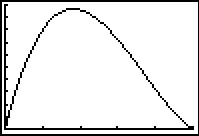
\includegraphics[width=2in]{./PolynomialsGraphics/Modeling01.jpg} \hspace{0.75in} & 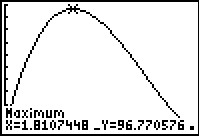
\includegraphics[width=2in]{./PolynomialsGraphics/Modeling02.jpg}

\end{tabular}
\end{center}
\vspace{-.55in} \qed
\end{enumerate}
\label{openbox}
\end{ex}


In order to solve Example \ref{openbox}, we made good use of the graph of the polynomial $y=V(x)$, so we ought to turn our attention to graphs of polynomials in general.  Below are the graphs of $y=x^2$, $y=x^4$ and $y=x^6$, side-by-side.  We have omitted the axes to allow you to see that as the exponent increases, the `bottom' becomes `flatter' and the `sides' become `steeper.'  If you take the the time to graph these functions by hand,\footnote{Make sure you choose some $x$-values between $-1$ and $1$.} you will see why. 

\smallskip

%\begin{tabular}{m{1in}m{1.5in}m{1.5in}m{1.5in}}

%&
\begin{center}
\begin{tabular}{ccc}

\begin{mfpic}[10][5]{-3.5}{3.5}{-1}{10}
\arrow \reverse \arrow \function{-3.1623,3.1623,0.1}{x**2}
\tcaption{$y=x^2$}
\end{mfpic}

\hspace{1in} &

\begin{mfpic}[10][5]{-2}{2}{-1}{10}
\arrow \reverse \arrow \function{-1.7783,1.7783,0.1}{x**4}
\tcaption{$y=x^4$}
\end{mfpic}

\hspace{1in} &

\begin{mfpic}[10][5]{-2}{2}{-1}{10}
\arrow \reverse \arrow \function{-1.4678,1.4678,0.1}{x**6}
\tcaption{$y=x^6$}
\end{mfpic}

\end{tabular}
\end{center}

All of these functions are even, (Do you remember how to show this?) and it is exactly because the exponent is even.\footnote{Herein lies one of the possible origins of the term `even' when applied to functions.} This symmetry is important, but we want to explore a different yet equally important feature of these functions which we can be seen graphically -- their \index{polynomial function ! end behavior}\index{end behavior ! of a function graph}\textbf{end behavior}.  

\smallskip

The end behavior of a function is a way to describe what is happening to the function values (the $y$-values) as the $x$-values approach the `ends' of the $x$-axis.\footnote{Of course, there are no ends to the $x$-axis.} That is, what happens to $y$ as $x$ becomes small without bound\footnote{We think of $x$ as becoming a very large (in the sense of its absolute value) \textit{negative} number far to the left of zero.} (written $x \rightarrow -\infty$) and, on the flip side, as $x$ becomes large without bound\footnote{We think of $x$ as moving far to the right of zero and becoming a very large \textit{positive} number.} (written $x \rightarrow \infty$).  

\smallskip

For example, given $f(x) = x^2$, as $x \rightarrow -\infty$, we imagine substituting $x=-100$, $x=-1000$, etc., into $f$ to get $f(-100)=10000$, $f(-1000)=1000000$, and so on. Thus  the function values are becoming larger and larger positive numbers (without bound).  To describe this behavior, we write: as $x \rightarrow -\infty$, $f(x) \rightarrow \infty$.  If we study the behavior of $f$ as $x \rightarrow \infty$, we see that in this case, too, $f(x) \rightarrow \infty$. (We told you that the symmetry was important!) The same can be said for any function of the form $f(x) = x^n$ where $n$ is an even natural number.   If we generalize just a bit to include vertical scalings and reflections across the $x$-axis,\footnote{See Theorems \ref{reflections} and \ref{vscalings} in Section \ref{Transformations}.} we have


\smallskip

\colorbox{ResultColor}{\bbm

\smallskip

\centerline{ \textbf{End Behavior of functions $f(x) = ax^{n}$, $n$ even.}}

\smallskip

Suppose $f(x) = a x^{n}$ where $a \neq 0$ is a real number and $n$ is an even natural number.  The end behavior of the graph of $y=f(x)$ matches one of the following: \index{end behavior ! of $f(x) = ax^{n}, n$ even}

\begin{itemize}

\item  for $a > 0$, as $x \rightarrow -\infty$, $f(x) \rightarrow \infty$ and as $x \rightarrow \infty$, $f(x) \rightarrow \infty$

\item  for $a < 0$, as $x \rightarrow -\infty$, $f(x) \rightarrow -\infty$ and as $x \rightarrow \infty$, $f(x) \rightarrow -\infty$

\end{itemize}

Graphically:

\begin{tabular}{m{1.5in}m{1.5in}m{1.5in}}

&

\begin{mfpic}[5]{-5}{5}{-1}{5}
\arrow \reverse \function{-5,-3, 0.1}{(x**2)/5}
\dotted \function{-3,3, 0.1}{(x**2)/5}
\arrow \function{3,5, 0.1}{(x**2)/5}
\tcaption{$a>0$}
\end{mfpic}

&

\begin{mfpic}[5]{-5}{5}{-5}{1}
\arrow \reverse \function{-5,-3, 0.1}{(0-(x**2))/5} 
\dotted \function{-3,3, 0.1}{-(x**2)/5}
\arrow \function{3,5, 0.1}{(0-(x**2))/5} 
\tcaption{$a<0$}
\end{mfpic} 

\end{tabular}

\vspace{-.2in}

\ebm}

\smallskip

We now turn our attention to functions of the form $f(x) = x^{n}$ where $n \geq 3$ is an odd natural number. (We ignore the case when $n=1$, since the graph of $f(x)=x$ is a line and doesn't fit the general pattern of higher-degree odd polynomials.) Below we have graphed $y=x^3$, $y=x^5$, and $y=x^7$.    The `flattening' and `steepening' that we saw with the even powers presents itself here as well, and, it should come as no surprise that all of these functions are odd.\footnote{And are, perhaps, the inspiration for the moniker `odd function'.}  The end behavior of these functions is all the same, with $f(x) \rightarrow -\infty$ as $x \rightarrow -\infty$ and $f(x) \rightarrow \infty$ as $x \rightarrow \infty$.


%\begin{tabular}{m{1in}m{1.5in}m{1.5in}m{1.5in}}


%&
\begin{center}

\begin{tabular}{ccc}

\begin{mfpic}[10][5]{-2}{2}{-5}{5}
\arrow \reverse \arrow \function{-1.700,1.700,0.1}{x**3}
\tcaption{$y=x^3$}
\end{mfpic}

\hspace{1in} &

\begin{mfpic}[10][5]{-2}{2}{-5}{5}
\arrow \reverse \arrow \function{-1.3800,1.3800,0.1}{x**5}
\tcaption{$y=x^5$}
\end{mfpic}

\hspace{1in} &

\begin{mfpic}[10][5]{-2}{2}{-5}{5}
\arrow \reverse \arrow \function{-1.2585,1.2585,0.1}{x**7}
\tcaption{$y=x^7$}
\end{mfpic}

\end{tabular}
\end{center}

As with the even degreed functions we studied earlier, we can generalize their end behavior.

\smallskip

\colorbox{ResultColor}{\bbm

\smallskip

\centerline{ \textbf{End Behavior of functions $f(x) = ax^{n}$, $n$ odd.}}

\smallskip

Suppose $f(x) = a x^{n}$ where $a \neq 0$ is a real number and $n \geq 3$ is an odd natural number.  The end behavior of the graph of $y=f(x)$ matches one of the following: \index{end behavior ! of $f(x) = ax^{n}, n$ odd}

\begin{itemize}

\item  for $a > 0$, as $x \rightarrow -\infty$, $f(x) \rightarrow -\infty$ and as $x \rightarrow \infty$, $f(x) \rightarrow \infty$

\item  for $a < 0$, as $x \rightarrow -\infty$, $f(x) \rightarrow \infty$ and as $x \rightarrow \infty$, $f(x) \rightarrow -\infty$

\end{itemize}

Graphically:

\medskip

\begin{tabular}{m{1.5in}m{1.5in}m{1.5in}}

&

\begin{mfpic}[5]{-5}{5}{-1}{5}
\arrow \reverse \function{-5,-3, 0.1}{0 - (x**2)/5}
\dotted \function{-3,0, 0.1}{-(x**2)/5}
\dotted \function{0,3, 0.1}{(x**2)/5}
\arrow \function{3,5, 0.1}{(x**2)/5}
\tcaption{$a>0$}
\end{mfpic}

&

\begin{mfpic}[5]{-5}{5}{-1}{5}
\arrow \reverse \function{-5,-3, 0.1}{(x**2)/5}
\dotted \function{-3,0, 0.1}{(x**2)/5}
\dotted \function{0,3, 0.1}{-(x**2)/5}
\arrow \function{3,5, 0.1}{0 - (x**2)/5}
\tcaption{$a<0$}
\end{mfpic}

\end{tabular}

\vspace{-.2in}

\ebm}

\smallskip

Despite having different end behavior, all functions of the form $f(x) = ax^{n}$ for natural numbers $n$ share two properties which help distinguish them from other animals in the algebra zoo:  they  are \index{continuous}\index{function ! continuous}\textbf{continuous} and \index{smooth}\index{function ! smooth}\textbf{smooth}.  While these concepts are formally defined using Calculus,\footnote{In fact, if you take Calculus, you'll find that smooth functions are automatically continuous, so that saying `polynomials are continuous and smooth' is redundant.} informally, graphs of continuous functions have no `breaks' or `holes' in them, and the graphs of smooth functions have no `sharp turns'.  It turns out that these traits are preserved when functions are added together, so general polynomial functions inherit these qualities.  Below we find the graph of a function which is neither smooth nor continuous, and to its right we have a graph of a polynomial, for comparison.  The function whose graph appears on the left fails to be continuous where it has a `break' or `hole' in the graph;  everywhere else, the function is continuous.  The function is continuous at the `corner' and the `cusp', but we consider these `sharp turns', so these are places where the function fails to be smooth.  Apart from these four places, the function is smooth and continuous.  Polynomial functions are smooth and continuous everywhere, as exhibited in the graph on the right.

\phantomsection
\label{cusppicture} 

\medskip

\begin{center}

%\begin{tabular}{m{0.25in}m{2.5in}m{2.5in}}

%& 

\begin{tabular}{cc}

\begin{mfpic}[15]{-5}{5}{-2}{5}
\arrow \polyline{(-3,2),(-5,4)}
\arrow \function{-3,-1.5,0.1}{1-(2/(x+1))}
\dashed \polyline{(-1,0),(-1,5)}
\arrow \parafcn{-1,1.75,0.1}{(t**3,(t**2)+1)} 
\point[3pt]{(-1,2)}
\gclear \circle{(3.375,3.25),0.1}
\circle{(3.375,3.25),0.1}
\tlabel[cc](-3,1.5){\tiny `corner'}
\tlabel[cc](-1,-0.5){\tiny`break'}
\tlabel[cc](0,0.5){\tiny`cusp'}
\tlabel[cc](3.375,2.5){\tiny`hole'}
\tcaption{\tiny  Pathologies not found on graphs of polynomials}
\end{mfpic}

\hspace{0.75in} &

\begin{mfpic}[15][7.5]{-5}{5}{-10}{10}
\arrow \reverse \arrow \function{-3,3.5,0.1}{0.5*x*(x+2)*(x-3)}
\tcaption{\tiny  The graph of a polynomial}
\end{mfpic}

\end{tabular}

\end{center}

The notion of smoothness is what tells us graphically that, for example, $f(x) = |x|$, whose graph is the characteristic `$\vee$' shape, cannot be a polynomial.  The notion of continuity is what allowed us to construct the sign diagram for quadratic inequalities as we did in Section \ref{Inequalities}.  This last result is formalized in the following theorem.
  
\smallskip

\colorbox{ResultColor}{\bbm

\begin{thm} \textbf{The Intermediate Value Theorem (Zero Version):}  Suppose $f$ is a continuous function on an interval containing $x=a$ and $x=b$ with $a<b$. If $f(a)$ and $f(b)$ have different signs, then $f$ has at least one zero between $x = a$ and $x = b$;  that is, for at least one real number $c$ such that $a < c < b$, we have $f(c) = 0$. \index{Intermediate Value Theorem ! polynomial zero version}


\label{IVT}
\end{thm}

\ebm}

\smallskip

The Intermediate Value Theorem is extremely profound;  it gets to the heart of what it means to be a real number, and is one of the most often used and under appreciated theorems in Mathematics.  With that being said, most students see the result as common sense since it says, geometrically, that the graph of a polynomial function cannot be above the $x$-axis at one point and below the $x$-axis at another point without crossing the $x$-axis somewhere in between.  The following example uses the Intermediate Value Theorem to establish a fact that that most students take for granted.  Many students, and sadly some instructors, will find it silly.

\begin{ex}  Use the Intermediate Value Theorem to establish that $\sqrt{2}$ is a real number.

\smallskip

{\bf Solution.}  Consider the polynomial function $f(x) = x^2 - 2$.  Then $f(1) = -1$ and $f(3) = 7$.  Since $f(1)$ and $f(3)$ have different signs, the Intermediate Value Theorem guarantees us a real number $c$ between $1$ and $3$ with $f(c) = 0$.  If $c^2 - 2 = 0$ then $c = \pm \sqrt{2}$.  Since $c$ is between $1$ and $3$, $c$ is positive, so $c = \sqrt{2}$. \qed

\end{ex}

Our primary use of the Intermediate Value Theorem is in the construction of sign diagrams, as in Section \ref{Inequalities}, since it guarantees us that polynomial functions are always positive $(+)$ or always negative $(-)$ on intervals which do not contain any of its zeros.  The general algorithm for polynomials is given below.

\smallskip
\colorbox{ResultColor}{\bbm

\centerline{\textbf{Steps for Constructing a Sign Diagram for a Polynomial Function}}

\smallskip

\hspace{.17in} Suppose $f$ is a polynomial function. \index{sign diagram ! polynomial function}

\begin{enumerate}

\item  Find the zeros of $f$ and place them on the number line with the number $0$ above them.

\item  Choose a real number, called a \textbf{test value}, in each of the intervals determined in step 1. 

\item  Determine the sign of $f(x)$ for each test value in step 2, and write that sign above the corresponding interval.

\end{enumerate}

\ebm}
\smallskip 

\begin{ex}  Construct a sign diagram for $f(x) = x^3 (x-3)^2 (x+2) \left(x^2+1\right)$.   Use it to give a rough sketch of the graph of  $y=f(x)$.  \label{polygraphex}

\smallskip

{\bf Solution.}  First, we find the zeros of $f$ by solving $x^3 (x-3)^2 (x+2)\left(x^2+1\right)=0$.   We get $x=0$, $x=3$ and $x=-2$. (The equation $x^2+1=0$ produces no real solutions.)  These three points divide the real number line into four intervals:  $(-\infty, -2)$, $(-2,0)$, $(0,3)$ and $(3,\infty)$.  We select the test values $x=-3$, $x=-1$, $x=1$ and $x=4$. We find $f(-3)$ is $(+)$, $f(-1)$ is $(-)$ and $f(1)$ is $(+)$ as is $f(4)$.  Wherever $f$ is $(+)$, its graph is above the $x$-axis;  wherever $f$ is $(-)$, its graph is below the $x$-axis.  The $x$-intercepts of the graph of $f$ are $(-2,0)$, $(0,0)$ and $(3,0)$.  Knowing $f$ is smooth and continuous allows us to sketch its graph.

\begin{tabular}{m{0.5in}m{2.5in}m{2.5in}}

&

\begin{mfpic}[10]{-8}{8}{-2}{30}
\arrow \reverse \arrow \polyline{(-8,0),(8,0)}
\xmarks{-3,0,3}
\arrow \polyline{(-5,-1.5),(-5,-0.5)}
\arrow \polyline{(-1.5,-1.5),(-1.5,-0.5)}
\arrow \polyline{(1.5,-1.5),(1.5,-0.5)}
\arrow \polyline{(5,-1.5),(5,-0.5)}
\tlpointsep{4pt}
\axislabels {x}{{$-2$} -3, {$0$} 0, {$3$} 3 }
\tlabel[cc](-5,1){$(+)$}
\tlabel[cc](-5,-2.25){$-3$}
\tlabel[cc](-3,1){$0$}
\tlabel[cc](-1.5,1){$(-)$}
\tlabel[cc](-1.75,-2.25){$-1$}
\tlabel[cc](0,1){$0$}
\tlabel[cc](1.5,1){$(+)$}
\tlabel[cc](1.5,-2.25){$1$}
\tlabel[cc](3,1){$0$}
\tlabel[cc](5,1){$(+)$}
\tlabel[cc](5,-2.25){$4$}
\end{mfpic} 

&

\begin{mfpic}[15]{-5}{5}{-2}{3}
\arrow \reverse \arrow \function{-2.2,3.5, 0.1}{0.05*((x)**3)*(x+2)*((x-3)**2)} 
\axes
\tlabel[cc](5,-0.5){\scriptsize $x$}
\tlabel[cc](0.5,3){\scriptsize $y$}
\point[3pt]{(-2,0), (0,0), (3,0)}
\xmarks{-4,-3,-2,-1,1,2,3,4}
\tcaption{ \scriptsize A sketch of $y=f(x)$}
\end{mfpic} 

\end{tabular}

\vspace{-.35in}

\qed

\end{ex}

A couple of notes about the Example \ref{polygraphex} are in order.  First, note that we purposefully did not label the $y$-axis in the sketch of the graph of $y=f(x)$.  This is because the sign diagram gives us the zeros and the relative position of the graph - it doesn't give us any information as to how high or low the graph strays from the $x$-axis.  Furthermore, as we have mentioned earlier in the text, without Calculus, the values of the relative maximum and minimum can only be found approximately using a calculator.  If we took the time to find the leading term of $f$, we would find it to be $x^8$.  Looking at the end behavior of $f$, we notice that it matches the end behavior of $y=x^8$.  This is no accident, as we find out in the next theorem.

\medskip

\colorbox{ResultColor}{\bbm

\begin{thm} \label{EBPolynomials}\index{end behavior ! polynomial}\textbf{End Behavior for Polynomial Functions:} The end behavior of a polynomial $f(x) = a_{n} x^{n} + a_{n-\mbox{\tiny$1$}} x^{n-\mbox{\tiny$1$}} + \ldots + a_{\mbox{\tiny $2$}} x^{\mbox{\tiny $2$}} + a_{\mbox{\tiny $1$}} x + a_{\mbox{\tiny $0$}}$ with $a_{n} \neq 0$ matches the end behavior of $y = a_{n} x^{n}$.  
\end{thm}

\ebm}

\medskip

To see why Theorem \ref{EBPolynomials} is true, let's first look at a specific example.  Consider $f(x) = 4x^3 - x + 5$.  If we wish to examine end behavior, we look to see the behavior of $f$ as $x \rightarrow \pm \infty$.  Since we're concerned with $x$'s far down the $x$-axis, we are far away from $x=0$ so can rewrite $f(x)$ for these values of $x$ as \[ f(x) = 4x^3 \left( 1 - \dfrac{1}{4x^2} + \dfrac{5}{4x^3}\right)\]

As $x$ becomes unbounded (in either direction), the terms $\frac{1}{4x^2}$ and $\frac{5}{4x^3}$ become closer and closer to $0$, as the table below indicates.


\[ \begin{array}{|r||r|r|}  

\hline 

 x & \frac{1}{4x^2} & \frac{5}{4x^3} \vphantom{\dfrac{a}{a}} \\ [2pt] \hline
-1000  & 0.00000025 & -0.00000000125 \\  \hline
-100  & 0.000025 & -0.00000125 \\  \hline
-10 & 0.0025 & -0.00125 \\  \hline
10  & 0.0025 & 0.00125 \\  \hline
100 & 0.000025 & 0.00000125 \\  \hline
1000 & 0.00000025 & 0.00000000125 \\  \hline
\end{array} \]

\smallskip

In other words, as $x \rightarrow \pm \infty$, $f(x) \approx 4x^3\left( 1 - 0 +0\right) = 4x^3$, which is the leading term of $f$.  The formal proof of Theorem \ref{EBPolynomials} works in much the same way.  Factoring out the leading term leaves

\[ f(x) = a_{n} x^{n} \left( 1 + \dfrac{a_{n-\mbox{\tiny$1$}}}{a_{n} x}+ \ldots + \dfrac{a_{\mbox{\tiny$2$}}}{a_{n} x^{n-2}} + \dfrac{a_{\mbox{\tiny$1$}}}{a_{n} x^{n-1}}+\dfrac{a_{\mbox{\tiny$0$}}}{a_{n} x^{n}}\right)\]

As $x \rightarrow \pm \infty$, any term with an $x$ in the denominator becomes closer and closer to $0$, and we have $f(x) \approx a_{n} x^{n}$.  Geometrically, Theorem \ref{EBPolynomials} says that if we graph $y=f(x)$ using a graphing calculator, and continue to `zoom out', the graph of it and its leading term become indistinguishable.  Below are the graphs of $y=4x^3-x+5$ (the thicker line) and $y=4x^3$ (the thinner line) in two different windows.

\begin{center}

\begin{tabular}{cc}

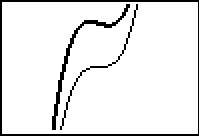
\includegraphics[width=2in]{./PolynomialsGraphics/EB01.jpg} \hspace{.25in} & 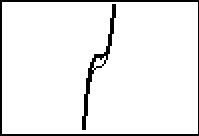
\includegraphics[width=2in]{./PolynomialsGraphics/EB02.jpg} \\

A view `close' to the origin. \hspace{.25in} & A `zoomed out' view. \\

\end{tabular}

\end{center}

Let's return to the function in Example \ref{polygraphex}, $f(x) = x^3 (x-3)^2 (x+2)\left(x^2+1\right)$, whose sign diagram and graph are reproduced below for reference.  Theorem \ref{EBPolynomials} tells us that the end behavior is the same as that of its leading term $x^{8}$.  This tells us that the graph of $y=f(x)$ starts and ends above the $x$-axis.  In other words, $f(x)$ is $(+)$ as $x \rightarrow \pm \infty$, and as a result, we no longer need to evaluate $f$ at the test values $x=-3$ and $x=4$.  Is there a way to eliminate the need to evaluate $f$ at the other test values?  What we would really need to know is how the function behaves near its zeros - does it cross through the $x$-axis at these points, as it does at $x=-2$ and $x=0$, or does it simply touch and rebound like it does at $x=3$.  From the sign diagram, the graph of $f$ will cross the $x$-axis whenever the signs on either side of the zero switch (like they do at $x=-2$ and $x=0$);  it will touch when the signs are the same on either side of the zero (as is the case with $x=3$). What we need to determine is the reason behind whether or not the sign change occurs.

\begin{tabular}{m{0.5in}m{2.5in}m{2.5in}}

&

\begin{mfpic}[10]{-8}{8}{-2}{2}
\arrow \reverse \arrow \polyline{(-8,0),(8,0)}
\xmarks{-3,0,3}
\arrow \polyline{(-5,-1.5),(-5,-0.5)}
\arrow \polyline{(-1.5,-1.5),(-1.5,-0.5)}
\arrow \polyline{(1.5,-1.5),(1.5,-0.5)}
\arrow \polyline{(5,-1.5),(5,-0.5)}
\tlpointsep{4pt}
\axislabels {x}{{$-2$} -3, {$0$} 0, {$3$} 3 }
\tlabel[cc](-5,1){$(+)$}
\tlabel[cc](-5,-2.25){$-3$}
\tlabel[cc](-3,1){$0$}
\tlabel[cc](-1.5,1){$(-)$}
\tlabel[cc](-1.75,-2.25){$-1$}
\tlabel[cc](0,1){$0$}
\tlabel[cc](1.5,1){$(+)$}
\tlabel[cc](1.5,-2.25){$1$}
\tlabel[cc](3,1){$0$}
\tlabel[cc](5,1){$(+)$}
\tlabel[cc](5,-2.25){$4$}
\end{mfpic} 

&

\begin{mfpic}[15]{-5}{5}{-2}{3}
\arrow \reverse \arrow \function{-2.2,3.5, 0.1}{0.05*((x)**3)*(x+2)*((x-3)**2)} 
\axes
\tlabel[cc](5,-0.5){\scriptsize $x$}
\tlabel[cc](0.5,3){\scriptsize $y$}
\point[3pt]{(-2,0), (0,0), (3,0)}
\xmarks{-4,-3,-2,-1,1,2,3,4}
\tcaption{ \scriptsize A sketch of $y=f(x)$}
\end{mfpic} 

\end{tabular}

Fortunately, $f$ was given to us in factored form:  $f(x) = x^3 (x-3)^2 (x+2)$.  When we attempt to determine the sign of $f(-4)$, we are attempting to find the sign of the number $(-4)^3 (-7)^2 (-2)$, which works out to be $(-)(+)(-)$ which is $(+)$.  If we move to the other side of $x=-2$, and find the sign of $f(-1)$, we are determining the sign of  $(-1)^3 (-4)^2 (+1)$, which is $(-)(+)(+)$ which gives us the $(-)$.  Notice that signs of the first two factors in both expressions are the same in $f(-4)$ and $f(-1)$.  The only factor which switches sign is the third factor, $(x+2)$, precisely the factor which gave us the zero $x=-2$.  If we move to the other side of $0$ and look closely at $f(1)$, we get the sign pattern $(+1)^3(-2)^2(+3)$ or $(+)(+)(+)$ and we note that, once again, going from $f(-1)$ to $f(1)$, the only factor which changed sign was the first factor, $x^3$, which corresponds to the zero $x=0$.  Finally, to find $f(4)$, we substitute to get $(+4)^3(+2)^2(+5)$ which is $(+)(+)(+)$ or $(+)$.  The sign didn't change for the middle factor $(x-3)^2$.  Even though this is the factor which corresponds to the zero $x=3$, the fact that the quantity is \textit{squared} kept the sign of the middle factor the same on either side of $3$.  If we look back at the exponents on the factors $(x+2)$ and $x^3$, we see that they are both odd, so as we substitute values to the left and right of the corresponding zeros, the signs of the corresponding factors change which results in the sign of the function value changing.  This is the key to the behavior of the function near the zeros.  We need a definition and then a theorem.

\smallskip

\colorbox{ResultColor}{\bbm

\begin{defn} \label{multiplicity} Suppose $f$ is a polynomial function and $m$ is a natural number. If $(x-c)^{m}$ is a factor of $f(x)$ but $(x-c)^{m+1}$ is not, then we say $x=c$ is a zero of \index{polynomial function ! zero ! multiplicity}\index{multiplicity ! of a zero}\index{zero ! multiplicity of}\textbf{multiplicity} $m$.

\end{defn}

\ebm}

\smallskip

Hence,  rewriting  $f(x) = x^3 (x-3)^2 (x+2)$ as $f(x) = (x-0)^3 (x-3)^2 (x-(-2))^{1}$, we see that $x=0$ is a zero of multiplicity $3$, $x=3$ is a zero of multiplicity $2$ and $x=-2$ is a zero of multiplicity $1$.

\smallskip

\colorbox{ResultColor}{\bbm

\begin{thm} \label{roleofmultiplicity} \textbf{The Role of Multiplicity:}  Suppose $f$ is a polynomial function  and $x=c$ is a zero of multiplicity $m$.  \index{multiplicity ! effect on the graph of a polynomial}

\begin{itemize}

\item  If $m$ is even, the graph of $y=f(x)$ touches and rebounds from the $x$-axis at $(c,0)$.

\item  If $m$ is odd, the graph of $y=f(x)$ crosses through the $x$-axis at $(c,0)$.

\end{itemize}

\end{thm}

\ebm}

\medskip

Our last example shows how end behavior and multiplicity allow us to sketch a decent graph without appealing to a sign diagram.

\begin{ex}  Sketch the graph of $f(x) = -3(2x-1)(x+1)^2$ using end behavior and the multiplicity of its zeros.

\bigskip

{ \bf Solution.}  The end behavior of the graph of $f$ will match that of its leading term.  To find the leading term, we multiply by the leading terms of each factor to get $(-3)(2x)(x)^2 = -6x^3$.  This tells us that the graph will start above the $x$-axis, in Quadrant II, and finish below the $x$-axis, in Quadrant IV.  Next, we find the zeros of $f$.  Fortunately for us, $f$ is factored.\footnote{Obtaining the factored form of a polynomial is the main focus of the next few sections.}  Setting each factor equal to zero gives is $x = \frac{1}{2}$ and $x=-1$ as zeros. To find the multiplicity of $x=\frac{1}{2}$ we note that it corresponds to the factor $(2x-1)$.  This isn't strictly in the form required in Definition \ref{multiplicity}.  If we factor out the $2$, however, we get $(2x-1) = 2\left(x-\frac{1}{2}\right)$, and we see that the multiplicity of $x = \frac{1}{2}$ is $1$.  Since $1$ is an odd number, we know from Theorem \ref{roleofmultiplicity} that the graph of $f$ will cross through the $x$-axis at $\left(\frac{1}{2},0\right)$.   Since the zero $x=-1$ corresponds to the factor $(x+1)^2 = (x-(-1))^2$, we find its multiplicity to be $2$ which is an even number.  As such, the graph of $f$ will touch and rebound from the $x$-axis at $(-1,0)$.  Though we're not asked to, we can find the $y$-intercept by finding $f(0) = -3(2(0)-1)(0+1)^2 = 3$.  Thus  $(0,3)$ is an additional point on the graph.  Putting this together gives us the graph below.

\begin{center}

\begin{mfpic}[20][10]{-3}{3}{-5}{5}
\arrow \reverse \arrow \function{-1.75,0.75,0.1}{0-1.5*(2*x-1)*((x+1)**2)}
\axes
\tlabel[cc](3,-0.5){\scriptsize $x$}
\tlabel[cc](0.5,5){\scriptsize $y$}
\point[3pt]{(0.5,0), (-1,0), (0,1.5) }
\xmarks{-2,-1,0,1,2}
\ymarks{0.5, 1.0, 1.5, 2}
\end{mfpic}

\end{center} 

\vspace{-.25in}

\qed

\end{ex}

\newpage

\subsection{Exercises}

In Exercises \ref{polyfactsfirst} - \ref{polyfactslast}, find the degree, the leading term, the leading coefficient, the constant term and the end behavior of the given polynomial.

\begin{multicols}{2}
\begin{enumerate}

\item  $f(x) = 4-x-3x^2$ \label{polyfactsfirst}
\item  $g(x) = 3x^5 - 2x^2 + x + 1$

\setcounter{HW}{\value{enumi}}
\end{enumerate}
\end{multicols}

\begin{multicols}{2}
\begin{enumerate}
\setcounter{enumi}{\value{HW}}

\item $q(r) = 1 - 16r^{4}$
\item $Z(b) = 42b - b^{3}$

\setcounter{HW}{\value{enumi}}
\end{enumerate}
\end{multicols}

\begin{multicols}{2}
\begin{enumerate}
\setcounter{enumi}{\value{HW}}

\item $f(x) = \sqrt{3}x^{17} + 22.5x^{10} - \pi x^{7} + \frac{1}{3}$
\item $s(t) = -4.9t^{2} + v_{\mbox{\tiny $0$}}t + s_{\mbox{\tiny $0$}}$

\setcounter{HW}{\value{enumi}}
\end{enumerate}
\end{multicols}

\begin{multicols}{2}
\begin{enumerate}
\setcounter{enumi}{\value{HW}}

\item $P(x) = (x - 1)(x - 2)(x - 3)(x - 4)$
\item $p(t) = -t^2(3 - 5t)(t^{2} + t + 4)$

\setcounter{HW}{\value{enumi}}
\end{enumerate}
\end{multicols}

\begin{multicols}{2}
\begin{enumerate}
\setcounter{enumi}{\value{HW}}

\item $f(x) = -2x^3(x+1)(x+2)^2$
\item $G(t) = 4(t-2)^2\left(t+\frac{1}{2}\right)$ \label{polyfactslast}

\setcounter{HW}{\value{enumi}}
\end{enumerate}
\end{multicols}

\phantomsection
\label{polygraphexercise}

In Exercises \ref{zeromultgraphfirst} - \ref{zeromultgraphlast}, find the real zeros of the given polynomial and their corresponding multiplicities.  Use this information along with a sign chart to provide a rough sketch of the graph of the polynomial.  Compare your answer with the result from a graphing utility.

\begin{multicols}{2}
\begin{enumerate}
\setcounter{enumi}{\value{HW}}

\item $a(x) = x(x + 2)^{2}$ \label{zeromultgraphfirst}
\item $g(x) = x(x + 2)^{3}$

\setcounter{HW}{\value{enumi}}
\end{enumerate}
\end{multicols}


\begin{multicols}{2}
\begin{enumerate}
\setcounter{enumi}{\value{HW}}

\item $f(x) = -2(x-2)^2(x+1)$
\item $g(x) = (2x+1)^2(x-3)$

\setcounter{HW}{\value{enumi}}
\end{enumerate}
\end{multicols}


\begin{multicols}{2}
\begin{enumerate}
\setcounter{enumi}{\value{HW}}

\item $F(x) = x^{3}(x + 2)^{2}$
\item $P(x) = (x - 1)(x - 2)(x - 3)(x - 4)$

\setcounter{HW}{\value{enumi}}
\end{enumerate}
\end{multicols}


\begin{multicols}{2}
\begin{enumerate}
\setcounter{enumi}{\value{HW}}

\item $Q(x) = (x + 5)^{2}(x - 3)^{4}$
\item $h(x) = x^2(x-2)^2(x+2)^2$

\setcounter{HW}{\value{enumi}}
\end{enumerate}
\end{multicols}


\begin{multicols}{2}
\begin{enumerate}
\setcounter{enumi}{\value{HW}}

\item $H(t) = (3-t)(t^2+1)$
\item $Z(b) = b(42 - b^{2})$ \label{zeromultgraphlast}

\setcounter{HW}{\value{enumi}}
\end{enumerate}
\end{multicols}

In Exercises \ref{polytransfirst} - \ref{polytranslast}, given the pair of functions $f$ and $g$, sketch the graph of $y=g(x)$ by starting with the graph of $y = f(x)$ and using transformations.  Track at least three points of your choice through the transformations. State the domain and range of $g$.

\begin{multicols}{2}
\begin{enumerate}
\setcounter{enumi}{\value{HW}}

\item $f(x) = x^3$,  $g(x) = (x + 2)^{3} + 1$ \label{polytransfirst}
\item $f(x) = x^4$, $g(x) = (x + 2)^{4} + 1$

\setcounter{HW}{\value{enumi}}
\end{enumerate}
\end{multicols}

\begin{multicols}{2}
\begin{enumerate}
\setcounter{enumi}{\value{HW}}

\item $f(x) = x^4$, $g(x) = 2 - 3(x - 1)^{4}$
\item $f(x) = x^5$, $g(x) = -x^{5} - 3$

\setcounter{HW}{\value{enumi}}
\end{enumerate}
\end{multicols}

\begin{multicols}{2}
\begin{enumerate}
\setcounter{enumi}{\value{HW}}

\item $f(x) = x^5$, $g(x) = (x+1)^5+10$
\item $f(x) = x^6$, $g(x) = 8-x^6$ \label{polytranslast}

\setcounter{HW}{\value{enumi}}
\end{enumerate}
\end{multicols}

\begin{enumerate}
\setcounter{enumi}{\value{HW}}

\item Use the Intermediate Value Theorem to prove that $f(x) = x^{3} - 9x + 5$ has a real zero in each of the following intervals: $[-4, -3], [0, 1]$ and $[2, 3]$.

\item  Rework Example \ref{boxnotopex} assuming the box is to be made from an 8.5 inch by 11 inch sheet of paper. Using scissors and tape, construct the box.  Are you surprised?\footnote{Consider decorating the box and presenting it to your instructor. If done well enough, maybe your instructor will issue you some bonus points.  Or maybe not.}

\setcounter{HW}{\value{enumi}}
\end{enumerate}

\phantomsection
\label{LCDmaxprofit} 

In Exercises \ref{lcdmaxprofitexerfirst} - \ref{lcdmaxprofitexerlast}, suppose the revenue $R$, in \textit{thousands} of dollars, from producing and selling $x$ \textit{hundred} LCD TVs is given by $R(x) = -5x^3+35x^2+155x$ for $0 \leq x \leq 10.07$.

\begin{enumerate}
\setcounter{enumi}{\value{HW}}

\item  Use a graphing utility to graph $y = R(x)$ and determine the number of TVs which should be sold to maximize revenue.  What is the maximum revenue? \label{lcdmaxprofitexerfirst}

\item Assume that the cost, in \textit{thousands} of dollars, to produce $x$ \textit{hundred} LCD TVs is given by $C(x) = 200x + 25$ for $x \geq 0$. Find and simplify an expression for the profit function $P(x)$.  (Remember: Profit = Revenue - Cost.)

\item  Use a graphing utility to graph $y = P(x)$ and determine the number of TVs which should be sold to maximize profit.  What is the maximum  profit? \label{lcdmaxprofitexerlast}

\item \label{newportaboycost} While developing their newest game, Sasquatch Attack!, the makers of the PortaBoy (from Example \ref{PortaBoyCost}) revised their cost function and now use $C(x) = .03x^{3} - 4.5x^{2} + 225x + 250$, for $x \geq 0$. As before, $C(x)$ is the cost to make $x$ PortaBoy Game Systems.  Market research indicates that the demand function $p(x) = -1.5x + 250$ remains unchanged.  Use a graphing utility to find the production level $x$ that maximizes the \textit{profit} made by producing and selling $x$ PortaBoy game systems.

\setcounter{HW}{\value{enumi}}
\end{enumerate}

\begin{enumerate}
\setcounter{enumi}{\value{HW}}

\item According to US Postal regulations, a rectangular shipping box must satisfy the inequality ``Length + Girth $\leq$ 130 inches'' for Parcel Post and ``Length + Girth $\leq$ 108 inches'' for other services. Let's assume we have a closed rectangular box with a square face of side length $x$ as drawn below.  The length is the longest side and is clearly labeled.  The girth is the distance around the box in the other two dimensions so in our case it is the sum of the four sides of the square, $4x$.  

\begin{enumerate}

\item \label{girthbox1} Assuming that we'll be mailing a box via Parcel Post where Length + Girth $=$ 130 inches, express the length of the box in terms of $x$ and then express the volume $V$ of the box in terms of $x$.

\item \label{girthbox2} Find the dimensions of the box of maximum volume that can be shipped via Parcel Post.

\item Repeat parts \ref{girthbox1} and \ref{girthbox2} if the box is shipped using ``other services''.

\end{enumerate}

\begin{center}

\begin{mfpic}[8]{-6}{12}{-1}{17}
\polyline{(0,0),(-4,3)}
\polyline{(-4,3), (-4,8)}
\polyline{(-4,8),(0,5)}
\polyline{(0,5),(0,0)}
\polyline{(0,0),(12,9)}
\polyline{(0,5),(12,14)}
\polyline{(-4,8),(8,17)}
\polyline{(8,17),(12,14)}
\polyline{(12,14),(12,9)}
\arrow \reverse \arrow \polyline{(0,-0.5),(12,8.5)}
\tlabel[cc](8,4){\tiny length}
\arrow \reverse \arrow \polyline{(-4, 2.5), (-0.5,-0.125)}
\tlabel[cc](-3,0.5){\tiny $x$}
\arrow \reverse \arrow \polyline{(-4.5, 3), (-4.5,8)}
\tlabel[cc](-5,5){\tiny $x$}
\end{mfpic}

\end{center}

\setcounter{HW}{\value{enumi}}
\end{enumerate}

\begin{enumerate}
\setcounter{enumi}{\value{HW}}


\item We now revisit the data set from Exercise \ref{regsunlight} in Section \ref{Regression}.  In that exercise, you were given a chart of the number of hours of daylight they get on the $21^{\mbox{st}}$ of each month in Fairbanks, Alaska based on the 2009 sunrise and sunset data found on the  \href{http://aa.usno.navy.mil/data/docs/RS_OneYear.php}{\underline{U.S. Naval Observatory}} website.  We let $x = 1$ represent January 21, 2009, $x = 2$ represent February 21, 2009, and so on.  The chart is given again for reference.

\medskip

\small

\noindent \begin{tabular}{|l|r|r|r|r|r|r|r|r|r|r|r|r|} \hline
Month  & & & & & & & & & & & & \\
Number & 1 & 2 & 3 & 4 & 5 & 6 & 7 & 8 & 9 & 10 & 11 & 12\\ 
\hline 
Hours of  & & & & & & & & & & & & \\
Daylight & 5.8 & 9.3 & 12.4 & 15.9 & 19.4 & 21.8 & 19.4 & 15.6 & 12.4 & 9.1 & 5.6 & 3.3 \\ \hline
\end{tabular}

\normalsize

\medskip

\noindent Find cubic (third degree) and quartic (fourth degree) polynomials which model this data and comment on the goodness of fit for each.  What can we say about using either model to make predictions about the year 2020?  (Hint: Think about the end behavior of polynomials.)  Use the models to see how many hours of daylight they got on your birthday and then check the website to see how accurate the models are.  Knowing that Sasquatch are largely nocturnal, what days of the year according to your models are going to allow for at least 14 hours of darkness for field research on the elusive creatures? 

\item \label{circuitexercisepoly} An electric circuit is built with a variable resistor installed.  For each of the following resistance values (measured in kilo-ohms, $k \Omega$),  the corresponding power to the load (measured in milliwatts, $mW$) is given in the table below. \footnote{The authors wish to thank Don Anthan and Ken White of Lakeland Community College for devising this problem and generating the accompanying data set.}

\noindent \begin{tabular}{|l|r|r|r|r|r|r|} \hline
Resistance: ($k \Omega$) & 1.012 & 2.199 & 3.275 & 4.676 & 6.805 & 9.975 \\ \hline
Power: ($mW$) & 1.063 & 1.496 & 1.610 & 1.613 & 1.505 & 1.314 \\ \hline
\end{tabular}

\begin{enumerate}

\item Make a scatter diagram of the data using the Resistance as the independent variable and Power as the dependent variable.

\item Use your calculator to find quadratic (2nd degree), cubic (3rd degree) and quartic (4th degree) regression models for the data and judge the reasonableness of each.

\item For each of the models found above, find the predicted maximum power that can be delivered to the load.  What is the corresponding resistance value?

\item Discuss with your classmates the limitations of these models - in particular, discuss the end behavior of each.

\end{enumerate}

\item Show that the end behavior of a linear function $f(x) = mx + b$ is as it should be according to the results we've established in the section for polynomials of odd degree.\footnote{Remember, to be a linear function, $m \neq 0$.}  (That is, show that the graph of a linear function is ``up on one side and down on the other'' just like the graph of $y = a_{n}x^{n}$ for odd numbers $n$.)

\item \index{multiplicity ! effect on the graph of a polynomial} There is one subtlety about the role of multiplicity that we need to discuss further; specifically we need to see `how' the graph crosses the $x$-axis at a zero of odd multiplicity.  In the section, we deliberately excluded the function $f(x) = x$ from the discussion of the end behavior of $f(x) = x^{n}$ for odd numbers $n$ and we said at the time that it was due to the fact that $f(x) = x$ didn't fit the pattern we were trying to establish.  You just showed in the previous exercise that the end behavior of a linear function behaves like every other polynomial of odd degree, so what doesn't $f(x) = x$ do that $g(x) = x^{3}$ does?  It's the `flattening' for values of $x$ near zero.  It is this local behavior that will distinguish between a zero of multiplicity 1 and one of higher odd multiplicity.  Look again closely at the graphs of $a(x) = x(x + 2)^{2}$ and $F(x) = x^{3}(x + 2)^{2}$ from Exercise \ref{polygraphexercise}.  Discuss with your classmates how the graphs are fundamentally different at the origin.  It might help to use a graphing calculator to zoom in on the origin to see the different crossing behavior. Also compare the behavior of $a(x) = x(x + 2)^{2}$ to that of $g(x) = x(x + 2)^{3}$ near the point $(-2, 0)$.  What do you predict will happen at the zeros of $f(x) = (x - 1)(x - 2)^2(x - 3)^{3}(x - 4)^{4}(x - 5)^{5}$?

\item Here are a few other questions for you to discuss with your classmates.  

\begin{enumerate}

\item How many local extrema could a polynomial of degree $n$ have?  How few local extrema can it have?
\item Could a polynomial have two local maxima but no local minima?  
\item If a polynomial has two local maxima and two local minima, can it be of odd degree?  Can it be of even degree?
\item Can a polynomial have local extrema without having any real zeros?
\item Why must every polynomial of odd degree have at least one real zero?
\item Can a polynomial have two distinct real zeros and no local extrema?
\item Can an $x$-intercept yield a local extrema?  Can it yield an absolute extrema?
\item If the $y$-intercept yields an absolute minimum, what can we say about the degree of the polynomial and the sign of the leading coefficient?   

\end{enumerate}

\setcounter{HW}{\value{enumi}}
\end{enumerate}
\newpage

\subsection{Answers}

\begin{multicols}{2}
\begin{enumerate}

\item $f(x) = 4-x-3x^2$ \\
Degree 2 \\
Leading term $-3x^{2}$\\
Leading coefficient $-3$\\
Constant term $4$\\
As $x \rightarrow -\infty, \; f(x) \rightarrow -\infty$\\
As $x \rightarrow \infty, \; f(x) \rightarrow -\infty$\\

\item  $g(x) = 3x^5 - 2x^2 + x + 1$ \\
Degree 5 \\
Leading term $3x^5$\\
Leading coefficient $3$\\
Constant term $1$\\
As $x \rightarrow -\infty, \; g(x) \rightarrow -\infty$\\
As $x \rightarrow \infty, \; g(x) \rightarrow \infty$\\


\setcounter{HW}{\value{enumi}}
\end{enumerate}
\end{multicols}

\begin{multicols}{2}
\begin{enumerate}
\setcounter{enumi}{\value{HW}}

\item $q(r) = 1 - 16r^{4}$\\
Degree 4 \\
Leading term $-16r^{4}$\\
Leading coefficient $-16$\\
Constant term $1$\\
As $r \rightarrow -\infty, \; q(r) \rightarrow -\infty$\\
As $r \rightarrow \infty, \; q(r) \rightarrow -\infty$\\

\item $Z(b) = 42b - b^{3}$\\
Degree 3 \\
Leading term $-b^{3}$\\
Leading coefficient $-1$\\
Constant term $0$\\
As $b \rightarrow -\infty, \; Z(b) \rightarrow \infty$\\
As $b \rightarrow \infty, \; Z(b) \rightarrow -\infty$\\

\setcounter{HW}{\value{enumi}}
\end{enumerate}
\end{multicols}

\begin{multicols}{2}
\begin{enumerate}
\setcounter{enumi}{\value{HW}}

\item $f(x) = \sqrt{3}x^{17} + 22.5x^{10} - \pi x^{7} + \frac{1}{3}$\\
Degree 17 \\
Leading term $\sqrt{3}x^{17}$\\
Leading coefficient $\sqrt{3}$\\
Constant term $\frac{1}{3}$\\
As $x \rightarrow -\infty, \; f(x) \rightarrow -\infty$\\
As $x \rightarrow \infty, \; f(x) \rightarrow \infty$\\


\item $s(t) = -4.9t^{2} + v_{\mbox{\tiny $0$}}t + s_{\mbox{\tiny $0$}}$\\
Degree 2 \\
Leading term $-4.9t^{2}$\\
Leading coefficient $-4.9$\\
Constant term $s_{\mbox{\tiny $0$}}$\\
As $t \rightarrow -\infty, \; s(t) \rightarrow -\infty$\\
As $t \rightarrow \infty, \; s(t) \rightarrow -\infty$\\


\setcounter{HW}{\value{enumi}}
\end{enumerate}
\end{multicols}

\begin{multicols}{2}
\begin{enumerate}
\setcounter{enumi}{\value{HW}}


\item $P(x) = (x - 1)(x - 2)(x - 3)(x - 4)$\\
Degree 4 \\
Leading term $x^{4}$\\
Leading coefficient $1$\\
Constant term $24$\\
As $x \rightarrow -\infty, \; P(x) \rightarrow \infty$\\
As $x \rightarrow \infty, \; P(x) \rightarrow \infty$\\

\item $p(t) = -t^2(3 - 5t)(t^{2} + t + 4)$\\
Degree 5 \\
Leading term $5t^{5}$\\
Leading coefficient $5$\\
Constant term $0$\\
As $t \rightarrow -\infty, \; p(t) \rightarrow -\infty$\\
As $t \rightarrow \infty, \; p(t) \rightarrow \infty$\\

\setcounter{HW}{\value{enumi}}
\end{enumerate}
\end{multicols}

\pagebreak

\begin{multicols}{2}
\begin{enumerate}
\setcounter{enumi}{\value{HW}}

\item $f(x) = -2x^3(x+1)(x+2)^2$ \\
Degree 6 \\
Leading term $-2x^{6}$\\
Leading coefficient $-2$\\
Constant term $0$\\
As $x \rightarrow -\infty, \; f(x) \rightarrow -\infty$\\
As $x \rightarrow \infty, \; f(x) \rightarrow -\infty$\\

\item $G(t) = 4(t-2)^2\left(t+\frac{1}{2}\right)$ \\
Degree 3 \\
Leading term $4t^3$\\
Leading coefficient $4$\\
Constant term $8$\\
As $t \rightarrow -\infty, \; G(t) \rightarrow -\infty$\\
As $t \rightarrow \infty, \; G(t) \rightarrow \infty$\\

\setcounter{HW}{\value{enumi}}
\end{enumerate}
\end{multicols}

\begin{multicols}{2}
\begin{enumerate}
\setcounter{enumi}{\value{HW}}

\item $a(x) = x(x + 2)^{2}$\\
$x = 0$ multiplicity 1\\
$x = -2$ multiplicity 2\\

\begin{mfpic}[20][10]{-3}{1}{-3}{5}
\arrow \reverse \arrow \function{-3,0.65,0.1}{x*((x + 2)**2)}
\axes
\tlabel[cc](1,-0.5){\scriptsize $x$}
\tlabel[cc](0.25,5){\scriptsize $y$}
\point[3pt]{(-2,0), (0,0)}
\xmarks{-2,-1}
\tiny
\tlpointsep{4pt}
\axislabels {x}{{$-2 \hspace{6pt}$} -2, {$-1 \hspace{6pt}$} -1}
\normalsize
\end{mfpic}

\vfill

\columnbreak

\item $g(x) = x(x + 2)^{3}$\\
$x = 0$ multiplicity 1\\
$x = -2$ multiplicity 3\\

\begin{mfpic}[20][20]{-3}{1}{-2}{5}
\arrow \reverse \arrow \function{-3,0.3,0.1}{x*((x + 2)**3)}
\axes
\tlabel[cc](1,-0.5){\scriptsize $x$}
\tlabel[cc](0.25,5){\scriptsize $y$}
\point[3pt]{(-2,0), (0,0)}
\xmarks{-2,-1}
\tiny
\tlpointsep{4pt}
\axislabels {x}{{$-2 \hspace{6pt}$} -2, {$-1 \hspace{6pt}$} -1}
\normalsize
\end{mfpic}


\setcounter{HW}{\value{enumi}}
\end{enumerate}
\end{multicols}

\begin{multicols}{2}
\begin{enumerate}
\setcounter{enumi}{\value{HW}}

\item $f(x) = -2(x-2)^2(x+1)$\\
$x=2$ multiplicity 2 \\
$x=-1$ multiplicity 1\\

\begin{mfpic}[20][10]{-3}{3}{-4}{4}
\arrow \reverse \arrow \function{-1.70,3.45,0.1}{(-0.4)*((x-2)**2)*(x+1)}
\axes
\tlabel[cc](3,-0.5){\scriptsize $x$}
\tlabel[cc](0.25,4){\scriptsize $y$}
\point[3pt]{(2,0), (-1,0)}
\xmarks{-2,-1,1,2}
\tiny
\tlpointsep{4pt}
\axislabels {x}{{$-2 \hspace{6pt}$} -2, {$-1 \hspace{6pt}$} -1, {$1$} 1, {$2$} 2}
\normalsize
\end{mfpic}



\item $g(x) = (2x+1)^2(x-3)$\\
$x=-\frac{1}{2}$ multiplicity 2 \\
$x=3$ multiplicity 1\\

\begin{mfpic}[20][10]{-2}{4}{-4}{4}
\arrow \reverse \arrow \function{-1.5,3.3,0.1}{(0.5)*((x+0.5)**2)*(x-3)}
\axes
\tlabel[cc](4,-0.5){\scriptsize $x$}
\tlabel[cc](0.25,4){\scriptsize $y$}
\point[3pt]{(-0.5,0), (3,0)}
\xmarks{-1,1,2,3}
\tiny
\tlpointsep{4pt}
\axislabels {x}{{$-1 \hspace{6pt}$} -1, {$1$} 1, {$2$} 2, {$3$} 3}
\normalsize
\end{mfpic}



\setcounter{HW}{\value{enumi}}
\end{enumerate}
\end{multicols}

\pagebreak

\begin{multicols}{2}
\begin{enumerate}
\setcounter{enumi}{\value{HW}}

\item $F(x) = x^{3}(x + 2)^{2}$\\
$x = 0$ multiplicity 3\\
$x = -2$ multiplicity 2\\

\begin{mfpic}[20][10]{-3}{1}{-3}{5}
\arrow \reverse \arrow \function{-2.45,0.85,0.1}{(x**3)*((x + 2)**2)}
\axes
\tlabel[cc](1,-0.5){\scriptsize $x$}
\tlabel[cc](0.25,5){\scriptsize $y$}
\point[3pt]{(-2,0), (0,0)}
\xmarks{-2,-1}
\tiny
\tlpointsep{4pt}
\axislabels {x}{{$-2 \hspace{6pt}$} -2, {$-1 \hspace{6pt}$} -1}
\normalsize
\end{mfpic}

\vfill

\columnbreak

\item $P(x) = (x - 1)(x - 2)(x - 3)(x - 4)$\\
$x = 1$ multiplicity 1\\
$x = 2$ multiplicity 1\\
$x = 3$ multiplicity 1\\
$x = 4$ multiplicity 1\\

\begin{mfpic}[20][10]{0}{5}{-1}{5}
\arrow \reverse \arrow \function{0.6,4.4,0.1}{(x - 1)*(x - 2)*(x - 3)*(x - 4)}
\axes
\tlabel[cc](5,-0.5){\scriptsize $x$}
\tlabel[cc](0.25,5){\scriptsize $y$}
\point[3pt]{(1,0),(2,0),(3,0),(4,0)}
\xmarks{1,2,3,4}
\tiny
\tlpointsep{4pt}
\axislabels {x}{{$1$} 1, {$2$} 2, {$3$} 3, {$4$} 4}
\normalsize
\end{mfpic}

\setcounter{HW}{\value{enumi}}
\end{enumerate}
\end{multicols}


\begin{multicols}{2}
\begin{enumerate}
\setcounter{enumi}{\value{HW}}


\item $Q(x) = (x + 5)^{2}(x - 3)^{4}$\\
$x = -5$ multiplicity 2\\
$x = 3$ multiplicity 4\\

\begin{mfpic}[10][20]{-6}{6}{-1}{3}
\arrow \reverse \arrow \function{-5.9,5.6,0.1}{(((x + 5)**2)*((x - 3)**4))/2000}
\axes
\tlabel[cc](6,-0.5){\scriptsize $x$}
\tlabel[cc](0.5,3){\scriptsize $y$}
\point[3pt]{(-5,0),(3,0)}
\xmarks{-5 step 1 until 5}
\tiny
\tlpointsep{4pt}
\axislabels {x}{{$-5 \hspace{6pt}$} -5, {$-4 \hspace{6pt}$} -4, {$-3 \hspace{6pt}$} -3, {$-2 \hspace{6pt}$} -2, {$-1 \hspace{6pt}$} -1, {$1$} 1, {$2$} 2, {$3$} 3, {$4$} 4, {$5$} 5}
\normalsize
\end{mfpic}

\vfill

\columnbreak

\item $f(x) = x^2(x-2)^2(x+2)^2$\\
$x = -2$ multiplicity 2\\
$x = 0$ multiplicity 2\\
$x = 2$ multiplicity 2\\

\begin{mfpic}[20][10]{-3}{3}{-1}{5}
\arrow \reverse \arrow \function{-2.45,2.45,0.1}{(0.2)*(x**2)*((x-2)**2)*((x+2)**2)}
\axes
\tlabel[cc](3,-0.5){\scriptsize $x$}
\tlabel[cc](0.5,5){\scriptsize $y$}
\point[3pt]{(-2,0), (0,0), (2,0)}
\xmarks{-2 step 1 until 2}
\tiny
\tlpointsep{4pt}
\axislabels {x}{{$-2 \hspace{6pt}$} -2, {$-1 \hspace{6pt}$} -1, {$1$} 1, {$2$} 2}
\normalsize
\end{mfpic}

\setcounter{HW}{\value{enumi}}
\end{enumerate}
\end{multicols}

\begin{multicols}{2}
\begin{enumerate}
\setcounter{enumi}{\value{HW}}

\item $H(t) = (3-t)\left(t^2+1\right)$\\
$x =3$ multiplicity 1\\

\begin{mfpic}[20][10]{-1}{4}{-4}{4}
\arrow \reverse \arrow \function{-0.75,3.3,0.1}{(0.5)*(3-x)*((x**2)+1)}
\axes
\tlabel[cc](4,-0.5){\scriptsize $t$}
\tlabel[cc](0.5,3){\scriptsize $y$}
\point[3pt]{(3,0)}
\xmarks{1 step 1 until 3}
\tiny
\tlpointsep{4pt}
\axislabels {x}{{$1$} 1, {$2$} 2, {$3$} 3}
\normalsize
\end{mfpic}

\vfill

\columnbreak

\item $Z(b) = b(42 - b^{2})$\\
$b = -\sqrt{42}$ multiplicity 1\\
$b = 0$ multiplicity 1\\
$b = \sqrt{42}$ multiplicity 1\\

\begin{mfpic}[10]{-7}{7}{-6}{6}
\arrow \reverse \arrow \function{-7,7,0.1}{(42*x - x**3)/20}
\axes
\tlabel[cc](7,-0.5){\scriptsize $b$}
\tlabel[cc](0.5,6){\scriptsize $y$}
\point[3pt]{(-6.4807,0),(0,0),(6.4807,0)}
\xmarks{-6 step 1 until 6}
\tiny
\tlpointsep{4pt}
\axislabels {x}{{$-6 \hspace{6pt}$} -6, {$-5 \hspace{6pt}$} -5, {$-4 \hspace{6pt}$} -4, {$-3 \hspace{6pt}$} -3, {$-2 \hspace{6pt}$} -2, {$-1 \hspace{6pt}$} -1, {$1$} 1, {$2$} 2, {$3$} 3, {$4$} 4, {$5$} 5, {$6$} 6}
\normalsize
\end{mfpic}

\setcounter{HW}{\value{enumi}}
\end{enumerate}
\end{multicols}

\pagebreak

\begin{multicols}{2}
\begin{enumerate}
\setcounter{enumi}{\value{HW}}

\item $g(x) = (x + 2)^{3} + 1$ \\ 
domain: $(-\infty, \infty)$ \\ 
range: $(-\infty, \infty)$ \\

\begin{mfpic}[20][8]{-5}{1}{-11}{13}
\arrow \reverse \arrow \function{-4.25,0.25,0.1}{((x + 2)**3) + 1}
\axes
\tlabel[cc](1,-0.75){\scriptsize $x$}
\tlabel[cc](0.5,13){\scriptsize $y$}
\point[3pt]{(-4,-7),(-3,0),(-2,1),(-1,2),(0,9)}
\xmarks{-4,-3,-2,-1}
\ymarks{-10 step 1 until 12}
\tiny
\tlpointsep{4pt}
\axislabels {x}{{$-4 \hspace{6pt}$} -4, {$-3 \hspace{6pt}$} -3, {$-2 \hspace{6pt}$} -2, {$-1 \hspace{6pt}$} -1}
\axislabels {y}{{$-10$} -10, {$-9$} -9, {$-8$} -8, {$-7$} -7, {$-6$} -6, {$-5$} -5, {$-4$} -4, {$-3$} -3, {$-2$} -2, {$-1$} -1, {$1$} 1, {$2$} 2, {$3$} 3, {$4$} 4, {$5$} 5, {$6$} 6, {$7$} 7, {$8$} 8, {$9$} 9, {$10$} 10, {$11$} 11, {$12$} 12}
\normalsize
\end{mfpic}

\vfill

\columnbreak

\item $g(x) = (x + 2)^{4} + 1$\\
domain: $(-\infty, \infty)$\\
range: $[1, \infty)$\\

\begin{mfpic}[20][8]{-5}{1}{-1}{22}
\arrow \reverse \arrow \function{-4.12,0.12,0.1}{((x + 2)**4) + 1}
\axes
\tlabel[cc](1,-0.75){\scriptsize $x$}
\tlabel[cc](0.5,22){\scriptsize $y$}
\point[3pt]{(-4,17),(-3,2),(-2,1),(-1,2),(0,17)}
\xmarks{-4,-3,-2,-1}
\ymarks{1 step 1 until 21}
\tiny
\tlpointsep{4pt}
\axislabels {x}{{$-4 \hspace{6pt}$} -4, {$-3 \hspace{6pt}$} -3, {$-2 \hspace{6pt}$} -2, {$-1 \hspace{6pt}$} -1}
\axislabels {y}{{$1$} 1, {$2$} 2, {$3$} 3, {$4$} 4, {$5$} 5, {$6$} 6, {$7$} 7, {$8$} 8, {$9$} 9, {$10$} 10, {$11$} 11, {$12$} 12, {$13$} 13, {$14$} 14, {$15$} 15, {$16$} 16, {$17$} 17, {$18$} 18, {$19$} 19, {$20$} 20, {$21$} 21}
\normalsize
\end{mfpic}

\setcounter{HW}{\value{enumi}}
\end{enumerate}
\end{multicols}

\begin{multicols}{2}
\begin{enumerate}
\setcounter{enumi}{\value{HW}}


\item $g(x) = 2 - 3(x - 1)^{4}$\\
domain: $(-\infty, \infty)$\\
range: $(-\infty, 2]$\\

\begin{mfpic}[20][8]{-1}{3}{-14}{3}
\arrow \reverse \arrow \function{-0.5,2.5,0.1}{2 - 3*((x - 1)**4)}
\axes
\tlabel[cc](3,-0.75){\scriptsize $x$}
\tlabel[cc](0.5,3){\scriptsize $y$}
\point[3pt]{(1,2),(0,-1),(2,-1)}
\xmarks{1,2}
\ymarks{-13 step 1 until 2}
\tiny
\tlpointsep{4pt}
\axislabels {x}{{$1$} 1, {$2$} 2}
\axislabels {y}{{$-13$} -13, {$-12$} -12, {$-11$} -11, {$-10$} -10, {$-9$} -9, {$-8$} -8, {$-7$} -7, {$-6$} -6, {$-5$} -5, {$-4$} -4, {$-3$} -3, {$-2$} -2, {$-1$} -1, {$1$} 1, {$2$} 2}
\normalsize
\end{mfpic}


\vfill

\columnbreak

\item $g(x) = -x^{5} - 3$\\
domain: $(-\infty, \infty)$\\
range: $(-\infty, \infty)$\\

\begin{mfpic}[20][8]{-2}{2}{-11}{11}
\arrow \reverse \arrow \function{-1.68,1.5,0.1}{-(x**5) - 3}
\axes
\tlabel[cc](2,-0.75){\scriptsize $x$}
\tlabel[cc](0.5,11){\scriptsize $y$}
\point[3pt]{(-1,-2),(0,-3),(1,-4)}
\xmarks{-1,1}
\ymarks{-10 step 1 until 10}
\tiny
\tlpointsep{4pt}
\axislabels {x}{{$-1 \hspace{6pt}$} -1, {$1$} 1}
\axislabels {y}{{$-10$} -10, {$-9$} -9, {$-8$} -8, {$-7$} -7, {$-6$} -6, {$-5$} -5, {$-4$} -4, {$-3$} -3, {$-2$} -2, {$-1$} -1, {$1$} 1, {$2$} 2, {$3$} 3, {$4$} 4, {$5$} 5, {$6$} 6, {$7$} 7, {$8$} 8, {$9$} 9, {$10$} 10}
\normalsize
\end{mfpic}


\setcounter{HW}{\value{enumi}}
\end{enumerate}
\end{multicols}


\pagebreak

\begin{multicols}{2}
\begin{enumerate}

\setcounter{enumi}{\value{HW}}
\item $g(x) = (x+1)^5+10$\\
domain: $(-\infty, \infty)$\\
range: $(-\infty, \infty)$\\

\begin{mfpic}[20][8]{-5}{1}{-1}{22}
\arrow \reverse \arrow \function{-2.64,0.58,0.1}{((x + 1)**5) + 10}
\axes
\tlabel[cc](1,-0.75){\scriptsize $x$}
\tlabel[cc](0.5,22){\scriptsize $y$}
\point[3pt]{(0,11), (-1,10), (-2,9)}
\xmarks{-4,-3,-2,-1}
\ymarks{1 step 1 until 21}
\tiny
\tlpointsep{4pt}
\axislabels {x}{{$-4 \hspace{6pt}$} -4, {$-3 \hspace{6pt}$} -3, {$-2 \hspace{6pt}$} -2, {$-1 \hspace{6pt}$} -1}
\axislabels {y}{{$1$} 1, {$2$} 2, {$3$} 3, {$4$} 4, {$5$} 5, {$6$} 6, {$7$} 7, {$8$} 8, {$9$} 9, {$10$} 10, {$11$} 11, {$12$} 12, {$13$} 13, {$14$} 14, {$15$} 15, {$16$} 16, {$17$} 17, {$18$} 18, {$19$} 19, {$20$} 20, {$21$} 21}
\normalsize
\end{mfpic}


\vfill

\columnbreak

\item $g(x) = 8-x^{6}$\\
domain: $(-\infty, \infty)$\\
range: $(-\infty, 8]$\\

\begin{mfpic}[20][8]{-2}{2}{-11}{11}
\arrow \reverse \arrow \function{-1.6,1.6,0.1}{8-(x**6)}
\axes
\tlabel[cc](2,-0.75){\scriptsize $x$}
\tlabel[cc](0.5,11){\scriptsize $y$}
\point[3pt]{(-1,7),(0,8),(1,7)}
\xmarks{-1,1}
\ymarks{-10 step 1 until 10}
\tiny
\tlpointsep{4pt}
\axislabels {x}{{$-1 \hspace{6pt}$} -1, {$1$} 1}
\axislabels {y}{{$-10$} -10, {$-9$} -9, {$-8$} -8, {$-7$} -7, {$-6$} -6, {$-5$} -5, {$-4$} -4, {$-3$} -3, {$-2$} -2, {$-1$} -1, {$1$} 1, {$2$} 2, {$3$} 3, {$4$} 4, {$5$} 5, {$6$} 6, {$7$} 7, {$8$} 8, {$9$} 9, {$10$} 10}
\normalsize
\end{mfpic}


\setcounter{HW}{\value{enumi}}
\end{enumerate}
\end{multicols}

\begin{enumerate}
\setcounter{enumi}{\value{HW}}

\item We have $f(-4)=-23,\; f(-3)=5,\; f(0)=5,\; f(1)=-3,\; f(2)=-5\;$ and $f(3)=5$ so the Intermediate Value Theorem tells us that $f(x) = x^{3} - 9x + 5$ has real zeros in the intervals $[-4, -3], [0, 1]$ and $[2, 3]$.

\item  $V(x) = x(8.5-2x)(11-2x) = 4x^3-39x^2+93.5x$, $0 < x < 4.25$.  Volume is maximized when $x \approx 1.58$, so the dimensions of the box with maximum volume are: height $\approx$ 1.58 inches, width $\approx$ 5.34 inches, and depth $\approx$ 7.84 inches.  The maximum volume is $\approx$ 66.15 cubic inches.


\item The calculator gives the location  of the absolute maximum (rounded to three decimal places) as $x \approx 6.305$ and $y \approx 1115.417$.  Since $x$ represents the number of TVs sold in hundreds, $x = 6.305$ corresponds to $630.5$ TVs.  Since we can't sell half of a TV, we compare $R(6.30) \approx 1115.415$ and $R(6.31) \approx 1115.416$, so selling $631$ TVs results in a (slightly) higher revenue.  Since $y$ represents the revenue in \textit{thousands} of dollars, the maximum revenue is $\$ 1,\!115,\!416$.

\item $P(x) = R(x) - C(x) = -5x^3+35x^2-45x-25$, $0 \leq x \leq 10.07$.

\item  The calculator gives the location  of the absolute maximum (rounded to three decimal places) as $x \approx 3.897$ and $y \approx 35.255$.  Since $x$ represents the number of TVs sold in hundreds, $x = 3.897$ corresponds to $389.7$ TVs.  Since we can't sell $0.7$ of a TV, we compare $P(3.89) \approx 35.254$ and $P(3.90) \approx 35.255$, so selling $390$ TVs results in a (slightly) higher revenue.  Since $y$ represents the revenue in \textit{thousands} of dollars, the maximum revenue is $\$ 35,\!255$.

\item Making and selling 71 PortaBoys yields a maximized profit of \$5910.67.


\item \begin{enumerate}

\item Our ultimate goal is to maximize the volume, so we'll start with the maximum Length $+$ Girth of $130.$  This means the length is $130 - 4x$.  The volume of a rectangular box is always length $\times$ width $\times$ height so we get $V(x) = x^{2}(130 - 4x) = -4x^{3} + 130x^{2}$.  

\item Graphing $y = V(x)$ on $[0, 33] \times [0, 21000]$ shows a maximum at $(21.67, 20342.59)$ so the dimensions of the box with maximum volume are $21.67\mbox{in.} \times 21.67\mbox{in.} \times 43.32\mbox{in.}$ for a volume of $20342.59\mbox{in.}^{3}$.

\item If we start with Length $+$ Girth $= 108$ then the length is $108 - 4x$ and the volume is $V(x) = -4x^{3} + 108x^{2}$.  Graphing $y = V(x)$ on $[0, 27] \times [0, 11700]$ shows a maximum at $(18.00, 11664.00)$ so the dimensions of the box with maximum volume are $18.00\mbox{in.} \times 18.00\mbox{in.} \times 36\mbox{in.}$ for a volume of $11664.00\mbox{in.}^{3}$.  (Calculus will confirm that the measurements which maximize the volume are \underline{exactly} 18in. by 18in. by 36in., however, as I'm sure you are aware by now, we treat all calculator results as approximations and list them as such.)

\end{enumerate}

\setcounter{HW}{\value{enumi}}
\end{enumerate}




\begin{enumerate}
\setcounter{enumi}{\value{HW}}


\item The cubic regression model is $p_{\mbox{\tiny $3$}}(x) = 0.0226x^{3} - 0.9508x^{2} + 8.615x - 3.446$.  It has $R^{2} = 0.93765$ which isn't bad.  The graph of $y = p_{\mbox{\tiny $3$}}(x)$ in the viewing window $[-1,13] \times [0, 24]$ along with the scatter plot is shown below on the left.  Notice that $p_{\mbox{\tiny $3$}}$ hits the $x$-axis at about $x = 12.45$ making this a bad model for future predictions.  To use the model to approximate the number of hours of sunlight on your birthday, you'll have to figure out what decimal value of $x$ is close enough to your birthday and then plug it into the model.  My (Jeff's) birthday is July 31 which is 10 days after July 21 ($x = 7$).  Assuming 30 days in a month, I think $x = 7.33$ should work for my birthday and $p_{\mbox{\tiny $3$}}(7.33) \approx 17.5$.  The website says there will be about $18.25$ hours of daylight that day.  To have 14 hours of darkness we need 10 hours of daylight.  We see that $p_{\mbox{\tiny $3$}}(1.96) \approx 10$ and $p_{\mbox{\tiny $3$}}(10.05) \approx 10$ so it seems reasonable to say that we'll have at least 14 hours of darkness from December 21, 2008 ($x = 0$) to February 21, 2009 ($x = 2$) and then again from October 21,2009 ($x = 10$) to December 21, 2009 ($x = 12$).

\smallskip

The quartic regression model is $p_{\mbox{\tiny $4$}}(x) = 0.0144x^{4} - 0.3507x^{3} + 2.259x^{2} - 1.571x + 5.513$.  It has $R^{2} = 0.98594$ which is good.  The graph of $y = p_{\mbox{\tiny $4$}}(x)$ in the viewing window $[-1, 15] \times [0, 35]$ along with the scatter plot is shown below on the right.  Notice that $p_{\mbox{\tiny $4$}}(15)$ is above $24$ making this a bad model as well for future predictions.  However, $p_{\mbox{\tiny $4$}}(7.33) \approx 18.71$ making it much better at predicting the hours of daylight on July 31 (my birthday).  This model says we'll have at least 14 hours of darkness from December 21, 2008 ($x = 0$) to about March 1, 2009 ($x = 2.30$) and then again from October 10, 2009 ($x = 9.667$) to December 21, 2009 ($x = 12$).

\begin{center}

\begin{tabular}{cc}

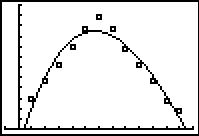
\includegraphics[width=2in]{./PolynomialsGraphics/REG3.jpg} \hspace{.25in} & 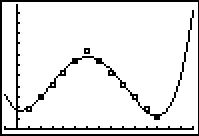
\includegraphics[width=2in]{./PolynomialsGraphics/REG4.jpg} \\

$y = p_{\mbox{\tiny $3$}}(x)$ \hspace{.25in} & $y = p_{\mbox{\tiny $4$}}(x)$ \\

\end{tabular}

\end{center}

\item \begin{enumerate}

\item The scatter plot is shown below with each of the three regression models.

\item The quadratic model is $P_{\mbox{\tiny $2$}}(x) = -0.02x^{2} + 0.241x + 0.956$ with $R^{2} = 0.77708$. \\
The cubic model is $P_{\mbox{\tiny $3$}}(x) = 0.005x^{3} - 0.103x^{2} + 0.602x + 0.573$ with $R^{2} = 0.98153$. \\
The quartic model is $P_{\mbox{\tiny $4$}}(x) = -0.000969x^{4} + 0.0253x^{3} - 0.240x^{2} + 0.944x + 0.330$ with $R^{2} = 0.99929$.

\item The maximums predicted by the three models are $P_{\mbox{\tiny $2$}}(5.737) \approx 1.648$, $P_{\mbox{\tiny $3$}}(4.232) \approx 1.657$ and $P_{\mbox{\tiny $4$}}(3.784) \approx 1.630$, respectively.

\end{enumerate}

\hspace{-.1in} \begin{tabular}{ccc}

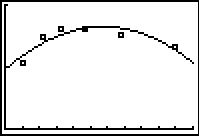
\includegraphics[width=1.8in]{./PolynomialsGraphics/CIRC2.jpg} \hspace{.1in} &
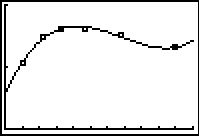
\includegraphics[width=1.8in]{./PolynomialsGraphics/CIRC3.jpg} \hspace{.1in} &
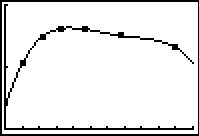
\includegraphics[width=1.8in]{./PolynomialsGraphics/CIRC4.jpg} \\

$y = P_{\mbox{\tiny $2$}}(x)$ \hspace{.1in} & $y = P_{\mbox{\tiny $3$}}(x)$ & $y = P_{\mbox{\tiny $4$}}(x)$\\

\end{tabular}

\end{enumerate}

\closegraphsfile

\newpage

\section{The Factor Theorem and the Remainder Theorem}

\mfpicnumber{1}

\opengraphsfile{Polydivision}

\setcounter{footnote}{0}

\label{Polydivision}


Suppose we wish to find the zeros of $f(x) = x^3 + 4x^2-5x-14$.  Setting $f(x)=0$ results in the polynomial equation $x^3 + 4x^2-5x-14=0$.   Despite all of the factoring techniques we learned\footnote{and probably forgot} in Intermediate Algebra, this equation foils\footnote{pun intended} us at every turn.  If we graph $f$ using the graphing calculator, we get

\smallskip

\centerline{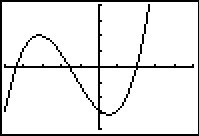
\includegraphics[width=2in]{./PolynomialsGraphics/PolyDiv01.jpg}}

\smallskip

The graph suggests that the function has three zeros, one of which is $x=2$.  It's easy to show that $f(2) = 0$, but the other two zeros seem to be less friendly.  Even though we could use the `Zero' command to find decimal approximations for these, we seek a method to find the remaining zeros \emph{exactly}.  Based on our experience, if $x=2$ is a zero, it seems that there should be a factor of $(x-2)$ lurking around in the factorization of $f(x)$.  In other words, we should expect that $x^3 + 4x^2-5x-14=(x-2) \, q(x)$, where $q(x)$ is some other polynomial.  How could we find such a $q(x)$, if it even exists?  The answer comes from our old friend, polynomial division. Dividing $x^3 + 4x^2-5x-14$ by $x-2$ gives

\setlength\arraycolsep{0.1pt}
\setlength\extrarowheight{2pt}

\[ \begin{array}{cccccccccc}

& & & & & x^2 & + & 6x & + & 7 \\ \hhline{~~~|-------}

x & - & 2 \, \vline& x^3 & + & 4x^2 & - & 5x & - & 14 \\

 &  &  -& \left(x^3 \right. & - & \left.  2x^2\right) &  &  &  &  \\ \hhline{~~~---~~~~} 
 &  &  &   &  & 6 x^2 & - & 5x &  &  \\ 
 &  &  &   & - & \left(6 x^2 \right. & - & \left. 12x \right) &  &  \\ \hhline{~~~~~---~~} 
 &  &  &   &   &  & & 7x  & - & 14 \\
 &  &  &   &   &  & - & \left( 7x \right. & - & \left. 14 \right) \\ \hhline{~~~~~~~---} 
 &   &  &  &  &  &  &  &  & 0
 
\end{array}\]

\setlength\arraycolsep{5pt}
\setlength\extrarowheight{0pt}

As you may recall, this means $x^3 + 4x^2-5x-14=(x-2)\left(x^2+6x+7\right)$, so to find the zeros of $f$, we now solve $(x-2)\left(x^2+6x+7\right)=0$.   We get $x-2=0$ (which gives us our known zero, $x=2$) as well as $x^2+6x+7=0$.   The latter doesn't factor nicely, so we apply the Quadratic Formula to get $x = -3 \pm \sqrt{2}$.  The point of this section is to generalize the technique applied here.  First up is a friendly reminder of what we can expect when we divide polynomials.

\smallskip

\colorbox{ResultColor}{\bbm

\begin{thm} \label{polydiv} \textbf{Polynomial Division:}  Suppose $d(x)$ and $p(x)$ are nonzero polynomials where the degree of $p$ is greater than or equal to the degree of $d$.  There exist two unique polynomials, $q(x)$ and $r(x)$, such that $p(x) = d(x) \, q(x) + r(x),\,$ where either $r(x) = 0$ or the degree of $r$ is strictly less than the degree of $d$.
\end{thm}
\ebm}

\smallskip

As you may recall, all of the polynomials in Theorem \ref{polydiv} have special names.  The polynomial $p$ is called the \index{polynomial division ! dividend} \textbf{dividend}; $d$ is the \index{polynomial division ! divisor} \textbf{divisor}; $q$ is the \index{polynomial division ! quotient} \textbf{quotient}; $r$ is the \index{polynomial division ! remainder} \textbf{remainder}.  If $r(x)=0$ then $d$ is called a \index{polynomial division ! factor} \textbf{factor} of $p$.  The proof of Theorem \ref{polydiv} is usually relegated to a course in Abstract Algebra,\footnote{Yes, Virginia, there are Algebra courses more abstract than this one.} but we can still use the result to establish two important facts which are the basis of the rest of the chapter.

\smallskip

\colorbox{ResultColor}{\bbm

\begin{thm} \label{remainderthm}\index{Remainder Theorem}\textbf{The Remainder Theorem:}  Suppose $p$ is a polynomial of degree at least $1$ and $c$ is a real number.  When $p(x)$ is divided by $x-c$ the remainder is $p(c)$.  

\end{thm}
\ebm}

\smallskip


The proof of Theorem \ref{remainderthm} is a direct consequence of Theorem \ref{polydiv}.  When a polynomial is divided by $x-c$, the remainder is either $0$ or has degree less than the degree of $x-c$.  Since $x-c$ is degree $1$, the degree of the remainder must be $0$, which means the remainder is a constant.  Hence, in either case, $p(x) = (x-c) \, q(x) + r$, where $r$, the remainder, is a real number, possibly $0$.  It follows that $p(c) = (c-c) \, q(c) + r = 0 \cdot q(c) + r = r$, so we get $r = p(c)$ as required.  There is one last `low hanging fruit'\footnote{Jeff hates this expression and Carl included it just to annoy him.} to collect which we present below.

\smallskip

\colorbox{ResultColor}{\bbm

\begin{thm} \label{factorthm}\index{Factor Theorem}\textbf{The Factor Theorem:}  Suppose $p$ is a nonzero polynomial.  The real number $c$ is a zero of $p$ if and only if $(x-c)$ is a factor of $p(x)$.  

\end{thm}
\ebm}

\smallskip

The proof of The Factor Theorem is a consequence of what we already know.  If $(x-c)$ is a factor of $p(x)$, this means $p(x) = (x-c) \, q(x)$ for some polynomial $q$.  Hence, $p(c) = (c-c) \, q(c) = 0$, so $c$ is a zero of $p$.  Conversely, if $c$ is a zero of $p$, then $p(c) = 0$. In this case, The Remainder Theorem tells us the remainder when $p(x)$ is divided by $(x-c)$, namely $p(c)$, is $0$, which means $(x-c)$ is a factor of $p$.  What we have established is the fundamental connection between zeros of polynomials and factors of polynomials.  

\smallskip

Of the things The Factor Theorem tells us, the most pragmatic is that we had better find a more efficient way to divide polynomials by quantities of the form $x-c$.  Fortunately, people like \href{http://en.wikipedia.org/wiki/Synthetic_division}{\underline{Ruffini}} and \href{http://en.wikipedia.org/wiki/Horner_scheme}{\underline{Horner}} have already blazed this trail.  Let's take a closer look at the long division we performed at the beginning of the section and try to streamline it.  First off, let's change all of the subtractions into additions by distributing through the $-1$s.


\setlength\arraycolsep{0.1pt}
\setlength\extrarowheight{2pt}

\[ \begin{array}{cccccccccc}

& & & & & x^2 & + & 6x & + & 7 \\ \hhline{~~~|-------}

x & - & 2 \, \vline& x^3 & + & 4x^2 & - & 5x & - & 14 \\

 &  &  &  -x^3  & + &   2x^2 &  &  &  &  \\ \hhline{~~~---~~~~} 
 &  &  &   &  & 6 x^2 & - & 5x &  &  \\ 
 &  &  &   & &-6 x^2  & + &  12x &  &  \\ \hhline{~~~~~---~~} 
 &  &  &   &   &  & & 7x  & - & 14 \\
 &  &  &   &   &  & & - 7x  & + &  14  \\ \hhline{~~~~~~~---} 
 &   &  &  &  &  &  &  &  & 0
 
\end{array}\]

\setlength\arraycolsep{5pt}
\setlength\extrarowheight{0pt}


Next, observe that the terms $-x^3$, $-6x^2$ and $-7x$ are the exact opposite of the terms above them.  The algorithm we use ensures this is always the case, so we can omit them without losing any information. Also note that the terms we `bring down' (namely the $-5x$ and $-14$) aren't really necessary to recopy, so we omit them, too.


\setlength\arraycolsep{0.1pt}
\setlength\extrarowheight{2pt}

\[ \begin{array}{cccccccccc}

& & & & & x^2 & + & 6x & + & 7 \\ \hhline{~~~|-------}

x & - & 2 \, \vline& \, \, x^3 & + & 4x^2 & - & 5x & - & 14 \\

 &  &  &   &  &   2x^2 &  &  &  &  \\ \hhline{~~~---~~~~} 
 &  &  &   &  & 6 x^2 &  &  &  &  \\ 
 &  &  &   & &  &  &  12x &  &  \\ \hhline{~~~~~---~~} 
 &  &  &   &   &  & & 7x  &  &  \\
 &  &  &   &   &  & &   &  &  14  \\ \hhline{~~~~~~~---} 
 &   &  &  &  &  &  &  &  & 0
 
\end{array}\]

\setlength\arraycolsep{5pt}
\setlength\extrarowheight{0pt}

Now, let's move things up a bit and, for reasons which will become clear in a moment, copy the $x^3$ into the last row.


\setlength\arraycolsep{0.1pt}
\setlength\extrarowheight{2pt}

\[ \begin{array}{cccccccccc}

& & & & & x^2 & + & 6x & + & 7 \\ \hhline{~~~|-------}

x & - & 2 \, \vline& \, \, x^3 & + & 4x^2 & - & 5x & - & 14 \\

 &  &  &   & &   2x^2 &  & 12x &  & 14 \\ \hhline{~~~-------} 
 &  &  & x^3  &  & 6 x^2 &  & 7x &  &0  \\  
\end{array}\]

\setlength\arraycolsep{5pt}
\setlength\extrarowheight{0pt}

Note that by arranging things in this manner, each term in the last row is obtained by adding the two terms above it.  Notice also that the quotient polynomial can be obtained by dividing each of the first three terms in the last row by $x$ and adding the results.   If you take the time to work back through the original division problem, you will find that this is exactly the way we determined the quotient polynomial.  This means that we no longer need to write the quotient polynomial down, nor the $x$ in the divisor, to determine our answer.

\setlength\arraycolsep{0.1pt}
\setlength\extrarowheight{2pt}

\[ \begin{array}{cccccccccc}


 & & - 2 \, \, \vline& \, \, x^3 & + & 4x^2 & - & 5x & - & 14 \\

 &  &  &   & &   2x^2 &  & 12x &  & 14 \\ \hhline{~~~-------} 
 &  &  & x^3  &  & 6 x^2 &  & 7x &  &0  \\  
\end{array}\]

\setlength\arraycolsep{5pt}
\setlength\extrarowheight{0pt}

We've streamlined things quite a bit so far, but we can still do more.  Let's take a moment to remind ourselves where the $2x^2$, $12x$ and $14$ came from in the second row.  Each of these terms was obtained by multiplying the terms in the quotient, $x^2$, $6x$ and $7$, respectively, by the $-2$ in $x-2$,  then by $-1$ when we changed the subtraction to addition.  Multiplying by $-2$ then by $-1$ is the same as multiplying by $2$, so we replace the $-2$ in the divisor by $2$.   Furthermore, the coefficients of the quotient polynomial match the coefficients of the first three terms in the last row, so we now take the plunge and write only the coefficients of the terms to get



\[ \begin{array}{rrrrr}


  2 \, \, \vline& 1 & 4 & -5  & -14 \\

   &&   2 &   12 &   14 \\ \hhline{~----} 
  & 1  &   6  &  7 &  0  \\  
\end{array}\]



We have constructed a \index{polynomial division ! synthetic division}\index{synthetic division tableau}\textbf{synthetic division tableau} for this polynomial division problem.  Let's re-work our division problem using this tableau to see how it greatly streamlines the division process.  To divide $x^3+4x^2-5x-14$ by $x-2$, we write $2$ in the place of the divisor and the coefficients of $x^3+4x^2-5x-14$ in for the dividend.  Then `bring down' the first coefficient of the dividend.

\bigskip

\begin{center}

\begin{tabular}{cc}

$ \begin{array}{rrrrr}


  2 \, \, \vline& 1 & 4 & -5  & -14 \\

   &  &    &    &  \\ \hhline{~----} 
  &   &     &   &    \\  
\end{array}$  \hspace{1in}
&


$ \begin{array}{rrrrr}


  2 \, \, \vline& 1 & 4 & -5  & -14 \\

   & \downarrow &    &    &  \\ \hhline{~----} 
  & 1  &     &   &    \\  
\end{array}$ \\

\end{tabular}

\end{center}

\bigskip

Next, take the $2$ from the divisor and multiply by the $1$ that was `brought down' to get $2$.  Write this underneath the $4$, then add to get $6$.

\bigskip

\begin{center}

\begin{tabular}{cc}

$ \begin{array}{rrrrr}


  2 \, \, \vline& 1 & 4 & -5  & -14 \\

   & \downarrow  &  2  &    &  \\ \hhline{~----} 
  & 1  &     &   &    \\  
\end{array}$ \hspace{1in}
&


$ \begin{array}{rrrrr}


  2 \, \, \vline& 1 & 4 & -5  & -14 \\

   & \downarrow &  2  &    &  \\ \hhline{~----} 
  & 1  &   6  &   &    \\  
\end{array}$ \\


\end{tabular}

\end{center}

\bigskip

Now take the $2$ from the divisor times the $6$ to get $12$, and add it to the $-5$ to get $7$.

\bigskip

\begin{center}

\begin{tabular}{cc}


$ \begin{array}{rrrrr}


  2 \, \, \vline& 1 & 4 & -5  & -14 \\

   & \downarrow &  2  &  12  &  \\ \hhline{~----} 
  & 1  &   6  &   &    \\  
\end{array}$ \hspace{1in}

&

$ \begin{array}{rrrrr}


  2 \, \, \vline& 1 & 4 & -5  & -14 \\

   & \downarrow &  2  &  12  &  \\ \hhline{~----} 
  & 1  &   6  & 7  &    \\  
\end{array}$ \\


\end{tabular}

\end{center}


Finally, take the $2$ in the divisor times the $7$ to get $14$, and add it to the $-14$ to get $0$.

\bigskip

\begin{center}

\begin{tabular}{cc}

$ \begin{array}{rrrrr}


  2 \, \, \vline& 1 & 4 & -5  & -14 \\

   & \downarrow &  2  &  12  & 14 \\ \hhline{~----} 
  & 1  &   6  & 7  &    \\  
\end{array}$ \hspace{1in} 

&

$ \begin{array}{rrrrr}


  2 \, \, \vline& 1 & 4 & -5  & -14 \\

   & \downarrow &  2  &  12  & 14 \\ \hhline{~----} 
  & 1  &   6  & 7  &  \fbox{$0$}  \\  
\end{array}$ \\



\end{tabular}

\end{center}

The first three numbers in the last row of our tableau are the coefficients of the quotient polynomial.  Remember, we started with a third degree polynomial and divided by a first degree polynomial, so the quotient is a second degree polynomial.  Hence the quotient is $x^2+6x+7$.  The number in the box is the remainder.  Synthetic division is our tool of choice for dividing polynomials by divisors of the form $x-c$.  It is important to note that it works \emph{only} for these kinds of divisors.\footnote{You'll need to use good old-fashioned polynomial long division for divisors of degree larger than 1.} Also take note that when a polynomial (of degree at least $1$) is divided by $x-c$, the result will be a polynomial of exactly one less degree. Finally, it is  worth the time to trace each step in synthetic division back to its corresponding step in long division.  While the authors have done their best to indicate where the algorithm comes from, there is no substitute for working through it yourself.

\begin{ex}  Use synthetic division to perform the following polynomial divisions.  Find the quotient and the remainder polynomials, then write the dividend, quotient and remainder in the form given in Theorem \ref{polydiv}.

\begin{multicols}{3}
\begin{enumerate}

\item  $\left(5x^3 - 2x^2 + 1\right) \div (x-3)$ \vphantom{$\dfrac{4-8x-12x^2}{2x-3}$}
\item  $\left(x^3+8\right) \div (x+2)$ \vphantom{$\dfrac{4-8x-12x^2}{2x-3}$}
\item  $\dfrac{4-8x-12x^2}{2x-3}$

\end{enumerate}
\end{multicols}

{ \bf Solution.} 

\begin{enumerate}


\item When setting up the synthetic division tableau, we need to enter $0$ for the coefficient of $x$ in the dividend.  Doing so gives


\[ \begin{array}{rrrrr}


  3 \, \, \vline& 5 & -2 & 0  & 1 \\

   & \downarrow &  15  &  39  & 117 \\ \hhline{~----} 
  & 5  &   13  & 39  &  \fbox{$118$}  \\  
\end{array}\]

Since the dividend was a third degree polynomial, the quotient is a quadratic polynomial with coefficients $5$, $13$ and $39$.  Our quotient is $q(x) = 5x^2+13x+39$ and the remainder is $r(x) = 118$.  According to Theorem \ref{polydiv}, we have $5x^3 - 2x^2 + 1 = (x-3)\left(5x^2+13x+39 \right) + 118$.

\item  For this division, we rewrite $x+2$ as $x-(-2)$ and proceed as before

\[ \begin{array}{rrrrr}


  -2 \, \, \vline& 1 & 0 & 0  & 8 \\

   & \downarrow &  -2  &  4  & -8 \\ \hhline{~----} 
  & 1  &   -2  & 4  &  \fbox{$0$}  \\  
\end{array}\]

We get the quotient $q(x) = x^2-2x+4$ and the remainder $r(x) =0$. Relating the dividend, quotient and remainder gives $x^3+8 = (x+2)\left( x^2-2x+4 \right)$.  

\item To divide $4-8x-12x^2$ by $2x-3$, two things must be done.  First, we write the dividend in descending powers of $x$ as $-12x^2-8x+4$.  Second, since synthetic division works only for factors of the form $x-c$, we factor $2x-3$ as $2\left(x-\frac{3}{2}\right)$.  Our strategy is to first divide $-12x^2-8x+4$ by $2$, to get $-6x^2-4x+2$.  Next, we divide by $\left(x-\frac{3}{2}\right)$.  The tableau becomes

\[ \begin{array}{rrrr}


  \frac{3}{2} \, \, \vline& -6 & -4 & 2   \\ [4pt]

   & \downarrow &  -9  & -\frac{39}{2}  \\ [4pt] \hhline{~---} 
  &  -6  &   -13  & \fbox{$-\frac{35}{2}$}  \\  
\end{array}\]


\end{enumerate}

From this, we get $-6x^2-4x+2 = \left(x-\frac{3}{2}\right)(-6 x - 13) - \frac{35}{2}$.  Multiplying both sides by $2$ and distributing gives $-12x^2-8x+4 = \left(2x-3\right) (-6 x - 13) - 35$.  At this stage, we have written $-12x^2-8x+4$ in the \textbf{form} $(2x-3) q(x) + r(x)$, but how can we be sure the quotient polynomial is $-6x-13$ and the remainder is $-35$?  The answer is the word `unique' in Theorem \ref{polydiv}.  The theorem states that there is only one way to decompose $-12x^2-8x+4$ into a multiple of $(2x-3)$  plus a constant term.  Since we have found such a way, we can be sure it is the only way. \qed


\end{ex}

The next example pulls together all of the concepts discussed in this section.  

\begin{ex} Let $p(x) = 2x^3-5x+3$.

\begin{enumerate}

\item  Find $p(-2)$ using The Remainder Theorem.  Check your answer by substitution.

\item  Use the fact that $x=1$ is a zero of $p$ to factor $p(x)$ and then find all of the real zeros of $p$.

\end{enumerate}

{\bf Solution.}

\begin{enumerate}

\item  The Remainder Theorem states $p(-2)$ is the remainder when $p(x)$ is divided by $x-(-2)$.  We set up our synthetic division tableau below.  We are careful to record the coefficient of $x^2$ as $0$, and proceed as above.

\[\begin{array}{rrrrr}
 -2 \, \, \vline& 2 & 0 & -5  & 3 \\

   & \downarrow &  -4  &  8  & -6 \\ \hhline{~----} 
  & 2  &   -4  & 3 &  \fbox{$-3$}  \\  
\end{array}\]

According to the Remainder Theorem, $p(-2) = -3$.  We can check this by direct substitution into the formula for $p(x)$:  $p(-2) = 2(-2)^3-5(-2)+3 = -16+10+3=-3$.

\item The Factor Theorem tells us that since $x=1$ is a zero of $p$, $x-1$ is a factor of $p(x)$.  To factor $p(x)$, we divide

\[\begin{array}{rrrrr}
 1 \, \, \vline& 2 & 0 & -5  & 3 \\

   & \downarrow &  2  &  2  & -3 \\ \hhline{~----} 
  & 2  &   2  & -3 &  \fbox{$0$}  \\  
\end{array}\]

We get a remainder of $0$ which verifies that, indeed, $p(1) = 0$.  Our quotient polynomial is a second degree polynomial with coefficients $2$, $2$, and $-3$. So $q(x) = 2x^2 + 2x - 3$.  Theorem \ref{polydiv} tells us $p(x) = (x-1)\left( 2x^2 + 2x - 3\right)$.  To find the remaining real zeros of $p$, we need to solve $2x^2 + 2x - 3=0$ for $x$.  Since this doesn't factor nicely, we use the quadratic formula to find that the remaining zeros are $x = \frac{-1 \pm \sqrt{7}}{2}$. \qed
\end{enumerate}
\end{ex}

In Section \ref{GraphsofPolynomials}, we discussed the notion of the multiplicity of a zero.  Roughly speaking, a zero with multiplicity $2$ can be divided twice into a polynomial;  multiplicity $3$, three times and so on.  This is illustrated in the next example.

\begin{ex}  Let $p(x) = 4x^4-4x^3-11x^2+12x-3$.  Given that $x=\frac{1}{2}$ is a zero of multiplicity $2$,  find all of the real zeros of $p$.

\smallskip

{\bf Solution.}  We set up for synthetic division.  Since we are told the multiplicity of $\frac{1}{2}$ is two, we continue our tableau and divide $\frac{1}{2}$ into the quotient polynomial

\[\begin{array}{rrrrrr}
 \frac{1}{2} \, \, \vline& 4 & -4 & -11  & 12 & -3 \\

   & \downarrow &  2  &  -1  & -6 & 3\\ \hhline{~-----} 
   
  \frac{1}{2} \, \, \vline&  4  &   -2  & -12 & 6 &  \fbox{$0$}  \\
    
      & \downarrow &  2  &  0  & -6 &\\ \hhline{~----} 
      
       & 4  &   0  & -12 & \fbox{0} &   \\  



\end{array}\]

From the first division, we get $4x^4-4x^3-11x^2+12x-3=\left(x-\frac{1}{2}\right) \left(4x^3-2x^2-12x+6\right)$.  The second division tells us $4x^3-2x^2-12x+6=\left(x-\frac{1}{2}\right)\left(4x^2-12\right)$.  Combining these results, we have  $4x^4-4x^3-11x^2+12x-3 = \left(x-\frac{1}{2}\right)^2\left(4x^2-12\right)$.  To find the remaining zeros of $p$, we set $4x^2-12=0$ and get $x = \pm \sqrt{3}$.  \qed

\end{ex}

A couple of things about the last example are worth mentioning. First, the extension of the synthetic division tableau for repeated divisions will be a common site in the sections to come. Typically, we will start with a higher order polynomial and peel off one zero at a time until we are left with a quadratic, whose roots can always be found using the Quadratic Formula.  Secondly, we found $x = \pm \sqrt{3}$ are zeros of $p$.  The Factor Theorem guarantees $\left(x-\sqrt{3}\right)$ and $\left(x - \left(-\sqrt{3}\right)\right)$ are both factors of $p$.  We can certainly put the Factor Theorem to the test and continue the synthetic division tableau from above to see what happens.

\[\begin{array}{rrrrrr}
 \frac{1}{2} \, \, \vline& 4 & -4 & -11  & 12 & -3 \\

  & \downarrow &  2  &  -1  & -6 & 3\\ \hhline{~-----} 
  
  \frac{1}{2} \, \, \vline&  4  &   -2  & -12 & 6 &  \fbox{$0$}  \\
    
  & \downarrow &  2  &  0  & -6 &\\ \hhline{~----} 
 
  
 \sqrt{3} \, \, \vline  & 4  &   0  & -12 & \fbox{0} &   \\
  
                        & \downarrow &  4\sqrt{3}  & 12  & &\\ \hhline{~---} 
 
   -\sqrt{3} \, \, \vline  & 4  &  4\sqrt{3}  & \fbox{0} &  &   \\  
       
                          & \downarrow &  -4\sqrt{3}  &   & &\\ \hhline{~--} 
       
													& 4  &  \fbox{0}  &  &  &   \\

\end{array}\]

This gives us $4x^4-4x^3-11x^2+12x-3=\left(x-\frac{1}{2}\right)^2 \left(x-\sqrt{3}\right)\left(x - \left(-\sqrt{3}\right)\right) (4)$, or, when written with the constant in front \[ p(x) = 4\left(x-\frac{1}{2}\right)^2 \left(x-\sqrt{3}\right)\left(x - \left(-\sqrt{3}\right)\right)\]

We have shown that $p$ is a product of its leading coefficient times linear factors of the form $(x-c)$ where $c$ are zeros of $p$. It may surprise and delight the reader that, in theory, all polynomials can be reduced to this kind of factorization.  We leave that discussion to Section \ref{ComplexZeros}, because the zeros may not be real numbers.  Our final theorem in the section gives us an upper bound on the number of real zeros. 

\medskip

\colorbox{ResultColor}{\bbm
\begin{thm}  \label{nzerosreal} Suppose $f$ is a polynomial of degree $n \geq 1$.  Then $f$ has at most $n$ real zeros, counting multiplicities.

\end{thm}
\ebm}

\medskip

Theorem \ref{nzerosreal} is a consequence of the Factor Theorem and polynomial multiplication.  Every zero $c$ of $f$ gives us a factor of the form $(x-c)$ for $f(x)$.  Since $f$ has degree $n$, there can be at most $n$ of these factors.  The next section provides us some tools which not only help us determine where the real zeros are to be found, but which real numbers they may be.

\medskip

We close this section with a summary of several concepts previously presented.  You should take the time to look back through the text to see where each concept was first introduced and where each connection to the other concepts was made.

\medskip

\colorbox{ResultColor}{\bbm

\centerline{\textbf{Connections Between Zeros, Factors and Graphs of Polynomial Functions}}

\medskip

\hspace{.17in} Suppose $p$ is a polynomial function of degree $n \geq 1$.  The following statements are equivalent:

\begin{itemize}

\item The real number $c$ is a zero of $p$
\item $p(c) = 0$
\item $x = c$ is a solution to the polynomial equation $p(x) = 0$
\item $(x - c)$ is a factor of $p(x)$
\item The point $(c, 0)$ is an $x$-intercept of the graph of $y = p(x)$

\end{itemize}

\ebm}

\newpage

\subsection{Exercises}

In Exercises \ref{polydivreviewfirst} - \ref{polydivreviewlast}, use polynomial long division to perform the indicated division.  Write the polynomial in the form $p(x) = d(x)q(x) + r(x)$.

\begin{multicols}{2}
\begin{enumerate}

\item $\left(4x^2+3x-1 \right) \div (x-3)$ \label{polydivreviewfirst}
\item $\left(2x^3-x+1 \right) \div \left(x^{2} +x+1 \right)$ 

\setcounter{HW}{\value{enumi}}
\end{enumerate}
\end{multicols}

\begin{multicols}{2}
\begin{enumerate}
\setcounter{enumi}{\value{HW}}

\item $\left(5x^{4} - 3x^{3} + 2x^{2} - 1 \right) \div \left(x^{2} + 4 \right)$
\item $\left(-x^{5} + 7x^{3} - x \right) \div \left(x^{3} - x^{2} + 1 \right)$

\setcounter{HW}{\value{enumi}}
\end{enumerate}
\end{multicols}

\begin{multicols}{2}
\begin{enumerate}
\setcounter{enumi}{\value{HW}}

\item $\left(9x^{3} + 5 \right) \div \left(2x - 3 \right)$
\item $\left(4x^2 - x - 23 \right) \div \left(x^{2} - 1 \right)$ \label{polydivreviewlast}

\setcounter{HW}{\value{enumi}}
\end{enumerate}
\end{multicols}

In Exercises \ref{synthdivreviewfirst} - \ref{synthdivreviewlast} use synthetic division to perform the indicated division.  Write the polynomial in the form $p(x) = d(x)q(x) + r(x)$.

\begin{multicols}{2}
\begin{enumerate}
\setcounter{enumi}{\value{HW}}

\item $\left(3x^2-2x+1 \right) \div \left(x-1\right)$ \label{synthdivreviewfirst}
\item $\left(x^2-5 \right) \div \left(x-5\right)$

\setcounter{HW}{\value{enumi}}
\end{enumerate}
\end{multicols}

\begin{multicols}{2}
\begin{enumerate}
\setcounter{enumi}{\value{HW}}

\item $\left(3-4x-2x^2 \right) \div \left(x+1\right)$
\item $\left(4x^2-5x +3\right) \div \left(x+3\right)$

\setcounter{HW}{\value{enumi}}
\end{enumerate}
\end{multicols}

\begin{multicols}{2}
\begin{enumerate}
\setcounter{enumi}{\value{HW}}

\item $\left(x^3 + 8 \right) \div \left(x+2\right)$
\item $\left(4x^3 +2x-3 \right) \div \left(x -3\right)$

\setcounter{HW}{\value{enumi}}
\end{enumerate}
\end{multicols}

\begin{multicols}{2}
\begin{enumerate}
\setcounter{enumi}{\value{HW}}

\item $\left(18x^2-15x-25\right) \div \left(x - \frac{5}{3} \right)$
\item $\left(4x^2-1 \right) \div \left(x - \frac{1}{2} \right)$

\setcounter{HW}{\value{enumi}}
\end{enumerate}
\end{multicols}

\begin{multicols}{2}
\begin{enumerate}
\setcounter{enumi}{\value{HW}}

\item $\left(2x^3+x^2+2x+1 \right) \div \left(x + \frac{1}{2} \right)$
\item $\left(3x^3 - x + 4 \right) \div \left(x - \frac{2}{3} \right)$

\setcounter{HW}{\value{enumi}}
\end{enumerate}
\end{multicols}

\begin{multicols}{2}
\begin{enumerate}
\setcounter{enumi}{\value{HW}}

\item $\left(2x^3 - 3x +1 \right) \div \left(x - \frac{1}{2} \right)$
\item $\left(4x^4-12x^3+13x^2 -12x+9\right) \div \left(x - \frac{3}{2} \right)$

\setcounter{HW}{\value{enumi}}
\end{enumerate}
\end{multicols}

\begin{multicols}{2}
\begin{enumerate}
\setcounter{enumi}{\value{HW}}

\item $\left(x^4-6x^2+9 \right) \div \left(x -\sqrt{3} \right)$
\item $\left(x^6-6x^4+12x^2-8\right) \div \left(x +\sqrt{2} \right)$ \label{synthdivreviewlast}

\setcounter{HW}{\value{enumi}}
\end{enumerate}
\end{multicols}

In Exercises \ref{remainderexerfirst} - \ref{remainderexerlast}, determine $p(c)$ using the Remainder Theorem for the given polynomial functions and value of $c$.  If $p(c) = 0$, factor $p(x) = (x-c) q(x)$.

\begin{multicols}{2}
\begin{enumerate}
\setcounter{enumi}{\value{HW}}

\item $p(x) = 2x^2 - x + 1$, $c = 4$ \label{remainderexerfirst}
\item $p(x) = 4x^2-33x-180$, $c = 12$

\setcounter{HW}{\value{enumi}}
\end{enumerate}
\end{multicols}


\begin{multicols}{2}
\begin{enumerate}
\setcounter{enumi}{\value{HW}}

\item $p(x) = 2x^3 - x + 6$, $c=-3$
\item $p(x) = x^3+2x^2+3x+4$, $c =-1$

\setcounter{HW}{\value{enumi}}
\end{enumerate}
\end{multicols}

\begin{multicols}{2}
\begin{enumerate}
\setcounter{enumi}{\value{HW}}

\item $p(x) =3x^3-6x^2+4x-8$, $c=2$
\item $p(x) = 8x^3+12x^2+6x+1$, $c =-\frac{1}{2}$

\setcounter{HW}{\value{enumi}}
\end{enumerate}
\end{multicols}

\begin{multicols}{2}
\begin{enumerate}
\setcounter{enumi}{\value{HW}}

\item $p(x) = x^4 - 2x^2+4$, $c=\frac{3}{2}$
\item $p(x) = 6x^4-x^2+2$, $c =-\frac{2}{3}$

\setcounter{HW}{\value{enumi}}
\end{enumerate}
\end{multicols}


\begin{multicols}{2}
\begin{enumerate}
\setcounter{enumi}{\value{HW}}

\item $p(x) = x^4 +x^3-6x^2-7x-7$, $c=-\sqrt{7}$
\item $p(x) = x^2-4x+1$, $c =2-\sqrt{3}$ \label{remainderexerlast}

\setcounter{HW}{\value{enumi}}
\end{enumerate}
\end{multicols}

\newpage

In Exercises \ref{factorpolyzerofirst} - \ref{factorpolyzerolast}, you are given a polynomial and one of its zeros.  Use the techniques in this section to find the rest of the real zeros and factor the polynomial.  

\begin{multicols}{2}
\begin{enumerate}
\setcounter{enumi}{\value{HW}}

\item $x^{3} - 6x^{2} + 11x - 6, \;\; c = 1$ \label{factorpolyzerofirst}
\item $x^{3} - 24x^{2} + 192x - 512, \;\; c = 8$

\setcounter{HW}{\value{enumi}}
\end{enumerate}
\end{multicols}

\begin{multicols}{2}
\begin{enumerate}
\setcounter{enumi}{\value{HW}}

\item $3x^{3} + 4x^{2} - x - 2, \;\; c = \frac{2}{3}$
\item $2x^3-3x^2-11x+6, \;\; c=\frac{1}{2}$

\setcounter{HW}{\value{enumi}}
\end{enumerate}
\end{multicols}

\begin{multicols}{2}
\begin{enumerate}
\setcounter{enumi}{\value{HW}}

\item $x^3+2x^2-3x-6, \;\; c = -2$
\item $2x^3-x^2-10x+5, \;\; c=\frac{1}{2}$

\setcounter{HW}{\value{enumi}}
\end{enumerate}
\end{multicols}


\begin{enumerate}
\setcounter{enumi}{\value{HW}}

\item $4x^{4} - 28x^{3} + 61x^{2} - 42x + 9$, $c = \frac{1}{2}$ is a zero of multiplicity 2 

\item  $x^5+2x^4-12x^3-38x^2-37x-12$, $c=-1$ is a zero of multiplicity 3

\item $125x^{5} - 275x^{4} - 2265x^{3} - 3213x^{2} - 1728x - 324$, $c = -\frac{3}{5}$ is a zero of multiplicity 3

\item $x^{2} - 2x - 2, \;\; c = 1 - \sqrt{3}$ \label{factorpolyzerolast}

\setcounter{HW}{\value{enumi}}
\end{enumerate}

In Exercises \ref{buildapolyexerfirst} - \ref{buildapolyexerlast}, create a polynomial $p$ which has the desired characteristics.  You may leave the polynomial in factored form. 

\begin{enumerate}
\setcounter{enumi}{\value{HW}}

\item \label{buildapolyexerfirst}

\begin{itemize}

\item The zeros of $p$ are $c = \pm 2$ and $c = \pm 1$
\item The leading term of $p(x)$ is $117x^4$.

\end{itemize}

\item

\begin{itemize}

\item The zeros of $p$ are $c=1$ and $c = 3$
\item $c=3$ is a zero of multiplicity 2.
\item The leading term of $p(x)$ is $-5x^3$

\end{itemize}

\item

\begin{itemize}

\item The solutions to $p(x) = 0$ are $x = \pm 3$ and $x=6$
\item The leading term of $p(x)$ is $7x^4$
\item The point $(-3,0)$ is a local minimum on the graph of $y=p(x)$.

\end{itemize}


\item

\begin{itemize}

\item The solutions to $p(x) =0$ are $x = \pm 3$, $x=-2$, and $x=4$.
\item The leading term of $p(x)$ is $-x^5$.
\item The point $(-2, 0)$ is a local maximum on the graph of $y=p(x)$.

\end{itemize}

\item \label{buildapolyexerlast}

\begin{itemize}

\item $p$ is degree 4.
\item as $x \rightarrow \infty$, $p(x) \rightarrow -\infty$
\item $p$ has exactly three $x$-intercepts:  $(-6,0)$, $(1,0)$ and $(117,0)$
\item  The graph of $y=p(x)$ crosses through the $x$-axis at $(1,0)$.

\end{itemize}



\item Find a quadratic polynomial with \underline{integer} coefficients which has $x = \dfrac{3}{5} \pm \dfrac{\sqrt{29}}{5}$ as its real zeros.

\end{enumerate}

\newpage

\subsection{Answers}


\begin{enumerate}

\item $4x^2+3x-1 = (x-3)(4x+15) + 44$
\item $2x^3-x+1 = \left(x^2+x+1\right)(2x-2)+(-x+3)$
\item $5x^{4} - 3x^{3} + 2x^{2} - 1 = \left(x^{2} + 4 \right) \left(5x^{2} - 3x - 18 \right) + (12x + 71)$
\item $-x^{5} + 7x^{3} - x = \left(x^{3} - x^{2} + 1 \right) \left(-x^{2} - x + 6 \right) + \left(7x^{2} - 6 \right)$
\item $9x^{3} + 5 =(2x - 3) \left(\frac{9}{2}x^{2} + \frac{27}{4}x + \frac{81}{8} \right) + \frac{283}{8}$
\item $4x^2 - x - 23 = \left(x^{2} - 1 \right)(4) + (-x - 19)$


\item $\left(3x^2-2x+1 \right) = \left(x-1\right) (3x+1)+2$
\item $\left(x^2-5 \right)= \left(x-5\right)(x+5) + 20$


\item $\left(3-4x-2x^2 \right) = \left(x+1\right)(-2x-2)+5$
\item $\left(4x^2-5x +3\right) = \left(x+3\right)(4x-17)+54$


\item $\left(x^3 + 8 \right) = \left(x+2\right) \left(x^2-2x+4\right) + 0$
\item $\left(4x^3 +2x-3 \right) = \left(x -3\right) \left(4x^2+12x+38\right) + 111$


\item $\left(18x^2-15x-25\right) = \left(x - \frac{5}{3} \right)(18x+15)+0$
\item $\left(4x^2-1 \right) = \left(x - \frac{1}{2} \right)(4x+2)+0$


\item $\left(2x^3+x^2+2x+1 \right) = \left(x + \frac{1}{2} \right)\left(2x^2+2\right)+0$
\item $\left(3x^3 - x + 4 \right) = \left(x - \frac{2}{3} \right) \left(3x^2+2x+\frac{1}{3}\right) + \frac{38}{9}$


\item $\left(2x^3 - 3x +1 \right) = \left(x - \frac{1}{2} \right) \left(2x^2+x-\frac{5}{2}\right)-\frac{1}{4}$
\item $\left(4x^4-12x^3+13x^2 -12x+9\right) = \left(x - \frac{3}{2} \right) \left(4x^3-6x^2+4x-6 \right)+0$

\item $\left(x^4-6x^2+9 \right) = \left(x -\sqrt{3} \right) \left(x^3+\sqrt{3} \,x^2-3x-3\sqrt{3}\right) + 0$
\item $\left(x^6-6x^4+12x^2-8\right) = \left(x +\sqrt{2} \right) \left(x^5-\sqrt{2} \, x^4-4x^3+4\sqrt{2} \, x^2+4x-4\sqrt{2}\right) + 0$


\setcounter{HW}{\value{enumi}}
\end{enumerate}

\begin{multicols}{2}
\begin{enumerate}
\setcounter{enumi}{\value{HW}}

\item $p(4) = 29$
\item $p(12) =0$, $p(x) = (x-12)(4x+15)$

\setcounter{HW}{\value{enumi}}
\end{enumerate}
\end{multicols}


\begin{multicols}{2}
\begin{enumerate}
\setcounter{enumi}{\value{HW}}

\item $p(-3)=-45$
\item $p(-1)=2$

\setcounter{HW}{\value{enumi}}
\end{enumerate}
\end{multicols}

\begin{multicols}{2}
\begin{enumerate}
\setcounter{enumi}{\value{HW}}

\item $p(2) =0$, $p(x)= (x-2) \left(3x^2+4\right)$
\item $p\left(-\frac{1}{2}\right) = 0$, $p(x)  = \left(x+\frac{1}{2}\right)\left(8x^2+8x+2\right)$

\setcounter{HW}{\value{enumi}}
\end{enumerate}
\end{multicols}

\begin{multicols}{2}
\begin{enumerate}
\setcounter{enumi}{\value{HW}}

\item $p\left(\frac{3}{2}\right) = \frac{73}{16}$
\item $p\left(-\frac{2}{3}\right) = \frac{74}{27}$

\setcounter{HW}{\value{enumi}}
\end{enumerate}
\end{multicols}

\begin{enumerate}
\setcounter{enumi}{\value{HW}}

\item $p(-\sqrt{7}) = 0$, $p(x) = (x+\sqrt{7})\left(x^3+(1-\sqrt{7}) x^2+(1-\sqrt{7})x-\sqrt{7}  \right)$
\item $p(2-\sqrt{3}) =0$, $p(x) = (x-(2-\sqrt{3}))(x-(2+\sqrt{3})) $

\setcounter{HW}{\value{enumi}}
\end{enumerate}

\begin{enumerate}
\setcounter{enumi}{\value{HW}}

\item $x^{3} - 6x^{2} + 11x - 6 = (x - 1)(x - 2)(x - 3)$
\item $x^{3} - 24x^{2} + 192x - 512 = (x - 8)^{3}$
\item $3x^{3} + 4x^{2} - x - 2 = 3\left(x - \frac{2}{3}\right)(x + 1)^{2}$

\item $2x^3-3x^2-11x+6 = 2\left(x-\frac{1}{2}\right)(x+2)(x-3)$

\item $x^3+2x^2-3x-6 = (x+2)(x+\sqrt{3})(x-\sqrt{3})$
\item $2x^3-x^2-10x+5=2\left(x-\frac{1}{2}\right)(x+\sqrt{5})(x-\sqrt{5})$

\item $4x^{4} - 28x^{3} + 61x^{2} - 42x + 9 = 4\left(x - \frac{1}{2} \right)^{2}(x - 3)^{2}$

\item  $x^5+2x^4-12x^3-38x^2-37x-12 = (x+1)^3(x+3)(x-4)$

\item $125x^{5} - 275x^{4} - 2265x^{3} - 3213x^{2} - 1728x - 324$ = $125\left(x + \frac{3}{5} \right)^{3}(x + 2)(x - 6)$


\item $x^{2} - 2x - 2 = (x - (1 - \sqrt{3}))(x - (1 + \sqrt{3}))$

\setcounter{HW}{\value{enumi}}
\end{enumerate}

\begin{enumerate}
\setcounter{enumi}{\value{HW}}

\item $p(x) = 117(x+2)(x-2)(x+1)(x-1)$

\item $p(x)= -5(x-1)(x-3)^2$

\item  $p(x) = 7(x+3)^2(x-3)(x-6)$

\item $p(x) = -(x + 2)^{2}(x - 3)(x + 3)(x - 4)$

\item $p(x) = a(x+6)^2(x-1)(x-117)$ or $p(x) = a(x+6)(x-1)(x-117)^{2}$ where $a$ can be any negative real number

\item $p(x) = 5x^{2} - 6x - 4$


\end{enumerate}

\closegraphsfile

\newpage

\section{Real Zeros of Polynomials}

\mfpicnumber{1}

\opengraphsfile{RealZeros_New}

\setcounter{footnote}{0}

\label{RealZeros}

In Section \ref{Polydivision}, we found that we can use synthetic division to determine if a given real number is a zero of a polynomial function.  This section presents results which will help us determine good candidates to test using synthetic division.  There are two approaches to the topic of finding the real zeros of a polynomial.  The first approach (which is gaining popularity) is to use a little bit of Mathematics followed by a good use of technology like graphing calculators.  The second approach (for purists) makes good use of mathematical machinery (theorems) only.  For completeness, we include the two approaches but in separate subsections.\footnote{Carl is the purist and is responsible for all of the theorems in this section.  Jeff, on the other hand, has spent too much time in school politics and has been polluted with notions of `compromise.'  You can blame the slow decline of civilization on him and those like him who mingle Mathematics with technology.}  Both approaches benefit from the following two theorems, the first of which is due to the famous mathematician \href{http://en.wikipedia.org/wiki/Cauchy}{\underline{Augustin Cauchy}}.  It gives us an interval on which all of the real zeros of a polynomial can be found.

\smallskip

\colorbox{ResultColor}{\bbm

\begin{thm} \label{CauchysBound}\index{Cauchy's Bound}\textbf{Cauchy's Bound:}  Suppose $f(x) = a_{n} x^{n} + a_{n-\mbox{\tiny$1$}}x^{n-\mbox{\tiny$1$}} + \ldots + a_{\mbox{\tiny$1$}} x + a_{\mbox{\tiny$0$}}$ is a polynomial of degree $n$ with $n \geq 1$.  Let $M$ be the largest of the numbers: $\frac{|a_{0}|}{|a_{n}|}$, $\frac{|a_{1}|}{|a_{n}|}$, \ldots, $\frac{|a_{n-1}|}{|a_{n}|}$.  Then all the real zeros of $f$ lie in in the interval $[-(M+1),M+1]$.
\end{thm}

\ebm}

\smallskip

The proof of this fact is not easily explained within the confines of this text.  This \href{http://titan.princeton.edu/papers/claire/hertz-etal-99.ps}{\underline{paper}} contains the result and gives references to its proof. Like many of the results in this section, Cauchy's Bound is best understood with an example.

\begin{ex} \label{CBex} Let $f(x) = 2x^4+4x^3-x^2-6x-3$.  Determine an interval which contains all of the real zeros of $f$.

\smallskip

{\bf Solution.} To find the $M$ stated in Cauchy's Bound, we take the absolute value of the leading coefficient, in this case $|2| = 2$ and divide it into the largest (in absolute value) of the remaining coefficients, in this case $|-6| = 6$.   This yields $M=3$ so it is guaranteed that all of the real zeros of $f$ lie in the interval $[-4,4]$.  \qed

\end{ex}

Whereas the previous result tells us \textit{where} we can find the real zeros of a polynomial, the next theorem gives us a list of \textit{possible} real zeros.

\smallskip

\colorbox{ResultColor}{\bbm

\begin{thm} \label{RZT}\index{Rational Zeros Theorem}\textbf{Rational Zeros Theorem:}  Suppose $f(x) = a_{n} x^{n} + a_{n-\mbox{\tiny$1$}}x^{n-\mbox{\tiny$1$}} + \ldots + a_{\mbox{\tiny$1$}} x + a_{\mbox{\tiny$0$}}$ is a polynomial of degree $n$ with $n \geq 1$, and $a_{\mbox{\tiny$0$}}$, $a_{\mbox{\tiny$1$}}$, \ldots $a_{n}$ are integers.  If $r$ is a rational zero of $f$, then $r$ is of the form $\pm \frac{p}{q}$, where $p$ is a factor of the constant term $a_{\mbox{\tiny$0$}}$, and $q$ is a factor of the leading coefficient $a_{n}$.  
\end{thm}

\ebm}

\smallskip

The Rational Zeros Theorem gives us a list of numbers to try in our synthetic division and that is a lot nicer than simply guessing.  If none of the numbers in the list are zeros, then either the polynomial has no real zeros at all, or all of the real zeros are irrational numbers.  To see why the Rational Zeros Theorem works, suppose $c$ is a zero of $f$ and $c = \frac{p}{q}$ in lowest terms.  This means $p$ and $q$ have no common factors.  Since $f(c) = 0$, we have \[a_{n} \left(\frac{p}{q}\right)^{n} + a_{n-\mbox{\tiny$1$}}\left(\frac{p}{q}\right)^{n-\mbox{\tiny$1$}} + \ldots + a_{\mbox{\tiny$1$}} \left(\frac{p}{q}\right) + a_{\mbox{\tiny$0$}} = 0.\]  Multiplying both sides of this equation by $q^n$, we clear the denominators to get \[a_{n}p^{n} + a_{n-\mbox{\tiny$1$}}p^{n-\mbox{\tiny$1$}}q + \ldots + a_{\mbox{\tiny$1$}}p q^{n-\mbox{\tiny$1$}} + a_{\mbox{\tiny$0$}}q^n = 0\]  Rearranging this equation, we get  \[a_{n}p^{n} = -a_{n-\mbox{\tiny$1$}}p^{n-\mbox{\tiny$1$}}q - \ldots - a_{\mbox{\tiny$1$}}p q^{n-\mbox{\tiny$1$}} -a_{\mbox{\tiny$0$}}q^n\] Now, the left hand side is an integer multiple of $p$, and the right hand side is an integer multiple of $q$. (Can you see why?)  This means $a_{n}p^{n}$ is both a multiple of $p$ and a multiple of $q$.  Since $p$ and $q$ have no common factors, $a_{n}$ must be a multiple of $q$.  If we rearrange the equation \[a_{n}p^{n} + a_{n-\mbox{\tiny$1$}}p^{n-\mbox{\tiny$1$}}q + \ldots + a_{\mbox{\tiny$1$}}p q^{n-\mbox{\tiny$1$}} + a_{\mbox{\tiny$0$}}q^n = 0\] as \[a_{\mbox{\tiny$0$}}q^n = -a_{n}p^{n} - a_{n-\mbox{\tiny$1$}}p^{n-\mbox{\tiny$1$}}q - \ldots - a_{\mbox{\tiny$1$}}p q^{n-\mbox{\tiny$1$}}\] we can play the same game and conclude $a_{\mbox{\tiny$0$}}$ is a multiple of $p$, and we have the result.

\begin{ex}  Let $f(x) = 2x^4+4x^3-x^2-6x-3$. Use the Rational Zeros Theorem to list all of the possible rational zeros of $f$.

\smallskip

{\bf Solution.}  To generate a complete list of rational zeros, we need to take each of the factors of constant term, $a_{\mbox{\tiny$0$}} = -3$, and divide them by each of the factors of the leading coefficient $a_{\mbox{\tiny$4$}} = 2$.  The factors of $-3$ are $\pm \, 1$ and $\pm \, 3$.  Since the Rational Zeros Theorem tacks on a $\pm$ anyway, for the moment, we consider only the positive factors $1$ and $3$.  The factors of $2$ are  $1$ and $2$, so the Rational Zeros Theorem gives the list $\left\{\pm \, \frac{1}{1}, \pm \, \frac{1}{2},  \pm \, \frac{3}{1}, \pm \, \frac{3}{2}\right\}$ or $\left\{\pm \, \frac{1}{2}, \pm \, 1, \pm \, \frac{3}{2}, \pm \, 3\right\}$. \qed
\label{RZTex}
\end{ex}

Our discussion now diverges between those who wish to use technology and those who do not.  

\subsection{For Those Wishing to use a Graphing Calculator}

At this stage, we know not only the interval in which all of the zeros of $f(x) = 2x^4+4x^3-x^2-6x-3$ are located, but we also know some potential candidates.  We can now use our calculator to help us determine all of the real zeros of $f$, as illustrated in the next example.

\begin{ex}  Let $f(x) = 2x^4+4x^3-x^2-6x-3$.  

\begin{enumerate}

\item  Graph $y=f(x)$ on the calculator using the interval obtained in Example \ref{CBex} as a guide.

\item  Use the graph to shorten the list of possible rational zeros obtained in Example \ref{RZTex}.

\item  Use synthetic division to find the real zeros of $f$, and state their multiplicities.


\end{enumerate}

{\bf Solution.}

\begin{enumerate}

\item  In Example \ref{CBex}, we determined all of the real zeros of $f$ lie in the interval $[-4, 4]$.  We set our window accordingly and get

\begin{center}

\begin{tabular}{cc}

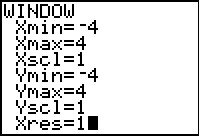
\includegraphics[width=2in]{./PolynomialsGraphics/RealZero01.jpg} \hspace{0.75in} & 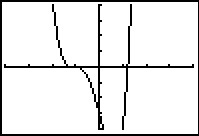
\includegraphics[width=2in]{./PolynomialsGraphics/RealZero02.jpg}

\end{tabular}
\end{center}

\item  In Example \ref{RZTex}, we learned that any rational zero of $f$ must be in the list $\left\{\pm \, \frac{1}{2}, \pm \, 1, \pm \, \frac{3}{2}, \pm \, 3\right\}$.  From the graph, it looks as if we can rule out any of the positive rational zeros, since the graph seems to cross the $x$-axis at a value just a little greater than $1$. On the negative side, $-1$ looks good, so we try that for our synthetic division.

\[\begin{array}{rrrrrr}

 -1 \, \, \vline& 2 & 4 & -1  & -6 & -3 \\

  & \downarrow     &  -2  &  -2  & 3 & 3\\ \hhline{~-----} 
  
  &  2            &   2  & -3 & -3 &  \fbox{$0$}  \\

\end{array}\]

We have a winner!  Remembering that $f$ was a fourth degree polynomial, we know that our quotient is a third degree polynomial.  If we can do one more successful division, we will have knocked the quotient down to a quadratic, and, if all else fails, we can use the quadratic formula to find the last two zeros.  Since there seems to be no other rational zeros to try, we continue with $-1$.  Also, the shape of the crossing at $x = -1$ leads us to wonder if the zero $x = -1$ has multiplicity 3.

\[\begin{array}{rrrrrr}
 -1 \, \, \vline& 2 & 4 & -1  & -6 & -3 \\

  & \downarrow     &  -2  &  -2  & 3 & 3\\ \hhline{~-----} 
  
  -1 \, \, \vline&  2 &   2  & -3 & -3 &  \fbox{$0$}  \\
    
               & \downarrow &  -2  &  0  & 3 &\\ \hhline{~----} 
 
   & 2  &   0  & -3& \fbox{0} &   \\
  
        

\end{array}\]


Success!  Our quotient polynomial is now $2x^2 - 3$.  Setting this to zero gives $2x^2 - 3 = 0$, or $x^2 = \frac{3}{2}$, which gives us $x = \pm \, \frac{\sqrt{6}}{2}$.  Concerning multiplicities, based on our division, we have that $-1$ has a multiplicity of at least $2$. The Factor Theorem tells us our remaining zeros, $\pm \, \frac{\sqrt{6}}{2}$, each have multiplicity at least $1$.  However, Theorem \ref{nzerosreal} tells us $f$ can have at most $4$ real zeros, counting multiplicity, and so we conclude that $-1$ is of multiplicity exactly $2$ and $\pm \, \frac{\sqrt{6}}{2}$ each has multiplicity $1$.  (Thus, we were \underline{wrong} to think that $-1$ had multiplicity $3$.) \qed

\end{enumerate}


\end{ex}

It is interesting to note that we could greatly improve on the graph of $y=f(x)$ in the previous example given to us by the calculator. For instance, from our determination of the zeros of $f$ and their multiplicities, we know the graph crosses at $x=-\frac{\sqrt{6}}{2} \approx -1.22$ then turns back upwards to touch the $x-$axis at $x=-1$. This tells us that, despite what the calculator showed us the first time, there is a relative maximum occurring at $x = -1$ and not a `flattened crossing' as we originally believed.  After resizing the window, we see not only the relative maximum but also a relative minimum\footnote{This is an example of what is called `hidden behavior.'} just to the left of $x = -1$ which shows us, once again, that Mathematics enhances the technology, instead of vice-versa.

\begin{center}

\begin{tabular}{cc}

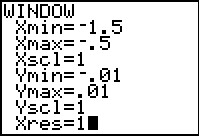
\includegraphics[width=2in]{./PolynomialsGraphics/RealZero03.jpg} \hspace{0.75in} & 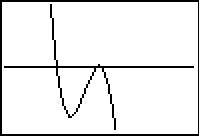
\includegraphics[width=2in]{./PolynomialsGraphics/RealZero04.jpg}

\end{tabular}
\end{center} 

Our next example shows how even a mild-mannered polynomial can cause problems.

\begin{ex}  Let $f(x) = x^4 + x^2 - 12$.

\begin{enumerate}

\item  Use Cauchy's Bound to determine an interval in which all of the real zeros of $f$ lie.

\item  Use the Rational Zeros Theorem to determine a list of possible rational zeros of $f$.

\item  Graph $y=f(x)$ using your graphing calculator.

\item  Find all of the real zeros of $f$ and their multiplicities.


\end{enumerate}

{\bf Solution.}

\begin{enumerate}

\item  Applying Cauchy's Bound, we find $M = 12$, so all of the real zeros lie in the interval $[-13,13]$.

\item  Applying the Rational Zeros Theorem with constant term $a_{\mbox{\tiny$0$}} = -12$ and leading coefficient $a_{\mbox{\tiny$4$}} = 1$, we get the list $\{\pm \, 1$, $\pm \, 2$, $\pm \, 3$, $\pm \, 4$, $\pm \, 6$, $\pm \, 12\}$.

\item  Graphing $y=f(x)$ on the interval $[-13,13]$ produces the graph below on the left.  Zooming in a bit gives the graph below on the right.  Based on the graph, none of our rational zeros will work. (Do you see why not?)


\begin{center}

\begin{tabular}{cc}

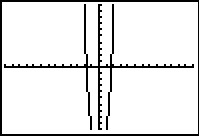
\includegraphics[width=2in]{./PolynomialsGraphics/RealZero05.jpg} \hspace{0.75in} & 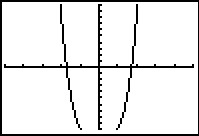
\includegraphics[width=2in]{./PolynomialsGraphics/RealZero06.jpg}

\end{tabular}
\end{center} 

\item  From the graph, we know $f$ has two real zeros, one positive, and one negative.  Our only hope at this point is to try and find the zeros of $f$ by setting $f(x)=x^4+x^2-12=0$ and solving.  If we stare at this equation long enough, we may recognize it as a `quadratic in disguise' or `quadratic in form'.   In other words, we have three terms: $x^4$, $x^2$ and $12$, and the exponent on the first term, $x^4$, is exactly twice that of the second term, $x^2$.  We may rewrite this as $\left(x^2\right)^2 + \left(x^2\right) - 12 = 0$.  To better see the forest for the trees, we momentarily replace $x^2$ with the variable $u$.  In terms of $u$, our equation becomes $u^2 + u - 12 = 0$, which we can readily factor as $(u+4)(u-3) = 0$.  In terms of $x$, this means $x^4+x^2-12= \left(x^2-3\right) \left(x^2 + 4 \right)=0$. We get $x^2 = 3$, which gives us $x = \pm \sqrt{3}$, or $x^2=-4$, which admits no real solutions.  Since $\sqrt{3} \approx 1.73$, the two zeros match what we expected from the graph.  In terms of multiplicity, the Factor Theorem guarantees $\left(x - \sqrt{3}\right)$ and $\left(x + \sqrt{3}\right)$ are factors of $f(x)$.  Since $f(x)$ can be factored as $f(x) = \left(x^2-3\right) \left(x^2 + 4 \right)$, and $x^2 + 4$ has no real zeros, the quantities $\left(x - \sqrt{3}\right)$ and $\left(x + \sqrt{3}\right)$ must both be factors of $x^2-3$.  According to Theorem \ref{nzerosreal}, $x^2-3$ can have at most $2$ zeros, counting multiplicity, hence each of $\pm \sqrt{3}$ is a zero of $f$ of multiplicity $1$. \qed

\end{enumerate}

\label{usubex}

\end{ex}

The technique used to factor $f(x)$ in Example \ref{usubex} is called \index{$u$-substitution} \textbf{{\boldmath $u$}-substitution}.  We shall see more of this technique in Section \ref{AlgebraicFunctions}.  In general, substitution can help us identify a `quadratic in disguise' provided that there are exactly three terms and the exponent of the first term is exactly twice that of the second.  It is entirely possible that a polynomial has no real roots at all, or worse, it has real roots but none of the techniques discussed in this section can help us find them exactly.  In the latter case, we are forced to approximate, which in this subsection means we use the `Zero' command on the graphing calculator.  


\subsection{For Those Wishing NOT to use a Graphing Calculator}

Suppose we wish to find the zeros of $f(x) = 2x^4+4x^3-x^2-6x-3$ \textit{without} using the calculator.  In this subsection, we present some more advanced mathematical tools (theorems) to help us.  Our first result is due to \href{http://en.wikipedia.org/wiki/Descartes}{\underline{Ren\'{e} Descartes}}.

\smallskip

\colorbox{ResultColor}{\bbm

\begin{thm} \index{Descartes' Rule of Signs}\label{DRS}  \textbf{Descartes' Rule of Signs:}  Suppose $f(x)$ is the formula for a polynomial function written with descending powers of $x$.

\begin{itemize}

\item If $P$ denotes the number of variations of sign in the formula for $f(x)$, then the number of positive real zeros (counting multiplicity) is one of the numbers \{$P$, $P-2$, $P-4$, \ldots \}.

\item If $N$ denotes the number of variations of sign in the formula for $f(-x)$, then the number of negative real zeros (counting multiplicity) is one of the numbers \{$N$, $N-2$, $N-4$, \dots\}.

\end{itemize}

\end{thm}
\ebm}

\smallskip

A few remarks are in order. First, to use Descartes' Rule of Signs, we need to understand what is meant by a \index{polynomial function ! variations in sign}\index{variations in sign}`\textbf{variation in sign}' of a polynomial function.  Consider $f(x) = 2x^4+4x^3-x^2-6x-3$.  If we focus on only the \textit{signs} of the coefficients, we start with a $(+)$, followed by another $(+)$, then switch to $(-)$, and stay $(-)$ for the remaining two coefficients.  Since the signs of the coefficients switched \textit{once} as we read from left to right, we say that $f(x)$ has \textit{one} variation in sign.  When we speak of the variations in sign of a polynomial function $f$ we assume the formula for $f(x)$ is written with descending powers of $x$, as in Definition \ref{polynomialfunction}, and concern ourselves only with the nonzero coefficients.  Second, unlike the Rational Zeros Theorem, Descartes' Rule of Signs gives us an estimate to the \textit{number} of positive and negative real zeros, not the actual \textit{value} of the zeros. Lastly, Descartes' Rule of Signs counts multiplicities.  This means that, for example, if one of the zeros has multiplicity $2$, Descsartes' Rule of Signs would count this as \textit{two} zeros.  Lastly, note that the number of positive or negative real zeros always starts with the number of sign changes and decreases by an even number.  For example, if $f(x)$ has $7$ sign changes, then, counting multplicities, $f$ has either $7$, $5$, $3$ or $1$ positive real zero.  This implies that the graph of $y=f(x)$ crosses the positive $x$-axis at least once.  If $f(-x)$ results in $4$ sign changes, then, counting multiplicities, $f$ has $4$, $2$ or $0$ negative real zeros;  hence, the graph of $y=f(x)$ may not cross the negative $x$-axis at all.  The proof of Descartes' Rule of Signs is a bit technical, and can be found \href{http://www.cut-the-knot.org/fta/ROS2.shtml}{\underline{here}}. 

\begin{ex}  Let $f(x) = 2x^4+4x^3-x^2-6x-3$.  Use Descartes' Rule of Signs to determine the possible number and location of the real zeros of $f$.

\smallskip

{\bf Solution.}  As noted above, the variations of sign of $f(x)$ is $1$. This means, counting multiplicities, $f$ has exactly $1$ positive real zero.  Since $f(-x)=2(-x)^4+4(-x)^3-(-x)^2-6(-x)-3=2x^4-4x^3-x^2+6x-3$ has $3$ variations in sign, $f$ has either $3$ negative real zeros or $1$ negative real zero, counting multiplicities. \qed

\label{DRSex}

\end{ex}

Cauchy's Bound gives us a general bound on the zeros of a polynomial function.  Our next result helps us determine bounds on the real zeros of a polynomial as we synthetically divide which are often sharper\footnote{That is, better, or more accurate.} bounds than Cauchy's Bound.   

\smallskip

\colorbox{ResultColor}{\bbm
\begin{thm}  \label{ULbounds} \textbf{Upper and Lower Bounds:}  Suppose $f$ is a polynomial of degree $n \geq 1$. \index{Upper and Lower Bounds Theorem}\index{polynomial function ! zero ! upper bound}\index{polynomial function ! zero ! lower bound}\index{zero ! upper and lower bounds}

\begin{itemize}

\item  If $c > 0$ is synthetically divided into $f$ and all of the numbers in the final line of the division tableau have the same signs, then $c$ is an upper bound for the real zeros of $f$.  That is, there are no real zeros greater than $c$.

\item  If $c < 0$ is synthetically divided into $f$ and the numbers in the final line of the division tableau alternate signs, then $c$ is a lower bound for the real zeros of $f$.  That is, there are no real zeros less than $c$.

\textbf{NOTE:}  If the number $0$ occurs in the final line of the division tableau in either of the above cases, it can be treated as $(+)$ or $(-)$ as needed.

\end{itemize}

\end{thm}
\ebm}


\smallskip

The Upper and Lower Bounds Theorem works because of Theorem \ref{polydiv}.  For the upper bound part of the theorem, suppose $c>0$ is divided into $f$ and the resulting line in the division tableau contains, for example, all nonnegative numbers.  This means $f(x) = (x-c) q(x) + r$, where the coefficients of the quotient polynomial and the remainder are nonnegative.  (Note that the leading coefficient of $q$ is the same as $f$ so $q(x)$ is not the zero polynomial.)  If $b > c$, then $f(b) = (b-c) q(b) + r$, where $(b-c)$ and  $q(b)$ are both positive and $r \geq 0$.  Hence $f(b) > 0$ which shows $b$ cannot be a zero of $f$.  Thus no real number $b > c$ can be a zero of $f$, as required.  A similar argument proves $f(b) < 0$ if all of the numbers in the final line of the synthetic division tableau are non-positive.  To prove the lower bound part of the theorem, we note that a lower bound for the negative real zeros of $f(x)$ is an upper bound for the positive real zeros of $f(-x)$.  Applying the upper bound portion to $f(-x)$ gives the result.  (Do you see where the alternating signs come in?) With the additional mathematical machinery of Descartes' Rule of Signs and the Upper and Lower Bounds Theorem, we can find the real zeros of $f(x) = 2x^4+4x^3-x^2-6x-3$ without the use of a graphing calculator.

\begin{ex}  Let $f(x) = 2x^4+4x^3-x^2-6x-3$.

\begin{enumerate}

\item  Find all of the real zeros of $f$ and their multiplicities.

\item Sketch the graph of $y=f(x)$.

\end{enumerate}  

{\bf Solution.}  \begin{enumerate}

\item  We know from Cauchy's Bound that all of the real zeros lie in the interval $[-4,4]$ and that our possible rational zeros are $\pm \, \frac{1}{2}$, $\pm \, 1$, $\pm \, \frac{3}{2}$ and $\pm \, 3$.  Descartes' Rule of Signs guarantees us at least one negative real zero and exactly one positive real zero, counting multiplicity.  We try our positive rational zeros, starting with the smallest, $\frac{1}{2}$.  Since the remainder isn't zero, we know $\frac{1}{2}$ isn't a zero.  Sadly, the final line in the division tableau has both positive and negative numbers, so $\frac{1}{2}$ is not an upper bound.  The only information we get from this division is courtesy of the Remainder Theorem which tells us $f\left(\frac{1}{2}\right) =  -\frac{45}{8}$ so the point $\left(\frac{1}{2}, -\frac{45}{8}\right)$ is on the graph of $f$.  We continue to our next possible zero, $1$.  As before, the only information we can glean from this is that $(1,-4)$ is on the graph of $f$.  When we try our next possible zero, $\frac{3}{2}$, we get that it is not a zero, and we also see that it is an upper bound on the zeros of $f$, since all of the numbers in the final line of the division tableau are positive.  This means there is no point trying our last possible rational zero, $3$.  Descartes' Rule of Signs guaranteed us a positive real zero, and at this point we have shown this zero is irrational.  Furthermore, the Intermediate Value Theorem, Theorem \ref{IVT}, tells us the zero lies between $1$ and $\frac{3}{2}$, since $f(1) < 0$ and $f\left(\frac{3}{2}\right) > 0$.   \smallskip

\begin{tabular}{ccc}

$\begin{array}{rrrrrr}

 \frac{1}{2} \, \, \vline& 2 & 4 & -1  & -6 & -3 \\

  & \downarrow     &  1  &  \frac{5}{2}  & \frac{3}{4} & -\frac{21}{8} \\ [4pt] \hhline{~-----}
  
  &  2            &   5  &  \frac{3}{2} & -\frac{21}{4} &  \fbox{$-\frac{45}{8}$}  \\

\end{array}$ &     

$\begin{array}{rrrrrr}

1 \, \, \vline& 2 & 4 & -1  & -6 & -3 \\

  & \downarrow     &  2 &  6  & 5 & -1 \\ [4pt] \hhline{~-----}
  
  &  2            &   6  &  5 & -1 &  \fbox{$-4$}  \\

\end{array}$  &

             
$\begin{array}{rrrrrr}

\frac{3}{2} \, \, \vline& 2 & 4 & -1  & -6 & -3 \\

  & \downarrow     &  3 &  \frac{21}{2}  & \frac{57}{4} & \frac{99}{8} \\ [4pt] \hhline{~-----}
  
  &  2            &   7  &  \frac{19}{2} & \frac{33}{4} &  \fbox{$\frac{75}{8}$}  \\

\end{array}$

\end{tabular}

\smallskip

We now turn our attention to negative real zeros.  We try the largest possible zero, $-\frac{1}{2}$.  Synthetic division shows us it is not a zero, nor is it a lower bound (since the numbers in the final line of the division tableau do not alternate), so we proceed to $-1$.  This division shows $-1$ is a zero.  Descartes' Rule of Signs told us that we may have up to three negative real zeros, counting multiplicity, so we try $-1$ again, and it works once more.  At this point, we have taken $f$, a fourth degree polynomial, and performed two successful divisions.  Our quotient polynomial is quadratic, so we look at it to find the remaining zeros.

\begin{tabular}{cc}

$\begin{array}{rrrrrr}

 -\frac{1}{2} \, \, \vline& 2 & 4 & -1  & -6 & -3 \\

  & \downarrow     &  -1  &  -\frac{3}{2}  & \frac{5}{4} & \frac{19}{8} \\ [4pt] \hhline{~-----}
  
  &  2            &   3  &  -\frac{5}{2} & -\frac{19}{4} &  \fbox{$-\frac{5}{8}$}  \\

\end{array}$ &  \hspace{1in}

$\begin{array}{rrrrrr}
 -1 \, \, \vline& 2 & 4 & -1  & -6 & -3 \\

  & \downarrow     &  -2  &  -2  & 3 & 3\\ \hhline{~-----} 
  
  -1 \, \, \vline&  2 &   2  & -3 & -3 &  \fbox{$0$}  \\
    
               & \downarrow &  -2  &  0  & 3 &\\ \hhline{~----} 
 
   & 2  &   0  & -3& \fbox{0} &   \\
  
        

\end{array}$  

\end{tabular}

\smallskip

Setting the quotient polynomial equal to zero yields $2x^2 - 3 = 0$, so that $x^2 = \frac{3}{2}$, or $x = \pm \, \frac{\sqrt{6}}{2}$.  Descartes' Rule of Signs tells us that the positive real zero we found, $\frac{\sqrt{6}}{2}$, has multiplicity $1$.  Descartes also tells us the total multiplicity of negative real zeros is $3$, which forces $-1$ to be a zero of multiplicity $2$ and $- \frac{\sqrt{6}}{2}$ to have multiplicity $1$.  

\item  We know the end behavior of $y=f(x)$ resembles that of its leading term $y=2x^4$.  This means that the graph enters the scene in Quadrant II and exits in Quadrant I.  Since $\pm \, \frac{\sqrt{6}}{2}$ are zeros of odd multiplicity, we have that the graph crosses through the $x$-axis at the points $\left( -\frac{\sqrt{6}}{2}, 0 \right)$ and $\left( \frac{\sqrt{6}}{2}, 0 \right)$.  Since $-1$ is a zero of multiplicity $2$, the graph of $y=f(x)$ touches and rebounds off the $x$-axis at $(-1,0)$.  Putting this together, we get

\begin{center}

\begin{mfpic}[15]{-4}{4}{-6}{6}
\axes
\tlabel[cc](4,-0.5){\scriptsize $x$}
\tlabel[cc](0.5,6){\scriptsize $y$}
\arrow \reverse \arrow \function{-3.5,3.25,0.1}{0.1*(x+3)*((x+1)**2)*(x-3)}
\point[3pt]{(-3,0),(-1,0),(3,0)}
\end{mfpic}

\end{center}

\qed

\end{enumerate}

\end{ex}

You can see why the `no calculator' approach is not very popular these days.  It requires more computation and more theorems than the alternative.\footnote{This is apparently a bad thing.}  In general, no matter how many theorems you throw at a polynomial, it may well be impossible\footnote{We don't use this word lightly;  it can be proven that the zeros of some polynomials cannot be expressed using the usual algebraic symbols.} to find their zeros exactly.  The polynomial $f(x) = x^5-x-1$ is one such beast.\footnote{See this \href{http://en.wikipedia.org/wiki/Galois_theory}{\underline{page}}.}  According to Descartes' Rule of Signs, $f$ has exactly one positive real zero, and it could have two negative real zeros, or none at all.  The Rational Zeros Test gives us $\pm 1$ as rational zeros to try but neither of these work since $f(1) = f(-1) = -1$.  If we try the substitution technique we used in Example \ref{usubex}, we find $f(x)$ has three terms, but the exponent on the $x^5$ isn't exactly twice the exponent on $x$.  How could we go about approximating the positive zero without resorting to the `Zero' command of a graphing calculator?  We use the \index{Bisection Method} \textbf{Bisection Method}.  The first step in the Bisection Method is to find an interval on which $f$ changes sign.  We know $f(1) = -1$ and we find $f(2) = 29$.  By the Intermediate Value Theorem, we know that the zero of $f$ lies in the interval $[1,2]$.  Next, we `bisect' this interval and find the midpoint is $1.5$.  We have that $f(1.5)\approx 5.09$.  This means that our zero is between $1$ and $1.5$, since $f$ changes sign on this interval.  Now, we `bisect' the interval $[1,1.5]$ and find $f(1.25) \approx 0.80$, so now we have the zero between $1$ and $1.25$.  Bisecting $[1,1.25]$, we find $f(1.125) \approx -0.32$, which means the zero of $f$ is between $1.125$ and $1.25$.  We continue in this fashion until we have `sandwiched' the zero between two numbers which differ by no more than a desired accuracy. You can think of the Bisection Method as reversing the sign diagram process:  instead of finding the zeros and checking the sign of $f$ using test values, we are using test values to determine where the signs switch to find the zeros.  It is a slow and tedious, yet fool-proof, method for approximating a real zero.  

\medskip

Our next example reminds us of the role finding zeros plays in solving equations and inequalities.

\begin{ex}  \label{polyeqineqexample} $~$

\begin{enumerate}

\item  Find all of the real solutions to the equation $2x^5+6x^3+3 = 3x^4+8x^2$. 

\item  Solve the inequality $2x^5+6x^3+3 \leq 3x^4+8x^2$.

\item  Interpret your answer to part 2 graphically, and verify using a graphing calculator.


\end{enumerate}

{\bf Solution.} 

\begin{enumerate}

\item  Finding the real solutions to $2x^5+6x^3+3 = 3x^4+8x^2$ is the same as finding the real solutions to $2x^5-3x^4+6x^3-8x^2+3=0$.  In other words, we are looking for the real zeros of $p(x)=  2x^5-3x^4+6x^3-8x^2+3$.  Using the techniques developed in this section, we get

\[\begin{array}{rrrrrrr}
1 \, \, \vline& 2 & -3 & 6  & -8 & 0 &3 \\

  & \downarrow     &  2  &  -1  & 5 & -3 & -3\\ \hhline{~------} 

 1 \, \, \vline& 2 & -1 & 5  & -3 & -3 & \fbox{$0$} \\

  & \downarrow     &  2 &  1  & 6 & 3 &\\ \hhline{~-----} 
  
  -\frac{1}{2} \, \, \vline&  2 &  1  & 6 & 3 &  \fbox{$0$} & \\
    
               & \downarrow &  -1  &  0  & -3 &&\\ \hhline{~----} 
 
   & 2  &   0  & 6& \fbox{0} &&   \\
  


\end{array}\]


The quotient polynomial is $2x^2 + 6$ which has no real zeros so we get $x=-\frac{1}{2}$ and $x=1$.   

\item To solve this nonlinear inequality, we follow the same guidelines set forth in Section \ref{Inequalities}:  we get $0$ on one side of the inequality and construct a sign diagram.  Our original inequality can be rewritten as $2x^5-3x^4+6x^3-8x^2+3 \leq 0$.  We found the zeros of $p(x) = 2x^5-3x^4+6x^3-8x^2+3$ in part 1 to be $x=-\frac{1}{2}$ and $x=1$. We construct our sign diagram as before.

\begin{center}

\begin{mfpic}[10]{-5}{5}{-2}{2}
\arrow \reverse \arrow \polyline{(-5,0),(5,0)}
\xmarks{-2,2}
\arrow \polyline{(-3.5,-1.5),(-3.5,-0.5)}
\arrow \polyline{(0,-1.5),(0,-0.5)}
\arrow \polyline{(3.5,-1.5),(3.5,-0.5)}
\tlpointsep{4pt}
\axislabels {x}{{$-\frac{1}{2} \hspace{7pt}$} -2, {$1$} 2}
\tlabel[cc](-3.5,1){$(-)$}
\tlabel[cc](-2,1){$0$}
\tlabel[cc](0,1){$(+)$}
\tlabel[cc](2,1){$0$}
\tlabel[cc](3.5,1){$(+)$}
\tlabel[cc](-3.5,-2.25){$-1$}
\tlabel[cc](0,-2.25){$0$}
\tlabel[cc](3.5,-2.25){$2$}
\end{mfpic} 

\end{center}

The solution to $p(x) < 0$ is $\left(-\infty, -\frac{1}{2}\right)$, and we know $p(x) = 0$ at $x=-\frac{1}{2}$ and $x=1$.  Hence, the solution to $p(x) \leq 0$ is $\left(-\infty, -\frac{1}{2}\right] \cup \left\{1\right\}$.  


\item To interpret this solution graphically, we set $f(x) = 2x^5+6x^3+3$ and $g(x) = 3x^4+8x^2$.  We recall that the solution to $f(x) \leq g(x)$ is the set of $x$ values for which the graph of $f$ is below the graph of $g$ (where $f(x) < g(x)$) along with the $x$ values where the two graphs intersect ($f(x) = g(x)$).  Graphing $f$ and $g$ on the calculator produces the picture on the lower left.  (The end behavior should tell you which is which.)  We see that the graph of $f$ is below the graph of $g$ on $\left(-\infty, -\frac{1}{2}\right)$. However, it is difficult to see what is happening near $x=1$.  Zooming in (and making the graph of $g$ thicker), we see that the graphs of $f$ and $g$ do intersect at $x=1$, but the graph of $g$ remains below the graph of $f$ on either side of $x = 1$.

\begin{center}

\begin{tabular}{cc}

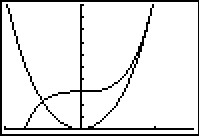
\includegraphics[width=2in]{./PolynomialsGraphics/RealZero07.jpg} \hspace{0.75in} & 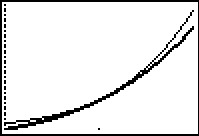
\includegraphics[width=2in]{./PolynomialsGraphics/RealZero08.jpg}

\end{tabular}
\end{center} 

\qed
\end{enumerate}

\end{ex}

Our last example revisits an application from page \pageref{LCDmaxprofit} in the Exercises of Section \ref{GraphsofPolynomials}.

\begin{ex} Suppose the profit $P$, in \textit{thousands} of dollars, from producing and selling $x$ \textit{hundred} LCD TVs is given by  $P(x)=-5x^3+35x^2-45x-25$, $0 \leq x \leq 10.07$.  How many TVs should be produced to make a profit?  Check your answer using a graphing utility.

\smallskip

{\bf Solution.}  To `make a profit' means to solve $P(x) = -5x^3+35x^2-45x-25 > 0$, which we do analytically using a sign diagram.  To simplify things, we first factor out the $-5$ common to all the coefficients to get $-5\left(x^3 - 7x^2+9x-5\right) > 0$, so we can just focus on finding the zeros of $f(x) = x^3-7x^2+9x+5$.  The possible rational zeros of $f$ are $\pm 1$ and $\pm 5$, and going through the usual computations, we find $x=5$ is the only rational zero.  Using this, we factor $f(x) = x^3-7x^2+9x+5 = (x-5) \left(x^2-2x-1\right)$, and we find the remaining zeros by applying the Quadratic Formula to $x^2-2x-1 = 0$.  We find three real zeros,  $x=1-\sqrt{2} = -0.414 \ldots$,  $x = 1+\sqrt{2} = 2.414 \ldots$, and $x = 5$, of which only the last two fall in the applied domain of $[0, 10.07]$.  We choose $x=0$, $x=3$ and $x=10.07$ as our test values and plug them into the function $P(x)=-5x^3+35x^2-45x-25$ (not $f(x) =x^3 - 7x^2+9x-5$) to get the sign diagram below.

\begin{center}

\begin{mfpic}[10]{-5}{5}{-2}{2}
\polyline{(-5,0),(5,0)}
\point[3pt]{(-5,0), (5,0)}
\xmarks{-2,2}
\arrow \polyline{(-5,-1.5),(-5,-0.5)}
\arrow \polyline{(0,-1.5),(0,-0.5)}
\arrow \polyline{(5,-1.5),(5,-0.5)}
\tlpointsep{4pt}
\axislabels {x}{{\scriptsize $1+\sqrt{2} \hspace{7pt}$} -2, {\scriptsize $5$} 2}
\tlabel[cc](-5,1){$(-)$}
\tlabel[cc](-2,1){$0$}
\tlabel[cc](0,1){$(+)$}
\tlabel[cc](2,1){$0$}
\tlabel[cc](-5,-2.25){$0$}
\tlabel[cc](0,-2.25){$3$}
\tlabel[cc](5,-2.25){$10.07$}
\tlabel[cc](5,1){$(-)$}
\end{mfpic} 

\end{center}

We see immediately that $P(x)>0$ on $(1+\sqrt{2},5)$.  Since $x$ measures the number of TVs in \textit{hundreds}, $x = 1 + \sqrt{2}$ corresponds to $241.4\ldots$ TVs.  Since we can't produce a fractional part of a TV, we need to choose between producing 241 and 242 TVs.  From the sign diagram, we see that $P(2.41) < 0$ but $P(2.42)>0$ so, in this case we take the next \textit{larger} integer value and set the minimum production to 242 TVs.  At the other end of the interval, we have $x=5$ which corresponds to $500$ TVs.  Here, we take the next \textit{smaller} integer value, $499$ TVs to ensure that we make a profit.  Hence, in order to make a profit, at least 242, but no more than 499 TVs need to be produced.  To check our answer using a calculator, we graph $y=P(x)$ and make use of the `Zero' command. We see that the calculator approximations bear out our analysis.\footnote{Note that the $y$-coordinates of the points here aren't registered as $0$.  They are expressed in Scientific Notation.  For instance, $1 \mbox{\tiny $E$} -11$ corresponds to $0.00000000001$, which is pretty close in the calculator's eyes\footnotemark to $0$.} \footnotetext{but not a Mathematician's}  

\begin{center}

\begin{tabular}{cc}

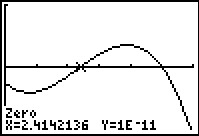
\includegraphics[width=2in]{./PolynomialsGraphics/LCDIneqZero1.jpg} \hspace{0.75in} & 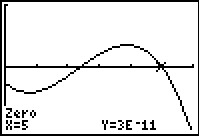
\includegraphics[width=2in]{./PolynomialsGraphics/LCDIneqZero2.jpg}

\end{tabular}

\end{center}   \qed

\end{ex}

\newpage

\subsection{Exercises}


In Exercises \ref{prelimpolystufffirst} - \ref{prelimpolystufflast}, for the given polynomial:

\begin{itemize}
\item  Use Cauchy's Bound to find an interval containing all of the real zeros.
\item  Use the Rational Zeros Theorem to make a list of possible rational zeros.
\item  Use Descartes' Rule of Signs to list the possible number of positive and negative real zeros, counting multiplicities.
\end{itemize}


\begin{multicols}{2}
\begin{enumerate}

\item $f(x) = x^{3} - 2x^{2} - 5x + 6$ \label{prelimpolystufffirst}
\item $f(x) = x^{4} + 2x^{3} - 12x^{2} - 40x - 32$

\setcounter{HW}{\value{enumi}}
\end{enumerate}
\end{multicols}

\begin{multicols}{2}
\begin{enumerate}
\setcounter{enumi}{\value{HW}}

\item $f(x) = x^{4} - 9x^{2} - 4x + 12$
\item $f(x) = x^{3} + 4x^{2} - 11x + 6$

\setcounter{HW}{\value{enumi}}
\end{enumerate}
\end{multicols}

\begin{multicols}{2}
\begin{enumerate}
\setcounter{enumi}{\value{HW}}

\item $f(x) = x^{3} - 7x^{2} + x - 7$
\item $f(x) = -2x^{3} + 19x^{2} - 49x + 20$

\setcounter{HW}{\value{enumi}}
\end{enumerate}
\end{multicols}

\begin{multicols}{2}
\begin{enumerate}
\setcounter{enumi}{\value{HW}}

\item $f(x) = -17x^{3} + 5x^{2} + 34x - 10$
\item $f(x) = 36x^{4} - 12x^{3} - 11x^{2} + 2x + 1$

\setcounter{HW}{\value{enumi}}
\end{enumerate}
\end{multicols}

\begin{multicols}{2}
\begin{enumerate}
\setcounter{enumi}{\value{HW}}

\item $f(x) = 3x^{3} + 3x^{2} - 11x - 10$
\item $f(x) = 2x^4+x^3-7x^2-3x+3$ \label{prelimpolystufflast}


\setcounter{HW}{\value{enumi}}
\end{enumerate}
\end{multicols}


In Exercises \ref{findrealzerosexerfirst} - \ref{findrealzerosexerlast}, find the real zeros of the polynomial using the techniques specified by your instructor.  State the multiplicity of each real zero.


\begin{multicols}{2}
\begin{enumerate}
\setcounter{enumi}{\value{HW}}

\item $f(x) = x^{3} - 2x^{2} - 5x + 6$ \label{findrealzerosexerfirst}
\item $f(x) = x^{4} + 2x^{3} - 12x^{2} - 40x - 32$

\setcounter{HW}{\value{enumi}}
\end{enumerate}
\end{multicols}

\begin{multicols}{2}
\begin{enumerate}
\setcounter{enumi}{\value{HW}}

\item $f(x) = x^{4} - 9x^{2} - 4x + 12$
\item $f(x) = x^{3} + 4x^{2} - 11x + 6$

\setcounter{HW}{\value{enumi}}
\end{enumerate}
\end{multicols}

\begin{multicols}{2}
\begin{enumerate}
\setcounter{enumi}{\value{HW}}

\item $f(x) = x^{3} - 7x^{2} + x - 7$
\item $f(x) = -2x^{3} + 19x^{2} - 49x + 20$

\setcounter{HW}{\value{enumi}}
\end{enumerate}
\end{multicols}

\begin{multicols}{2}
\begin{enumerate}
\setcounter{enumi}{\value{HW}}

\item $f(x) = -17x^{3} + 5x^{2} + 34x - 10$
\item $f(x) = 36x^{4} - 12x^{3} - 11x^{2} + 2x + 1$

\setcounter{HW}{\value{enumi}}
\end{enumerate}
\end{multicols}

\begin{multicols}{2}
\begin{enumerate}
\setcounter{enumi}{\value{HW}}

\item $f(x) = 3x^{3} + 3x^{2} - 11x - 10$
\item $f(x) = 2x^4+x^3-7x^2-3x+3$

\setcounter{HW}{\value{enumi}}
\end{enumerate}
\end{multicols}

\begin{multicols}{2}
\begin{enumerate}
\setcounter{enumi}{\value{HW}}

\item $f(x) = 9x^{3} - 5x^{2} - x$
\item $f(x) = 6x^{4} - 5x^{3} - 9x^{2}$

\setcounter{HW}{\value{enumi}}
\end{enumerate}
\end{multicols}

\begin{multicols}{2}
\begin{enumerate}
\setcounter{enumi}{\value{HW}}

\item $f(x) = x^4+2x^2 - 15$
\item $f(x) = x^4-9x^2+14$

\setcounter{HW}{\value{enumi}}
\end{enumerate}
\end{multicols}

\begin{multicols}{2}
\begin{enumerate}
\setcounter{enumi}{\value{HW}}

\item $f(x) = 3x^4-14x^2-5$
\item $f(x) = 2x^4-7x^2+6$

\setcounter{HW}{\value{enumi}}
\end{enumerate}
\end{multicols}

\begin{multicols}{2}
\begin{enumerate}
\setcounter{enumi}{\value{HW}}

\item $f(x) = x^6-3x^3-10$
\item $f(x) = 2x^6-9x^3+10$

\setcounter{HW}{\value{enumi}}
\end{enumerate}
\end{multicols}

\begin{multicols}{2}
\begin{enumerate}
\setcounter{enumi}{\value{HW}}

\item $f(x) = x^5-2x^4-4x+8$
\item $f(x) = 2x^5+3x^4-18x-27$ \label{findrealzerosexerlast}

\setcounter{HW}{\value{enumi}}
\end{enumerate}
\end{multicols}

\pagebreak

In Exercises \ref{realzeroswcalcfirst} - \ref{realzeroswcalclast}, use your calculator,\footnote{You \textit{can} do these without your calculator, but it may test your mettle!} to help you find the real zeros of the polynomial.  State the multiplicity of each real zero.

\begin{enumerate}
\setcounter{enumi}{\value{HW}}

\item $f(x) = x^{5} - 60x^{3} - 80x^{2} + 960x + 2304$ \label{realzeroswcalcfirst}
\item $f(x) = 25x^{5} - 105x^{4} + 174x^{3} - 142x^{2} + 57x - 9$
\item $f(x) = 90x^{4} - 399x^{3} + 622x^{2} - 399x + 90$ \label{realzeroswcalclast}

\setcounter{HW}{\value{enumi}}
\end{enumerate}

\begin{enumerate}
\setcounter{enumi}{\value{HW}}

\item Find the real zeros of $f(x) = x^{3} - \frac{1}{12}x^{2} - \frac{7}{72}x + \frac{1}{72}$ by first finding a polynomial $q(x)$ with integer coefficients such that $q(x) = N \cdot f(x)$ for some integer $N$.  (Recall that the Rational Zeros Theorem required the polynomial in question to have integer coefficients.) Show that $f$ and $q$ have the same real zeros.

\setcounter{HW}{\value{enumi}}
\end{enumerate}

In Exercises \ref{polyequexerfirst} - \ref{polyequexerlast}, find the real solutions of the polynomial equation.  (See Example \ref{polyeqineqexample}.)

\begin{multicols}{2}
\begin{enumerate}
\setcounter{enumi}{\value{HW}}

\item  $9x^{3} = 5x^{2} + x$  \label{polyequexerfirst} 
\item $9x^{2}+5x^{3}= 6x^{4}$  

\setcounter{HW}{\value{enumi}}
\end{enumerate}
\end{multicols}

\begin{multicols}{2}
\begin{enumerate}
\setcounter{enumi}{\value{HW}}

\item $x^{3} + 6 = 2x^{2} + 5x$ 
\item $x^{4} + 2x^{3} = 12x^{2} + 40x + 32$ 

\setcounter{HW}{\value{enumi}}
\end{enumerate}
\end{multicols}


\begin{multicols}{2}
\begin{enumerate}
\setcounter{enumi}{\value{HW}}

\item $x^{3} - 7x^{2} = 7-x$ 
\item $2x^{3} = 19x^{2} - 49x + 20$ 

\setcounter{HW}{\value{enumi}}
\end{enumerate}
\end{multicols}

\begin{multicols}{2}
\begin{enumerate}
\setcounter{enumi}{\value{HW}}

\item $x^{3} + x^{2} = \dfrac{11x + 10}{3}$ 
\item $x^4+2x^2 = 15$ 


\setcounter{HW}{\value{enumi}}
\end{enumerate}
\end{multicols}

\begin{multicols}{2}
\begin{enumerate}
\setcounter{enumi}{\value{HW}}

\item $14x^{2}+5=3x^{4}$  

\item $2x^5+3x^4 = 18x + 27$ \label{polyequexerlast}  

\setcounter{HW}{\value{enumi}}
\end{enumerate}
\end{multicols}


In Exercises \ref{polyinequexerfirst} - \ref{polyinequexerlast}, solve the polynomial inequality and state your answer using interval notation.



\begin{multicols}{2}
\begin{enumerate}
\setcounter{enumi}{\value{HW}}

\item $-2x^{3} + 19x^{2} - 49x + 20 > 0$ \label{polyinequexerfirst}
\item $x^{4} - 9x^{2} \leq 4x - 12$

\setcounter{HW}{\value{enumi}}
\end{enumerate}
\end{multicols}

\begin{multicols}{2}
\begin{enumerate}
\setcounter{enumi}{\value{HW}}

\item $(x - 1)^{2} \geq 4$
\item $4x^3 \geq 3x+1$

\setcounter{HW}{\value{enumi}}
\end{enumerate}
\end{multicols}

\begin{multicols}{2}
\begin{enumerate}
\setcounter{enumi}{\value{HW}}

\item $x^4 \leq 16+4x-x^3$
\item $3x^2 + 2x < x^4$

\setcounter{HW}{\value{enumi}}
\end{enumerate}
\end{multicols}

\begin{multicols}{2}
\begin{enumerate}
\setcounter{enumi}{\value{HW}}

\item $\dfrac{x^3+2 x^2}{2} < x+2$
\item $\dfrac{x^3+20x}{8} \geq x^2 + 2$

\setcounter{HW}{\value{enumi}}
\end{enumerate}
\end{multicols}

\begin{multicols}{2}
\begin{enumerate}
\setcounter{enumi}{\value{HW}}

\item $2x^4>5x^2+3$
\item $x^6 + x^3 \geq 6$ \label{polyinequexerlast}

\setcounter{HW}{\value{enumi}}
\end{enumerate}
\end{multicols}

\begin{enumerate}
\setcounter{enumi}{\value{HW}}

\item  In Example \ref{boxnotopex} in Section \ref{GraphsofPolynomials}, a box with no top is constructed from a $10$ inch $\times$ $12$ inch piece of cardboard by cutting out congruent squares from each corner of the cardboard and then folding the resulting tabs.  We determined the volume of that box (in cubic inches) is given by  $V(x) = 4x^3-44x^2+120x$, where $x$ denotes the length of the side of the square which is removed from each corner (in inches), $0 < x < 5$.  Solve the inequality $V(x) \geq 80$ analytically and interpret your answer in the context of that example.

\item  From Exercise \ref{newportaboycost} in Section \ref{GraphsofPolynomials}, $C(x) = .03x^{3} - 4.5x^{2} + 225x + 250$, for $x \geq 0$ models the cost, in dollars, to produce $x$ PortaBoy game systems. If the production budget is $\$5000$, find the number of game systems which can be produced and still remain under budget.

\item Let $f(x) = 5x^{7} - 33x^{6} + 3x^{5} - 71x^{4} - 597x^{3} + 2097x^{2} - 1971x + 567$.  With the help of your classmates, find the $x$- and $y$- intercepts of the graph of $f$.  Find the intervals on which the function is increasing, the intervals on which it is decreasing and the local extrema.  Sketch the graph of $f$, using more than one picture if necessary to show all of the important features of the graph.  

\item With the help of your classmates, create a list of five polynomials with different degrees whose real zeros cannot be found using any of the techniques in this section.

\setcounter{HW}{\value{enumi}}
\end{enumerate}
 



\newpage

\subsection{Answers}

\begin{enumerate}

\item For $f(x) = x^{3} - 2x^{2} - 5x + 6$
\begin{itemize}
\item  All of the real zeros lie in the interval $[-7,7]$
\item  Possible rational zeros are $\pm 1$, $\pm 2$, $\pm 3$, $\pm 6$
\item  There are 2 or 0 positive real zeros;  there is 1 negative real zero
\end{itemize}

\item For  $f(x) = x^{4} + 2x^{3} - 12x^{2} - 40x - 32$
\begin{itemize}
\item  All of the real zeros lie in the interval $[-41,41]$
\item  Possible rational zeros are $\pm 1$, $\pm 2$, $\pm 4$, $\pm 8$, $\pm 16$, $\pm 32$
\item  There is 1 positive real zero;  there are 3 or 1 negative real zeros
\end{itemize}

\item For  $f(x) = x^{4} - 9x^{2} - 4x + 12$
\begin{itemize}
\item  All of the real zeros lie in the interval $[-13,13]$
\item  Possible rational zeros are $\pm 1$, $\pm 2$, $\pm 3$, $\pm 4$, $\pm 6$, $\pm 12$
\item  There are 2 or 0 positive real zeros;  there are 2 or 0 negative real zeros
\end{itemize}

\item For  $f(x) = x^{3} + 4x^{2} - 11x + 6$
\begin{itemize}
\item  All of the real zeros lie in the interval $[-12,12]$
\item  Possible rational zeros are $\pm 1$, $\pm 2$, $\pm 3$, $\pm 6$
\item  There are 2 or 0 positive real zeros;  there is 1 negative real zero
\end{itemize}

\item For   $f(x) = x^{3} - 7x^{2} + x - 7$
\begin{itemize}
\item  All of the real zeros lie in the interval $[-8,8]$
\item  Possible rational zeros are $\pm 1$, $\pm 7$
\item  There are 3 or 1 positive real zeros;  there are no negative real zeros
\end{itemize}

\item For   $f(x) = -2x^{3} + 19x^{2} - 49x + 20$
\begin{itemize}
\item  All of the real zeros lie in the interval $\left[-\frac{51}{2},\frac{51}{2} \right]$
\item  Possible rational zeros are  $\pm \frac{1}{2}$, $\pm 1$, $\pm 2$, $\pm \frac{5}{2}$, $\pm 4$, $\pm 5$, $\pm 10$, $\pm 20$ 
\item  There are 3 or 1 positive real zeros;  there are no negative real zeros
\end{itemize}

\item For   $f(x) = -17x^{3} + 5x^{2} + 34x - 10$
\begin{itemize}
\item  All of the real zeros lie in the interval $[-3,3]$
\item  Possible rational zeros are $\pm \frac{1}{17}$, $\pm \frac{2}{17}$, $\pm \frac{5}{17}$, $\pm \frac{10}{17}$, $\pm 1$, $\pm 2$, $\pm 5$, $\pm 10$
\item  There are 2 or 0 positive real zeros;  there is 1 negative real zero
\end{itemize}

\item For   $f(x) = 36x^{4} - 12x^{3} - 11x^{2} + 2x + 1$
\begin{itemize}
\item  All of the real zeros lie in the interval $\left[-\frac{4}{3},\frac{4}{3}\right]$
\item  Possible rational zeros are $\pm \frac{1}{36}$, $\pm \frac{1}{18}$, $\pm \frac{1}{12}$, $\pm \frac{1}{9}$, $\pm \frac{1}{6}$, $\pm \frac{1}{4}$, $\pm \frac{1}{3}$, $\pm \frac{1}{2}$, $\pm 1$
\item  There are 2 or 0 positive real zeros;  there are 2 or 0 negative real zeros
\end{itemize}

\item For   $f(x) = 3x^{3} + 3x^{2} - 11x - 10$
\begin{itemize}
\item  All of the real zeros lie in the interval $\left[-\frac{14}{3},\frac{14}{3}\right]$
\item  Possible rational zeros are $\pm \frac{1}{3}$, $\pm \frac{2}{3}$, $\pm \frac{5}{3}$, $\pm \frac{10}{3}$, $\pm 1$, $\pm 2$, $\pm 5$, $\pm 10$
\item  There is 1 positive real zero;  there are 2 or 0 negative real zeros
\end{itemize}

\item For   $f(x) = 2x^4+x^3-7x^2-3x+3$
\begin{itemize}
\item  All of the real zeros lie in the interval $\left[-\frac{9}{2},\frac{9}{2}\right]$
\item  Possible rational zeros are  $\pm \frac{1}{2}$, $\pm 1$,  $\pm \frac{3}{2}$, $\pm 3$
\item  There are 2 or 0 positive real zeros;  there are 2 or 0 negative real zeros
\end{itemize}


\item $f(x) = x^{3} - 2x^{2} - 5x + 6$ \\ $x = -2$, $x = 1$, $x = 3$ (each has mult. 1)
\item $f(x) = x^{4} + 2x^{3} - 12x^{2} - 40x - 32$ \\ $x = -2$ (mult. 3), $x = 4$ (mult. 1)


\item $f(x) = x^{4} - 9x^{2} - 4x + 12$ \\ $x = -2$ (mult. 2), $x = 1$ (mult. 1), $x = 3$ (mult. 1)
\item $f(x) = x^{3} + 4x^{2} - 11x + 6$ \\ $x = -6$ (mult. 1), $x = 1$ (mult. 2)

\item $f(x) = x^{3} - 7x^{2} + x - 7$ \\ $x = 7$ (mult. 1)
\item $f(x) = -2x^{3} + 19x^{2} - 49x + 20$ \\ $x = \frac{1}{2}$, $x = 4$, $x = 5$ (each has mult. 1)

\item $f(x) = -17x^{3} + 5x^{2} + 34x - 10$ \\ $x = \frac{5}{17}$, $x = \pm \sqrt{2}$ (each has mult. 1)
\item $f(x) = 36x^{4} - 12x^{3} - 11x^{2} + 2x + 1$ \\ $x = \frac{1}{2}$ (mult. 2), $x = -\frac{1}{3}$ (mult. 2)

\item $f(x) = 3x^{3} + 3x^{2} - 11x - 10$ \\ $x = -2$, $x = \frac{3 \pm \sqrt{69}}{6}$ (each has mult. 1)
\item $f(x) = 2x^4+x^3-7x^2-3x+3$ \\ $x = -1$, $x = \frac{1}{2}$, $x=\pm \sqrt{3}$ (each mult. 1)

\item $f(x) = 9x^{3} - 5x^{2} - x$ \\ $x = 0$, $x = \frac{5 \pm \sqrt{61}}{18}$ (each has mult. 1)
\item $f(x) = 6x^{4} - 5x^{3} - 9x^{2}$ \\ $x = 0$ (mult. 2), $x = \frac{5 \pm \sqrt{241}}{12}$ (each has mult. 1)

\item $f(x) = x^4+2x^2 - 15$ \\ $x = \pm \sqrt{3}$ (each has mult. 1)
\item $f(x) = x^4-9x^2+14$ \\ $x = \pm \sqrt{2}$, $x = \pm \sqrt{7}$ (each has mult. 1)

\item $f(x) = 3x^4-14x^2-5$ \\ $x = \pm \sqrt{5}$ (each has mult. 1)
\item $f(x) = 2x^4-7x^2+6$ \\  $x = \pm \frac{\sqrt{6}}{2}$, $x = \pm \sqrt{2}$ (each has mult. 1)

\item $f(x) = x^6-3x^3-10$ \\ $x = \sqrt[3]{-2} = -\sqrt[3]{2}$, $x = \sqrt[3]{5}$ (each has mult. 1)
\item $f(x) = 2x^6-9x^3+10$ \\ $x =\frac{\sqrt[3]{20}}{2} $, $x = \sqrt[3]{2}$ (each has mult. 1)


\item $f(x) = x^5-2x^4-4x+8$ \\ $x = 2$, $x = \pm \sqrt{2}$ (each has mult. 1)
\item $f(x) = 2x^5+3x^4-18x-27$ \\ $x = -\frac{3}{2}$, $x = \pm \sqrt{3}$ (each has mult. 1)

\item $f(x) = x^{5} - 60x^{3} - 80x^{2} + 960x + 2304 $ \\ $x = -4$ (mult. 3), $x = 6$ (mult. 2)


\item $f(x) = 25x^{5} - 105x^{4} + 174x^{3} - 142x^{2} + 57x - 9$ \\ $x = \frac{3}{5}$ (mult. 2), $x = 1$ (mult. 3)

\item $f(x) = 90x^{4} - 399x^{3} + 622x^{2} - 399x + 90$ \\ $x = \frac{2}{3}$, $x = \frac{3}{2}$, $x = \frac{5}{3}$, $x = \frac{3}{5}$ (each has mult. 1)


\item We choose $q(x) = 72x^{3} - 6x^{2} - 7x + 1 = 72 \cdot f(x)$.  Clearly $f(x) = 0$ if and only if $q(x) = 0$ so they have the same real zeros.  In this case, $x = -\frac{1}{3}, \; x = \frac{1}{6} \;$ and $x = \frac{1}{4}$ are the real zeros of both $f$ and $q$.


\setcounter{HW}{\value{enumi}}
\end{enumerate}


\begin{multicols}{2}
\begin{enumerate}
\setcounter{enumi}{\value{HW}}

\item  $x = 0, \frac{5\pm \sqrt{61}}{18}$
\item  $x = 0, \frac{5 \pm \sqrt{241}}{12}$

\setcounter{HW}{\value{enumi}}
\end{enumerate}
\end{multicols}

\begin{multicols}{2}
\begin{enumerate}
\setcounter{enumi}{\value{HW}}

\item $x = -2,1,3$
\item $x=-2,4$

\setcounter{HW}{\value{enumi}}
\end{enumerate}
\end{multicols}


\begin{multicols}{2}
\begin{enumerate}
\setcounter{enumi}{\value{HW}}

\item $x=7$
\item $x = \frac{1}{2}, 4, 5$

\setcounter{HW}{\value{enumi}}
\end{enumerate}
\end{multicols}

\begin{multicols}{2}
\begin{enumerate}
\setcounter{enumi}{\value{HW}}

\item $x = -2, \frac{3 \pm \sqrt{69}}{6}$

\item $x = \pm \sqrt{3}$


\setcounter{HW}{\value{enumi}}
\end{enumerate}
\end{multicols}

\begin{multicols}{2}
\begin{enumerate}
\setcounter{enumi}{\value{HW}}

\item $x = \pm \sqrt{5}$

\item $x = -\frac{3}{2}, \pm \sqrt{3}$

\setcounter{HW}{\value{enumi}}
\end{enumerate}
\end{multicols}

\begin{multicols}{2}
\begin{enumerate}
\setcounter{enumi}{\value{HW}}

\item $(-\infty, \frac{1}{2}) \cup (4, 5)$
\item $\{-2\} \cup [1, 3]$

\setcounter{HW}{\value{enumi}}
\end{enumerate}
\end{multicols}

\begin{multicols}{2}
\begin{enumerate}
\setcounter{enumi}{\value{HW}}

\item $(-\infty, -1] \cup [3, \infty)$

\item $\left\{ -\dfrac{1}{2} \right\} \cup [1, \infty)$

\setcounter{HW}{\value{enumi}}
\end{enumerate}
\end{multicols}

\begin{multicols}{2}
\begin{enumerate}
\setcounter{enumi}{\value{HW}}

\item $[-2,2]$
\item $\left(-\infty, -1 \right) \cup \left(-1, 0 \right) \cup (2, \infty)$

\setcounter{HW}{\value{enumi}}
\end{enumerate}
\end{multicols}

\begin{multicols}{2}
\begin{enumerate}
\setcounter{enumi}{\value{HW}}


\item $(-\infty, -2) \cup \left(-\sqrt{2}, \sqrt{2} \right)$
\item $\{2 \} \cup [4,\infty)$

\setcounter{HW}{\value{enumi}}
\end{enumerate}
\end{multicols}

\begin{multicols}{2}
\begin{enumerate}
\setcounter{enumi}{\value{HW}}


\item $(-\infty, -\sqrt{3}) \cup (\sqrt{3}, \infty)$
\item $(-\infty, -\sqrt[3]{3}\,) \cup (\sqrt[3]{2}, \infty)$

\setcounter{HW}{\value{enumi}}
\end{enumerate}
\end{multicols}

\begin{enumerate}
\setcounter{enumi}{\value{HW}}

\item  $V(x) \geq 80$ on $[1,5-\sqrt{5}] \cup [5+\sqrt{5}, \infty)$.  Only the portion $[1,5-\sqrt{5}]$ lies in the applied domain, however.   In the context of the problem, this says for the volume of the box to be at least 80 cubic inches, the square removed from each corner needs to have a side length of at least 1 inch, but no more than $5-\sqrt{5} \approx 2.76$ inches.

\item $C(x) \leq 5000$ on (approximately) $(-\infty, 82.18]$.  The portion of this which lies in the applied domain is $(0,82.18]$.  Since $x$ represents the number of game systems, we check $C(82) = 4983.04$ and $C(83) = 5078.11$, so to remain within the production budget, anywhere between $1$ and $82$ game systems can be produced.


\setcounter{HW}{\value{enumi}}
\end{enumerate}

\closegraphsfile

\newpage

\section{Complex Zeros and the Fundamental Theorem of Algebra}

\mfpicnumber{1}

\opengraphsfile{ComplexZeros}

\setcounter{footnote}{0}

\label{ComplexZeros}

In Section \ref{RealZeros}, we were focused on finding the real zeros of a polynomial function.  In this section, we expand our horizons and look for the non-real zeros as well.  Consider the polynomial $p(x) = x^2+1$.  The zeros of $p$ are the solutions to $x^2+1=0$, or $x^2=-1$.  This equation has no real solutions, but you may recall from Intermediate Algebra that we can formally extract the square roots of both sides to get  $x = \pm \sqrt{-1}$.  The quantity $\sqrt{-1}$ is usually re-labeled $i$, the so-called \index{imaginary unit, $i$} \index{complex number ! imaginary unit, $i$} \textbf{imaginary unit}.\footnote{Some Technical Mathematics textbooks label it `$j$'.}  The number $i$, while not a real number, plays along well with real numbers, and acts very much like any other radical expression.  For instance, $3(2i) = 6i$, $7i-3i = 4i$, $(2-7i) + (3 + 4i) = 5-3i$, and so forth.  The key properties which distinguish $i$ from the real numbers are listed below.

\medskip

\colorbox{ResultColor}{\bbm
\begin{defn} \label{idefn} The imaginary unit $i$ satisfies the two following properties

\begin{enumerate}

\item  $i^2 = -1$

\item  If $c$ is a real number with $c \geq 0$ then $\sqrt{-c} = i \sqrt{c}$

\end{enumerate}

\end{defn}
\ebm}

\medskip

Property 1 in Definition \ref{idefn} establishes that $i$ does act as a square root\footnote{Note the use of the indefinite article `a'.  Whatever beast is chosen to be $i$, $-i$ is the other square root of $-1$.} of $-1$, and property 2 establishes what we mean by the `principal square root' of a negative real number.  In property 2, it is important to remember the restriction on $c$.  For example, it is perfectly acceptable to say  $\sqrt{-4} = i \sqrt{4} = i(2) = 2i$. However, $\sqrt{-(-4)} \neq i \sqrt{-4}$, otherwise, we'd get

\[ 2 = \sqrt{4} = \sqrt{-(-4)} = i \sqrt{-4} = i (2i) = 2i^2 = 2(-1) = -2,\]

which is unacceptable.\footnote{We want to enlarge the number system so we can solve things like $x^2=-1$, but not at the cost of the established rules already set in place.  For that reason, the general properties of radicals simply do not apply for even roots of negative quantities.}  We are now in the position to define the \index{complex number ! definition of} \textbf{complex numbers}.

\medskip

\colorbox{ResultColor}{\bbm
\begin{defn} \label{complexdefn} A \textbf{complex number} is a number of the form $a+bi$, where $a$ and $b$ are real numbers and $i$ is the imaginary unit.
\end{defn}
\ebm}

\medskip

Complex numbers include things you'd normally expect, like $3+2i$ and $\frac{2}{5} - i\sqrt{3}$.  However, don't forget that $a$ or $b$ could be zero, which means numbers like $3i$ and $6$ are also complex numbers.  In other words, don't forget that the complex numbers \textit{include} the real numbers, so $0$ and $\pi - \sqrt{21}$ are both considered complex numbers.\footnote{See the remarks in Section \ref{SetsofNumbers}.}  The arithmetic of complex numbers is as you would expect.  The only things you need to remember are the two properties in Definition \ref{idefn}.  The next example should help recall how these animals behave.

\pagebreak

\begin{ex} \label{complexzeroex1} Perform the indicated operations.  Write your answer in the form\footnote{OK, we'll accept things like $3-2i$ even though it can be written as $3+(-2)i$.} $a+bi$.
\label{complexnumberarithmetic}

\begin{multicols}{3}
\begin{enumerate}

\item  $(1-2i) - (3+4i)$ \vphantom{$\dfrac{1-2i}{3-4i}$}
\item  $(1-2i)(3+4i)$ \vphantom{$\dfrac{1-2i}{3-4i}$}
\item  $\dfrac{1-2i}{3-4i}$

\setcounter{HW}{\value{enumi}}
\end{enumerate}
\end{multicols}

\begin{multicols}{3}
\begin{enumerate}
\setcounter{enumi}{\value{HW}}

\item  $\sqrt{-3} \sqrt{-12}$
\item  $\sqrt{(-3)(-12)}$
\item  $(x-[1+2i])(x-[1-2i])$

\setcounter{HW}{\value{enumi}}
\end{enumerate}
\end{multicols}

{\bf Solution.} 

\begin{enumerate}

\item  As mentioned earlier, we treat expressions involving $i$ as we would any other radical. We combine like terms to get $(1-2i) - (3+4i) = 1-2i-3-4i = -2-6i$.

\item  Using the distributive property, we get  $(1-2i)(3+4i) = (1)(3) + (1)(4i) - (2i)(3) - (2i)(4i) = 3+4i-6i-8i^2$.  Since $i^2=-1$, we get $3+4i-6i-8i^2 = 3-2i-(-8) = 11-2i$.

\item  How in the world are we supposed to simplify $\frac{1-2i}{3-4i}$?  Well, we deal with the denominator $3-4i$ as we would any other denominator containing a radical, and multiply both numerator and denominator by $3+4i$ (the  conjugate of $3 - 4i$).\footnote{We will talk more about this in a moment.}  Doing so produces

\[ \dfrac{1-2i}{3-4i} \cdot \dfrac{3+4i}{3+4i} = \dfrac{(1-2i)(3+4i)}{(3-4i)(3+4i)} = \dfrac{11-2i}{25} = \dfrac{11}{25} - \dfrac{2}{25} \, i\]

\item  We use property 2 of Definition \ref{idefn} first, then apply the rules of radicals applicable to real radicals to get $\sqrt{-3} \sqrt{-12} = \left(i \sqrt{3}\right) \left(i \sqrt{12}\right) = i^2 \sqrt{3\cdot 12} = -\sqrt{36} = -6$.

\item  We adhere to the order of operations here and perform the multiplication before the radical to get  $\sqrt{(-3)(-12)} = \sqrt{36} = 6$. 

\item  We can brute force multiply using the distributive property and see that 

\[\begin{array}{rclr} (x-[1+2i])(x-[1-2i]) & = &  x^2 -x[1-2i]-x[1+2i]+[1-2i][1+2i] & \\

																					 &	= & x^2-x+2ix-x-2ix+1-2i+2i-4i^2 & \\ 
																					 & =  & x^2 -2x +5 & \end{array}\]

\end{enumerate}

\vspace{-.25in} \qed

\end{ex}

A couple of remarks about the last example are in order.  First, the \index{complex number ! conjugate ! definition of} \index{conjugate of a complex number ! definition of} \textbf{conjugate} of a complex number $a+bi$ is the number $a-bi$.  The notation commonly used for conjugation is a `bar':  $\overline{a+bi} = a-bi$. For example, $\overline{3+2i} = 3-2i$, $\overline{3-2i} = 3+2i$, $\overline{6} = 6$, $\overline{4i} = -4i$, and $\overline{3+\sqrt{5}} = 3+\sqrt{5}$.  The properties of the conjugate are summarized in the following theorem.

\smallskip
\colorbox{ResultColor}{\bbm

\begin{thm}  \label{conjugateprops}\index{complex number ! conjugate ! properties of}\index{conjugate of a complex number ! properties of}{\bf Properties of the Complex Conjugate:} Let $z$ and $w$ be complex numbers. 

\begin{itemize}

\item  $\overline{\overline{z}} = z$

\item  $ \overline{z} + \overline{w}  = \overline{z+w}$

\item  $ \overline{z} \, \overline{w}  = \overline{zw}$

\item  $\left(\overline{z}\right)^n = \overline{z^{n}}$, for any natural number $n$

\item  $z$ is a real number if and only if $\overline{z} = z$.

\end{itemize}

\end{thm}
\ebm}
\smallskip

Essentially, Theorem \ref{conjugateprops} says that complex conjugation works well with addition, multiplication and powers.  The proof of these properties can best be achieved by writing out $z = a+bi$ and $w = c+di$ for real numbers $a$, $b$, $c$ and $d$.   Next, we compute the left and right hand sides of each equation and check to see that they are the same.  The proof of the first property is a very quick exercise.\footnote{Trust us on this.}  To prove the second property, we compare  $\overline{z} + \overline{w}$ and $\overline{z+w}$.  We have $\overline{z} + \overline{w} = \overline{a+bi} + \overline{c+di}  = a-bi + c-di$.  To find $\overline{z+w}$, we first compute \[z+w = (a+bi) + (c+di) = (a+c)+(b+d)i\] so \[\overline{z+w} = \overline{(a+c)+(b+d)i} = (a+c) - (b+d)i = a - bi + c - di\]  As such, we have established  $\overline{z}+\overline{w} = \overline{z+w}$. The proof for multiplication works similarly.  The proof that the conjugate works well with powers can be viewed as a repeated application of the product rule, and is best proved using a technique called Mathematical Induction.\footnote{See Section \ref{Induction}.}  The last property is a characterization of real numbers.  If $z$ is real, then $z = a + 0i$, so $\overline{z} = a - 0i = a = z$.  On the other hand, if $z=\overline{z}$, then $a+bi = a - bi$ which means $b=-b$ so $b=0$.  Hence, $z = a +0i = a$ and is real.

\medskip

We now return to the business of zeros.  Suppose we wish to find the zeros of $f(x) = x^2-2x+5$.  To solve the equation $x^2-2x+5 = 0$, we note that the quadratic doesn't factor nicely, so we resort to the Quadratic Formula, Equation \ref{quadraticformula} and obtain \[ x = \dfrac{-(-2) \pm \sqrt{(-2)^2-4(1)(5)}}{2(1)} = \dfrac{2 \pm \sqrt{-16}}{2} = \dfrac{2 \pm 4i}{2} = 1 \pm 2i.\] Two things are important to note.  First, the zeros $1+2i$ and $1-2i$ are complex conjugates.  If ever we obtain non-real zeros to a quadratic function with \underline{real} coefficients, the zeros  will be a complex conjugate pair. (Do you see why?)  Next, we note that in Example \ref{complexzeroex1}, part 6, we found $(x-[1+2i])(x-[1-2i])=x^2-2x+5$.  This demonstrates that the factor theorem holds even for non-real zeros, i.e,  $x=1+2i$ is a zero of $f$, and, sure enough, $(x-[1+2i])$ is a factor of $f(x)$.  It turns out that polynomial division works the same way for all complex numbers, real and non-real alike, so the Factor and Remainder Theorems hold as well.  But how do we know if a general polynomial has any complex zeros at all?  We have many examples of polynomials with no real zeros.  Can there be polynomials with no zeros whatsoever?  The answer to that last question is ``No.'' and the theorem which provides that answer is \index{Fundamental Theorem of Algebra} The Fundamental Theorem of Algebra.

\medskip

\colorbox{ResultColor}{\bbm
\begin{thm} \label{ftoa} \textbf{The Fundamental Theorem of Algebra:}  Suppose $f$ is a polynomial function with complex number coefficients of degree $n \geq 1$, then $f$ has at least one complex zero.

\end{thm}
\ebm}

\medskip

The Fundamental Theorem of Algebra is an example of an `existence' theorem in Mathematics.  Like the Intermediate Value Theorem, Theorem \ref{IVT}, the Fundamental Theorem of Algebra  guarantees the existence of at least one zero, but gives us no algorithm to use in finding it.  In fact, as we mentioned in Section \ref{RealZeros}, there are polynomials whose real zeros, though they exist, cannot be expressed using the `usual' combinations of arithmetic symbols, and must be approximated.  The authors are fully aware that the full impact and profound nature of the Fundamental Theorem of Algebra  is lost on most students studying College Algebra, and that's fine.  It took mathematicians literally hundreds of years to prove the theorem in its full generality, and some of that history is recorded \href{http://en.wikipedia.org/wiki/Fundamental_theorem_of_algebra}{\underline{here}}.  Note that the Fundamental Theorem of Algebra  applies to not only polynomial functions with real coefficients, but to those with complex number coefficients as well.  

\smallskip

Suppose  $f$ is a polynomial of degree $n \geq 1$.  The Fundamental Theorem of Algebra guarantees us at least one complex zero, $z_{\mbox{\tiny $1$}}$, and as such, the Factor Theorem guarantees that $f(x)$ factors as $f(x) = \left(x - z_{\mbox{\tiny $1$}}\right) q_{\mbox{\tiny $1$}}(x)$ for a polynomial function $q_{\mbox{\tiny $1$}}$,  of degree exactly $n-1$.  If $n-1 \geq 1$, then the Fundamental Theorem of Algebra guarantees a complex zero of $q_{\mbox{\tiny $1$}}$ as well, say $z_{\mbox{\tiny $2$}}$, so then the Factor Theorem gives us $q_{\mbox{\tiny $1$}}(x) = \left(x - z_{\mbox{\tiny $2$}}\right) q_{\mbox{\tiny $2$}}(x)$, and hence $f(x) = \left(x - z_{\mbox{\tiny $1$}}\right) \left(x - z_{\mbox{\tiny $2$}}\right) q_{\mbox{\tiny $2$}}(x)$.  We can continue this process exactly $n$ times, at which point our quotient polynomial $q_{\mbox{\tiny $n$}}$ has degree $0$ so it's a constant.  This argument gives us the following factorization theorem.

\smallskip

\colorbox{ResultColor}{\bbm
\begin{thm} \label{complexfactorization} \textbf{Complex Factorization Theorem:} Suppose $f$ is a polynomial function with complex number coefficients.  If the degree of $f$ is $n$ and $n \geq 1$, then  $f$ has exactly $n$ complex zeros, counting multiplicity.  If $z_{\mbox{\tiny $1$}}$, $z_{\mbox{\tiny $2$}}$, \ldots, $z_{\mbox{\tiny $k$}}$ are the distinct zeros of $f$, with multiplicities $m_{\mbox{\tiny $1$}}$, $m_{\mbox{\tiny $2$}}$, \ldots, $m_{\mbox{\tiny $k$}}$, respectively, then $f(x) = a\left(x - z_{\mbox{\tiny $1$}}  \right)^{m_{\mbox{\tiny $1$}}}\left(x - z_{\mbox{\tiny $2$}}  \right)^{m_{\mbox{\tiny $2$}}} \cdots \left(x - z_{\mbox{\tiny $k$}}  \right)^{m_{\mbox{\tiny $k$}}}$. \index{Complex Factorization Theorem}

\end{thm}
\ebm}

\smallskip

Note that the value $a$ in Theorem \ref{complexfactorization} is the leading coefficient of $f(x)$ (Can you see why?) and as such, we see that a polynomial is completely determined by its zeros, their multiplicities, and its leading coefficient.  We put this theorem to good use in the next example.

\begin{ex}  Let $f(x) = 12x^5 - 20x^4+19x^3-6x^2-2x+1$.

\begin{enumerate}

\item Find all of the complex zeros of $f$ and state their multiplicities.  

\item  Factor $f(x)$ using Theorem \ref{complexfactorization}

\end{enumerate}

{ \bf Solution.}

\begin{enumerate}

\item  Since $f$ is a fifth degree polynomial, we know that we need to perform at least three successful divisions to get the quotient down to a quadratic function.  At that point, we can find the remaining zeros using the Quadratic Formula, if necessary.  Using the techniques developed in Section \ref{RealZeros}, we get

\[\begin{array}{rrrrrrr}
\frac{1}{2} \, \, \vline& 12 & -20& 19  & -6 & -2 &1 \\

  & \downarrow     &  6  &  -7  & 6 & 0 & -1\\ \hhline{~------} 

 \frac{1}{2} \, \, \vline& 12 & -14 & 12  & 0 & -2 & \fbox{$0$} \\

  & \downarrow     &  6 &  -4  & 4 & 2 &\\ \hhline{~-----} 
  
  -\frac{1}{3} \, \, \vline&  12 &  -8  & 8 & 4 &  \fbox{$0$} & \\
    
               & \downarrow &  -4  &  4  & -4  & & \\ \hhline{~----} 
 
   & 12  &   -12 & 12& \fbox{0} &&   \\
  


\end{array}\]

Our quotient is $12x^2 - 12x + 12$, whose zeros we find to be $\frac{1 \pm i \sqrt{3}}{2}$.  From Theorem \ref{complexfactorization}, we know $f$ has exactly $5$ zeros, counting multiplicities, and as such we have the zero $\frac{1}{2}$ with multiplicity $2$, and the zeros $-\frac{1}{3}$, $\frac{1 + i \sqrt{3}}{2}$ and $\frac{1 - i \sqrt{3}}{2}$, each of multiplicity $1$.

\item  Applying Theorem \ref{complexfactorization}, we are guaranteed that $f$ factors as

\[f(x) = 12 \left(x- \dfrac{1}{2}\right)^2 \left(x + \dfrac{1}{3}\right) \left(x - \left[\dfrac{1 + i \sqrt{3}}{2}\right]\right) \left(x - \left[\dfrac{1 - i \sqrt{3}}{2}\right]\right)\]

\vspace{-.4in} \qed

\end{enumerate}

\end{ex}

A true test of Theorem \ref{complexfactorization} (and a student's mettle!) would be to take the factored form of $f(x)$ in the previous example and multiply it out\footnote{You really should do this once in your life to convince yourself that all of the theory actually does work!} to see that it really does reduce to the original formula  $f(x) = 12x^5 - 20x^4+19x^3-6x^2-2x+1$.  When factoring a polynomial using Theorem \ref{complexfactorization}, we say that it is \index{polynomial function ! completely factored ! over the complex numbers} \textbf{factored completely over the complex numbers}, meaning that it is impossible to factor the polynomial any further using complex numbers.  If we wanted to  \index{polynomial function ! completely factored ! over the real numbers} completely factor $f(x)$ over the \textbf{real numbers} then we would have stopped short of finding the nonreal zeros of $f$ and factored $f$ using our work from the synthetic division to write $f(x) = \left(x - \frac{1}{2} \right)^2 \left(x + \frac{1}{3} \right)\left(12x^2 - 12x + 12\right)$, or $f(x) = 12\left(x - \frac{1}{2} \right)^2 \left(x + \frac{1}{3} \right)\left(x^2 - x + 1\right)$.  Since the zeros of $x^2-x+1$ are nonreal, we call $x^2-x+1$ an \index{quadratic function ! irreducible quadratic}\index{irreducible quadratic}\textbf{irreducible quadratic} meaning it is impossible to break it down any further using \emph{real} numbers.  

\smallskip

The last two results of the section show us that, at least in theory, if we have a polynomial function with real coefficients, we can always factor it down enough so that any nonreal zeros come from irreducible quadratics.

\smallskip

\colorbox{ResultColor}{\bbm

\begin{thm} \label{conjugatepairsthm}\textbf{Conjugate Pairs Theorem:} If $f$ is a polynomial function with real number coefficients and $z$ is a zero of $f$, then so is $\overline{z}$. \index{Conjugate Pairs Theorem}

\end{thm}

\ebm}

\smallskip

To prove the theorem, suppose $f$ is a polynomial with real number coefficients.  Specifically, let 
$ f(x) = a_{n} x^{n} + a_{n-\mbox{\tiny$1$}} x^{n-\mbox{\tiny$1$}} + \ldots + a_{\mbox{\tiny $2$}} x^{\mbox{\tiny $2$}} + a_{\mbox{\tiny $1$}} x + a_{\mbox{\tiny $0$}}$.  If $z$ is a zero of $f$, then $f(z) = 0$, which means $a_{n} z^{n} + a_{n-\mbox{\tiny$1$}} z^{n-\mbox{\tiny$1$}} + \ldots + a_{\mbox{\tiny $2$}} z^{\mbox{\tiny $2$}} + a_{\mbox{\tiny $1$}} z + a_{\mbox{\tiny $0$}} = 0$.  Next, we consider $f\left(\overline{z}\right)$ and apply Theorem \ref{conjugateprops} below.

\[ \begin{array}{rclr}

 f\left(\overline{z}\right) & = &  a_{n} \left(\overline{z}\right)^{n} + a_{n-\mbox{\tiny$1$}} \left(\overline{z}\right)^{n-\mbox{\tiny$1$}} + \ldots + a_{\mbox{\tiny $2$}}\left( \overline{z}\right)^{\mbox{\tiny $2$}} + a_{\mbox{\tiny $1$}} \overline{z} + a_{\mbox{\tiny $0$}} & \\ [3pt]
 
 &  = & a_{n}\overline{z^{n}} + a_{n-\mbox{\tiny$1$}}\overline{z^{n-\mbox{\tiny$1$}}} + \ldots + a_{\mbox{\tiny $2$}}\overline{z^{\mbox{\tiny $2$}}} + a_{\mbox{\tiny $1$}} \overline{z} + a_{\mbox{\tiny $0$}} & \mbox{ since $\left(\overline{z}\right)^n = \overline{z^{n}}$}\\ [3pt]
 
 & = & \overline{a_{n}}\overline{z^{n}} + \overline{a_{n-\mbox{\tiny$1$}}}\overline{z^{n-\mbox{\tiny$1$}}} + \ldots +  \overline{a_{\mbox{\tiny $2$}}}\overline{z^{\mbox{\tiny $2$}}} + \overline{a_{\mbox{\tiny $1$}}}\, \overline{z} + \overline{a_{\mbox{\tiny $0$}}} & \mbox{since the coefficients are real} \\ [3pt]
 
 & = & \overline{a_{n} z^{n}} + \overline{a_{n-\mbox{\tiny$1$}} z^{n-\mbox{\tiny$1$}}} + \ldots +  \overline{a_{\mbox{\tiny $2$}} z^{\mbox{\tiny $2$}}} + \overline{a_{\mbox{\tiny $1$}} z} + \overline{a_{\mbox{\tiny $0$}}} &  \mbox{ since $\overline{z} \, \overline{w}=\overline{zw} $}\\ [3pt]
 
 & = & \overline{a_{n} z^{n} + a_{n-\mbox{\tiny$1$}} z^{n-\mbox{\tiny$1$}} + \ldots + a_{\mbox{\tiny $2$}} z^{\mbox{\tiny $2$}} + a_{\mbox{\tiny $1$}} z + a_{\mbox{\tiny $0$}}} & \mbox{ since $ \overline{z} + \overline{w} = \overline{z+w} $}\\ [3pt]
 
 & = & \overline{f(z)} & \\ [3pt]
 
 & = & \overline{0} & \\ [3pt]
 
 & = & 0 & \\
 
\end{array} \]

This shows that $\overline{z}$ is a zero of $f$.  So, if $f$ is a polynomial function with real number coefficients, Theorem \ref{conjugatepairsthm} tells us that if $a+bi$ is a nonreal zero of $f$, then so is $a-bi$.  In other words, nonreal zeros of $f$ come in conjugate pairs.  The Factor Theorem kicks in to give us both $(x-[a+bi])$ and $(x-[a-bi])$ as factors of $f(x)$ which means $(x-[a+bi])(x-[a-bi]) = x^2 + 2a x + \left(a^2+b^2\right)$ is an irreducible quadratic factor of $f$.  As a result, we have our last theorem of the section.

\smallskip

\colorbox{ResultColor}{\bbm
\begin{thm}\label{realfactorization}\textbf{Real Factorization Theorem:} Suppose $f$ is a polynomial function with real number coefficients.  Then $f(x)$ can be factored into a product of linear factors corresponding to the real zeros of $f$ and irreducible quadratic factors which give the nonreal zeros of $f$. \index{Real Factorization Theorem}
\end{thm}
\ebm}

\smallskip

We now present an example which pulls together all of the major ideas of this section.

\begin{ex}  Let $f(x) = x^4+64$.  

\begin{enumerate}

\item  Use synthetic division to show that $x=2+2i$ is a zero of $f$.

\item  Find the remaining complex zeros of $f$.

\item  Completely factor $f(x)$ over the complex numbers.

\item  Completely factor $f(x)$ over the real numbers.

\end{enumerate}

{ \bf Solution.}

\begin{enumerate}

\item  Remembering to insert the $0$'s in the synthetic division tableau we have

\[ \begin{array}{cccccc}
 2+2i \, \, \vline& 1 & 0 & 0  & 0 & 64 \\

  & \downarrow     &  2+2i  &  8i & -16+16i & -64\\ \hhline{~-----} 
  
               & 1 &  2+2i  & 8i & -16+16i &  \fbox{$0$}  \\ \end{array}\]



\item  Since $f$ is a fourth degree polynomial, we need to make two successful divisions to get a quadratic quotient.  Since $2+2i$ is a zero, we know from Theorem \ref{conjugatepairsthm} that $2-2i$ is also a zero.  We continue our synthetic division tableau.

\[ \begin{array}{cccccc}
  2+2i \, \, \vline& 1 & 0 & 0  & 0 & 64 \\

  & \downarrow     &  2+2i  &  8i & -16+16i & -64\\ \hhline{~-----} 
  
  2-2i \, \, \vline  & 1 &  2+2i  & 8i & -16+16i &  \fbox{$0$}  \\
    
               & \downarrow &  2-2i  &  8-8i  & 16-16i &\\ \hhline{~----} 
 
                & 1  &  4  & 8& \fbox{0} &   \\
  


\end{array}\]

Our quotient polynomial is $x^2+4x+8$.  Using the quadratic formula, we obtain the remaining zeros $-2+2i$ and $-2-2i$.  

\item  Using Theorem \ref{complexfactorization}, we get $f(x) = (x-[2-2i])(x-[2+2i])(x-[-2+2i])(x-[-2-2i])$.

\item  We multiply the linear factors of $f(x)$ which correspond to complex conjugate pairs.  We find $(x-[2-2i])(x-[2+2i]) = x^2-4x+8$, and $(x-[-2+2i])(x-[-2-2i]) = x^2+4x+8$.  Our final answer is $f(x) =  \left(x^2-4x+8\right) \left(x^2+4x+8\right)$. \qed

\end{enumerate}

\end{ex}


Our last example turns the tables and asks us to manufacture a polynomial with certain properties of its graph and zeros.

\begin{ex}  Find a polynomial $p$ of lowest degree that has integer coefficients and satisfies all of the following criteria:

\begin{itemize}

\item  the graph of $y=p(x)$ touches (but doesn't cross) the $x$-axis at $\left(\frac{1}{3}, 0\right)$

\item  $x=3i$ is a zero of $p$.

\item  as $x \rightarrow -\infty$, $p(x) \rightarrow -\infty$

\item  as $x \rightarrow \infty$, $p(x) \rightarrow -\infty$


\end{itemize}

{\bf Solution.}  To solve this problem, we will need a good understanding of the relationship between the $x$-intercepts of the graph of a function and the zeros of a function, the Factor Theorem, the role of multiplicity, complex conjugates, the Complex Factorization Theorem, and end behavior of polynomial functions.  (In short, you'll need most of the major concepts of this chapter.)  Since the graph of $p$ touches the $x$-axis at $\left(\frac{1}{3}, 0\right)$, we know $x=\frac{1}{3}$ is a zero of even multiplicity.  Since we are after a polynomial of lowest degree, we need $x=\frac{1}{3}$ to have multiplicity exactly $2$. The Factor Theorem now tells us  $\left(x-\frac{1}{3}\right)^2$ is a factor of $p(x)$.  Since $x=3i$ is a zero and our final answer is to have integer (real) coefficients, $x=-3i$ is also a zero.  The Factor Theorem kicks in again to give us $(x-3i)$ and $(x+3i)$ as factors of $p(x)$.  We are given no further information about zeros or intercepts so we conclude, by the Complex Factorization Theorem that $p(x) = a \left(x-\frac{1}{3}\right)^2 (x-3i)(x+3i)$ for some real number $a$.  Expanding this, we get $p(x) =  ax^4-\frac{2a}{3} x^3+\frac{82a}{9} x^2-6ax+a$.  In order to obtain integer coefficients, we know $a$ must be an integer multiple of $9$.  Our last concern is end behavior.  Since the leading term of $p(x)$ is $ax^4$, we need $a < 0$ to get $p(x) \rightarrow -\infty$ as $x \rightarrow \pm \infty$. Hence, if we choose $x=-9$, we get $p(x) = -9x^4+ 6 x^3 - 82 x^2+54x-9$.    We can verify our handiwork using the techniques developed in this chapter.  \qed

\end{ex}

This example concludes our study of polynomial functions.\footnote{With the exception of the Exercises on the next page, of course.}  The last few sections have contained what is considered by many to be `heavy' Mathematics.  Like a heavy meal, heavy Mathematics takes time to digest.  Don't be overly concerned if it doesn't seem to sink in all at once, and pace yourself in the Exercises or you're liable to get mental cramps.  But before we get to the Exercises, we'd like to offer a bit of an epilogue.  

\medskip

\phantomsection
\label{complexepilogue}

Our main goal in presenting the material on the complex zeros of a polynomial was to give the chapter a sense of completeness.  Given that it can be shown that some polynomials have real zeros which cannot be expressed using the usual algebraic operations, and still others have no real zeros at all, it was nice to discover that every polynomial of degree $n \geq 1$ has $n$ complex zeros.  So like we said, it gives us a sense of closure.  But the observant reader will note that we did not give any examples of applications which involve complex numbers. Students often wonder when complex numbers will be used in `real-world' applications.  After all, didn't we call $i$ the \underline{imaginary} unit?  How can imaginary things be used in reality?  It turns out that complex numbers are very useful in many applied fields such as fluid dynamics, electromagnetism and quantum mechanics, but most of the applications require Mathematics well beyond College Algebra to fully understand them.  That does not mean you'll never be be able to understand them; in fact, it is the authors' sincere hope that all of you will reach a point in your studies when the glory, awe and splendor of complex numbers are revealed to you.  For now, however, the really good stuff is beyond the scope of this text. We invite you and your classmates to find a few examples of complex number applications and see what you can make of them.  A simple Internet search with the phrase `complex numbers in real life' should get you started.  Basic electronics classes are another place to look, but remember, they might use the letter $j$ where we have used $i$.

\medskip

For the remainder of the text, with the exception of Section \ref{PolarComplex} and a few exploratory exercises scattered about, we will restrict our attention to real numbers.  We do this primarily because the first Calculus sequence you will take, ostensibly the one that this text is preparing you for, studies only functions of real variables.  Also, lots of really cool scientific things don't require any deep understanding of complex numbers to study them, but they do need more Mathematics like exponential, logarithmic and trigonometric functions.  We believe it makes more sense pedagogically for you to learn about those functions now then take a course in Complex Function Theory in your junior or senior year once you've completed the Calculus sequence.  It is in that course that the true power of the complex numbers is released.  But for now, in order to fully prepare you for life immediately after College Algebra, we will say that functions like $f(x) = \frac{1}{x^{2} + 1}$ have a domain of all real numbers, even though we know $x^{2} + 1 = 0$ has two complex solutions, namely $x = \pm i$.  Because $x^{2} + 1 > 0$ for all \emph{real} numbers $x$, the fraction $\frac{1}{x^{2} + 1}$ is never undefined in the real variable setting.

\newpage

\subsection{Exercises}


In Exercises \ref{compnumbasicfirst} - \ref{compnumbasiclast}, use the given complex numbers $z$ and $w$ to find and simplify the following.  Write your answers in the form $a+bi$. 

\begin{multicols}{3}

\begin{itemize}

\item $z+w$
\item $zw$
\item $z^2$

\end{itemize}

\end{multicols}

\begin{multicols}{3}

\begin{itemize}

\item $\dfrac{1}{z}$
\item $\dfrac{z}{w}$
\item $\dfrac{w}{z}$

\end{itemize}

\end{multicols}

\begin{multicols}{3}

\begin{itemize}

\item $\overline{z}$
\item $z\overline{z}$
\item $(\overline{z})^2$

\end{itemize}

\end{multicols}

\begin{multicols}{2}
\begin{enumerate}

\item  $z = 2+3i$, $w = 4i$ \label{compnumbasicfirst}
\item  $z = 1+i$, $w = -i$

\setcounter{HW}{\value{enumi}}
\end{enumerate}
\end{multicols}

\begin{multicols}{2}
\begin{enumerate}
\setcounter{enumi}{\value{HW}}

\item  $z = i$, $w = -1+2i$
\item  $z = 4i$, $w = 2-2i$

\setcounter{HW}{\value{enumi}}
\end{enumerate}
\end{multicols}

\begin{multicols}{2}
\begin{enumerate}
\setcounter{enumi}{\value{HW}}

\item  $z = 3-5i$, $w = 2+7i$
\item  $z = -5+i$, $w = 4+2i$

\setcounter{HW}{\value{enumi}}
\end{enumerate}
\end{multicols}


\begin{multicols}{2}
\begin{enumerate}
\setcounter{enumi}{\value{HW}}

\item  $z = \sqrt{2} - i\sqrt{2}$, $w = \sqrt{2} + i\sqrt{2}$
\item  $z = 1 - i\sqrt{3}$, $w = -1 - i\sqrt{3}$

\setcounter{HW}{\value{enumi}}
\end{enumerate}
\end{multicols}

\begin{multicols}{2}
\begin{enumerate}
\setcounter{enumi}{\value{HW}}

\item  $z = \dfrac{1}{2} + \dfrac{\sqrt{3}}{2} \, i$, $w = -\dfrac{1}{2} + \dfrac{\sqrt{3}}{2} \,i$
\item  $z = -\dfrac{\sqrt{2}}{2} + \dfrac{\sqrt{2}}{2} \, i$, $w = -\dfrac{\sqrt{2}}{2} - \dfrac{\sqrt{2}}{2} \, i$ \label{compnumbasiclast}

\setcounter{HW}{\value{enumi}}
\end{enumerate}
\end{multicols}

In Exercises \ref{rootsofnegfirst} - \ref{rootsofneglast}, simplify the quantity.

\begin{multicols}{4}
\begin{enumerate}
\setcounter{enumi}{\value{HW}}

\item $\sqrt{-49}$ \label{rootsofnegfirst}
\item $\sqrt{-9}$
\item $\sqrt{-25}\sqrt{-4}$
\item $\sqrt{(-25)(-4)}$

\setcounter{HW}{\value{enumi}}
\end{enumerate}
\end{multicols}

\begin{multicols}{4}
\begin{enumerate}
\setcounter{enumi}{\value{HW}}

\item $\sqrt{-9}\sqrt{-16}$
\item $\sqrt{(-9)(-16)}$
\item $\sqrt{-(-9)}$
\item $-\sqrt{(-9)}$ \label{rootsofneglast}

\setcounter{HW}{\value{enumi}}
\end{enumerate}
\end{multicols}

We know that $i^{2} = -1$ which means $i^{3} = i^{2} \cdot i = (-1) \cdot i = -i$ and $i^{4} = i^{2} \cdot i^{2} = (-1)(-1) = 1$. In Exercises \ref{powerofifirst} - \ref{powerofilast}, use this information to simplify the given power of $i$.

\begin{multicols}{4}
\begin{enumerate}
\setcounter{enumi}{\value{HW}}

\item $i^{5}$ \label{powerofifirst}
\item $i ^{6}$
\item $i^{7}$
\item $i^{8}$

\setcounter{HW}{\value{enumi}}
\end{enumerate}
\end{multicols}

\begin{multicols}{4}
\begin{enumerate}
\setcounter{enumi}{\value{HW}}

\item $i^{15}$
\item $i^{26}$
\item $i^{117}$
\item $i^{304}$ \label{powerofilast}

\setcounter{HW}{\value{enumi}}
\end{enumerate}
\end{multicols}

In Exercises \ref{compfactpolyfirst} - \ref{compfactpolylast}, find all of the zeros of the polynomial then completely factor it over the real numbers and completely factor it over the complex numbers.

\begin{multicols}{2}
\begin{enumerate}
\setcounter{enumi}{\value{HW}}

\item $f(x) = x^{2} - 4x + 13$ \label{compfactpolyfirst}
\item $f(x) = x^2 - 2x + 5$

\setcounter{HW}{\value{enumi}}
\end{enumerate}
\end{multicols}

\begin{multicols}{2}
\begin{enumerate}
\setcounter{enumi}{\value{HW}}

\item $f(x) = 3x^{2} + 2x + 10$
\item $f(x) = x^3-2x^2+9x-18$

\setcounter{HW}{\value{enumi}}
\end{enumerate}
\end{multicols}

\begin{multicols}{2}
\begin{enumerate}
\setcounter{enumi}{\value{HW}}

\item $f(x) = x^{3} + 6x^{2} + 6x + 5$
\item $f(x) = 3x^{3} - 13x^{2} + 43x - 13$

\setcounter{HW}{\value{enumi}}
\end{enumerate}
\end{multicols}

\begin{multicols}{2}
\begin{enumerate}
\setcounter{enumi}{\value{HW}}

\item $f(x) = x^3 + 3x^2 + 4x + 12$
\item $f(x) = 4x^3-6x^2-8x+15$

\setcounter{HW}{\value{enumi}}
\end{enumerate}
\end{multicols}

\begin{multicols}{2}
\begin{enumerate}
\setcounter{enumi}{\value{HW}}


\item  $f(x) = x^3 + 7x^2+9x-2$
\item  $f(x) = 9x^3+2x+1$

\setcounter{HW}{\value{enumi}}
\end{enumerate}
\end{multicols}


\begin{multicols}{2}
\begin{enumerate}
\setcounter{enumi}{\value{HW}}

\item $f(x) = 4x^{4} - 4x^{3} + 13x^{2} - 12x + 3$
\item $f(x) = 2x^4-7x^3+14x^2-15x+6$



\setcounter{HW}{\value{enumi}}
\end{enumerate}
\end{multicols}

\begin{multicols}{2}
\begin{enumerate}
\setcounter{enumi}{\value{HW}}

\item  $f(x) = x^4+x^3+7x^2+9x-18$
\item  $f(x) = 6x^4+17x^3-55x^2+16x+12$


\setcounter{HW}{\value{enumi}}
\end{enumerate}
\end{multicols}


\begin{multicols}{2}
\begin{enumerate}
\setcounter{enumi}{\value{HW}}

\item  $f(x) = -3x^4-8x^3-12x^2-12x-5$
\item  $f(x) = 8x^4+50x^3+43x^2+2x-4$


\setcounter{HW}{\value{enumi}}
\end{enumerate}
\end{multicols}

\begin{multicols}{2}
\begin{enumerate}
\setcounter{enumi}{\value{HW}}

\item $f(x) = x^4+9x^2+20$
\item $f(x) = x^4 + 5x^2 - 24$

\setcounter{HW}{\value{enumi}}
\end{enumerate}
\end{multicols}

\begin{multicols}{2}
\begin{enumerate}
\setcounter{enumi}{\value{HW}}

\item  $f(x) = x^5 - x^4+7x^3-7x^2+12x-12$
\item $f(x) = x^6-64$


\setcounter{HW}{\value{enumi}}
\end{enumerate}
\end{multicols}



\begin{enumerate}
\setcounter{enumi}{\value{HW}}

\item $f(x) = x^{4} - 2x^{3} + 27x^{2} - 2x + 26$ (Hint: $x = i$ is one of the zeros.)
\item  $f(x) = 2x^4+5x^3+13x^2+7x+5$ (Hint:  $x = -1+2i$ is a zero.) \label{compfactpolylast}

\setcounter{HW}{\value{enumi}}
\end{enumerate}

In Exercises \ref{buildcomppolyfirst} - \ref{buildcompolylast}, create a polynomial $f$ with real number coefficients which has all of the desired characteristics.  You may leave the polynomial in factored form. 

\begin{enumerate}
\setcounter{enumi}{\value{HW}}

\item \label{buildcomppolyfirst}

\begin{itemize}

\item The zeros of $f$ are $c=\pm 1$ and $c = \pm i$
\item The leading term of $f(x)$ is $42x^4$

\end{itemize}


\item

\begin{itemize}

\item $c=2i$ is a zero.
\item the point $(-1,0)$ is a local minimum on the graph of $y=f(x)$ 
\item the leading term of $f(x)$ is $117x^4$

\end{itemize}


\item

\begin{itemize}

\item The solutions to $f(x) = 0$ are $x = \pm 2$ and $x=\pm 7i$
\item The leading term of $f(x)$ is $-3x^5$
\item The point $(2,0)$ is a local maximum on the graph of $y=f(x)$.

\end{itemize}


\item

\begin{itemize}

\item $f$ is degree $5$.
\item $x=6$, $x = i$ and $x = 1-3i$ are zeros of $f$
\item as $x \rightarrow -\infty$, $f(x) \rightarrow \infty$

\end{itemize}

\item \label{buildcompolylast}

\begin{itemize}

\item The leading term of $f(x)$ is $-2x^3$
\item $c=2i$ is a zero
\item $f(0) = -16$

\end{itemize}


\item \label{zbarexercise} Let $z$ and $w$ be arbitrary complex numbers.  Show that  $\overline{z} \, \overline{w}  = \overline{zw}$ and $\overline{\overline{z}} = z$.

\end{enumerate}

\newpage

\subsection{Answers}

\begin{enumerate}

\item  For $z = 2+3i$ and $w = 4i$

\begin{multicols}{3}

\begin{itemize}

\item $z+w = 2+7i$

\item $zw = -12+8i$

\item $z^2 = -5 + 12i$

\end{itemize}

\end{multicols}

\begin{multicols}{3}

\begin{itemize}

\item $\frac{1}{z} = \frac{2}{13} - \frac{3}{13} \, i$

\item $\frac{z}{w} = \frac{3}{4} - \frac{1}{2} \, i$

\item $\frac{w}{z} = \frac{12}{13} + \frac{8}{13} \,i$

\end{itemize}

\end{multicols}

\begin{multicols}{3}

\begin{itemize}

\item $\overline{z} = 2-3i$

\item $z\overline{z} = 13$

\item $(\overline{z})^2 = -5-12i$

\end{itemize}

\end{multicols}

\item  For $z = 1+i$ and $w = -i$

\begin{multicols}{3}

\begin{itemize}

\item $z+w = 1$

\item $zw = 1-i$

\item $z^2 = 2i$

\end{itemize}

\end{multicols}

\begin{multicols}{3}

\begin{itemize}

\item $\frac{1}{z} = \frac{1}{2} - \frac{1}{2} \, i$

\item $\frac{z}{w} = -1+i$

\item $\frac{w}{z} = -\frac{1}{2} - \frac{1}{2} \, i$

\end{itemize}

\end{multicols}

\begin{multicols}{3}

\begin{itemize}

\item $\overline{z} = 1-i$

\item $z\overline{z} = 2$

\item $(\overline{z})^2 = -2i$

\end{itemize}

\end{multicols}



\item  For  $z = i$ and $w = -1+2i$

\begin{multicols}{3}

\begin{itemize}

\item $z+w = -1+3i$

\item $zw = -2-i$

\item $z^2 = -1$

\end{itemize}

\end{multicols}

\begin{multicols}{3}

\begin{itemize}

\item $\frac{1}{z} = -i$

\item $\frac{z}{w} = \frac{2}{5} - \frac{1}{5} \, i$

\item $\frac{w}{z} = 2+i$

\end{itemize}

\end{multicols}

\begin{multicols}{3}

\begin{itemize}

\item $\overline{z} = -i$

\item $z\overline{z} = 1$

\item $(\overline{z})^2 = -1$

\end{itemize}

\end{multicols}

\item  For  $z = 4i$ and $w = 2-2i$

\begin{multicols}{3}

\begin{itemize}

\item $z+w = 2+2i$

\item $zw = 8+8i$

\item $z^2 = -16$

\end{itemize}

\end{multicols}

\begin{multicols}{3}

\begin{itemize}

\item $\frac{1}{z} = -\frac{1}{4} \,i$

\item $\frac{z}{w} = -1+i$

\item $\frac{w}{z} = -\frac{1}{2} - \frac{1}{2} \,i$

\end{itemize}

\end{multicols}

\begin{multicols}{3}

\begin{itemize}

\item $\overline{z} = -4i$

\item $z\overline{z} = 16$

\item $(\overline{z})^2 = -16$

\end{itemize}

\end{multicols}

\item  For  $z = 3-5i$ and $w = 2+7i$

\begin{multicols}{3}

\begin{itemize}

\item $z+w = 5+2i$

\item $zw = 41+11i$

\item $z^2 = -16-30i$

\end{itemize}

\end{multicols}

\begin{multicols}{3}

\begin{itemize}

\item $\frac{1}{z} = \frac{3}{34} + \frac{5}{34} \,i$

\item $\frac{z}{w} = -\frac{29}{53} - \frac{31}{53} \, i$

\item $\frac{w}{z} = -\frac{29}{34} + \frac{31}{34} \,i$

\end{itemize}

\end{multicols}

\begin{multicols}{3}

\begin{itemize}

\item $\overline{z} = 3+5i$

\item $z\overline{z} = 34$

\item $(\overline{z})^2 = -16+30i$

\end{itemize}

\end{multicols}

\newpage


\item  For  $z = -5+i$ and  $w = 4+2i$

\begin{multicols}{3}

\begin{itemize}

\item $z+w = -1+3i$

\item $zw = -22-6i$

\item $z^2 = 24-10i$

\end{itemize}

\end{multicols}

\begin{multicols}{3}

\begin{itemize}

\item $\frac{1}{z} = -\frac{5}{26} - \frac{1}{26} \,i$

\item $\frac{z}{w} = -\frac{9}{10} + \frac{7}{10} \, i$

\item $\frac{w}{z} = -\frac{9}{13} - \frac{7}{13} \,i$

\end{itemize}

\end{multicols}

\begin{multicols}{3}

\begin{itemize}

\item $\overline{z} = -5-i$

\item $z\overline{z} = 26$

\item $(\overline{z})^2 = 24+10i$

\end{itemize}

\end{multicols}


\item  For  $z = \sqrt{2} - i\sqrt{2}$ and $w = \sqrt{2} + i\sqrt{2}$

\begin{multicols}{3}

\begin{itemize}

\item $z+w = 2\sqrt{2}$

\item $zw = 4$

\item $z^2 = -4i$

\end{itemize}

\end{multicols}

\begin{multicols}{3}

\begin{itemize}

\item $\frac{1}{z} = \frac{\sqrt{2}}{4} + \frac{\sqrt{2}}{4} \,i$

\item $\frac{z}{w} = -i$

\item $\frac{w}{z} = i$

\end{itemize}

\end{multicols}

\begin{multicols}{3}

\begin{itemize}

\item $\overline{z} = \sqrt{2}+i\sqrt{2}$

\item $z\overline{z} = 4$

\item $(\overline{z})^2 = 4i$

\end{itemize}

\end{multicols}

\item  For   $z = 1 - i\sqrt{3}$ and $w = -1-i\sqrt{3}$

\begin{multicols}{3}

\begin{itemize}

\item $z+w = -2i\sqrt{3}$

\item $zw = -4$

\item $z^2 = -2-2i\sqrt{3}$

\end{itemize}

\end{multicols}

\begin{multicols}{3}

\begin{itemize}

\item $\frac{1}{z} = \frac{1}{4} + \frac{\sqrt{3}}{4} \,i$

\item $\frac{z}{w} = \frac{1}{2} + \frac{\sqrt{3}}{2} \,i$

\item $\frac{w}{z} = \frac{1}{2} - \frac{\sqrt{3}}{2} \,i$

\end{itemize}

\end{multicols}

\begin{multicols}{3}

\begin{itemize}

\item $\overline{z} = 1+i\sqrt{3}$

\item $z\overline{z} = 4$

\item $(\overline{z})^2 = -2+2i\sqrt{3}$

\end{itemize}

\end{multicols}

\item  For   $z = \frac{1}{2} + \frac{\sqrt{3}}{2} \, i$ and $w = -\frac{1}{2} + \frac{\sqrt{3}}{2} \,i$

\begin{multicols}{3}

\begin{itemize}

\item $z+w = i\sqrt{3}$

\item $zw = -1$

\item $z^2 = -\frac{1}{2} + \frac{\sqrt{3}}{2} \,i$

\end{itemize}

\end{multicols}

\begin{multicols}{3}

\begin{itemize}

\item $\frac{1}{z} = \frac{1}{2} - \frac{\sqrt{3}}{2} \, i$

\item $\frac{z}{w} = \frac{1}{2} - \frac{\sqrt{3}}{2} \, i$

\item $\frac{w}{z} = \frac{1}{2} + \frac{\sqrt{3}}{2} \, i$

\end{itemize}

\end{multicols}

\begin{multicols}{3}

\begin{itemize}

\item $\overline{z} = \frac{1}{2} - \frac{\sqrt{3}}{2} \, i$

\item $z\overline{z} = 1$

\item $(\overline{z})^2 = -\frac{1}{2} - \frac{\sqrt{3}}{2} \, i$

\end{itemize}

\end{multicols}

\item  For   $z = -\frac{\sqrt{2}}{2} + \frac{\sqrt{2}}{2} \, i$ and $w = -\frac{\sqrt{2}}{2} - \frac{\sqrt{2}}{2} \, i$

\begin{multicols}{3}

\begin{itemize}

\item $-\sqrt{2}$

\item $zw = 1$

\item $z^2 =-i$

\end{itemize}

\end{multicols}

\begin{multicols}{3}

\begin{itemize}

\item $\frac{1}{z} = -\frac{\sqrt{2}}{2} - \frac{\sqrt{2}}{2} \, i$

\item $\frac{z}{w} = -i$

\item $\frac{w}{z} = i$

\end{itemize}

\end{multicols}

\begin{multicols}{3}

\begin{itemize}

\item $\overline{z} = -\frac{\sqrt{2}}{2} - \frac{\sqrt{2}}{2} \, i$

\item $z\overline{z} = 1$

\item $(\overline{z})^2 = i$

\end{itemize}
\end{multicols}
\setcounter{HW}{\value{enumi}}
\end{enumerate}

\begin{multicols}{4}
\begin{enumerate}
\setcounter{enumi}{\value{HW}}

\item $7i$
\item $3i$

\item $-10$
\item $10$

\setcounter{HW}{\value{enumi}}
\end{enumerate}
\end{multicols}

\begin{multicols}{4}
\begin{enumerate}
\setcounter{enumi}{\value{HW}}

\item $-12$
\item $12$

\item $3$
\item $-3i$

\setcounter{HW}{\value{enumi}}
\end{enumerate}
\end{multicols}

\begin{multicols}{2}
\begin{enumerate}
\setcounter{enumi}{\value{HW}}

\item $i^{5} = i^{4} \cdot i = 1 \cdot i = i$
\item $i ^{6} =  i^{4} \cdot i^{2} = 1 \cdot (-1) = -1$
\setcounter{HW}{\value{enumi}}
\end{enumerate}
\end{multicols}

\begin{multicols}{2}
\begin{enumerate}
\setcounter{enumi}{\value{HW}}


\item $i^{7} = i^{4} \cdot i^{3} = 1 \cdot (-i) = -i$
\item $i^{8} = i^{4} \cdot i^{4} = \left(i^{4}\right)^{2} = (1)^{2} =1$

\setcounter{HW}{\value{enumi}}
\end{enumerate}
\end{multicols}

\begin{multicols}{2}
\begin{enumerate}
\setcounter{enumi}{\value{HW}}

\item $i^{15} = \left(i^{4}\right)^{3} \cdot i^{3} = 1 \cdot (-i) = -i$
\item $i ^{26} = \left(i^{4}\right)^{6} \cdot i^{2} = 1\cdot (-1) = -1$

\setcounter{HW}{\value{enumi}}
\end{enumerate}
\end{multicols}

\begin{multicols}{2}
\begin{enumerate}
\setcounter{enumi}{\value{HW}}
\item $i^{117} = \left(i^{4}\right)^{29} \cdot i = 1 \cdot i = i$
\item $i ^{304} = \left(i^{4}\right)^{76} = 1^{76} = 1$

\setcounter{HW}{\value{enumi}}
\end{enumerate}
\end{multicols}


\begin{enumerate}
\setcounter{enumi}{\value{HW}}

\item $f(x) = x^2-4x+13 = (x-(2+3i)) (x-(2-3i))$ \\
Zeros: $x = 2 \pm 3i$ 

\item $f(x) = x^2 - 2x + 5 = (x-(1+2i))(x-(1-2i))$ \\ 
Zeros:  $x = 1 \pm 2i$


\item $f(x) = 3x^2 + 2x +10 = 3\left(x-\left(-\frac{1}{3} + \frac{\sqrt{29}}{3} i\right) \right) \left(x-\left(-\frac{1}{3} - \frac{\sqrt{29}}{3} i\right) \right)$


Zeros:  $x = -\frac{1}{3} \pm \frac{\sqrt{29}}{3} i$

\setcounter{HW}{\value{enumi}}
\end{enumerate}


\begin{enumerate}
\setcounter{enumi}{\value{HW}}


\item $f(x) = x^3-2x^2+9x-18 = (x-2) \left(x^2+9\right) = (x-2)(x-3i)(x+3i)$\\
Zeros:  $x=2, \pm 3i$

\item $f(x) = x^{3} + 6x^{2} + 6x + 5 = (x + 5)(x^{2} + x + 1) = (x + 5) \left( x - \left( -\frac{1}{2} + \frac{\sqrt{3}}{2}i \right) \right) \left( x - \left(-\frac{1}{2} - \frac{\sqrt{3}}{2}i \right) \right)$ \\
Zeros: $x = -5, \;  x = -\frac{1}{2} \pm \frac{\sqrt{3}}{2}i $

\item $f(x) = 3x^{3} - 13x^{2} + 43x - 13 = (3x - 1)(x^{2} - 4x + 13) = (3x - 1)(x - (2 + 3i))(x - (2 - 3i))$\\
Zeros: $x = \frac{1}{3}, \; x = 2 \pm 3i$



\item $f(x) = x^3 + 3x^2 + 4x + 12 = (x+3) \left(x^2 + 4 \right) = (x+3)(x+2i)(x-2i)$ \\
Zeros:  $x = -3, \; \pm 2i$

\item $f(x) = 4x^3-6x^2-8x+15 = \left(x + \frac{3}{2} \right) \left(4x^2-12x+10\right) \\
 \phantom{f(x)} = 4 \left(x + \frac{3}{2} \right) \left(x - \left( \frac{3}{2} + \frac{1}{2}i  \right) \right) \left(x - \left( \frac{3}{2} - \frac{1}{2}i  \right) \right)$\\
Zeros:  $x = - \frac{3}{2}, \; x = \frac{3}{2} \pm \frac{1}{2}i$


\item  $f(x) = x^3 + 7x^2+9x-2 = (x+2) \left(x - \left( -\frac{5}{2}+\frac{\sqrt{29}}{2}\right) \right) \left(x - \left( -\frac{5}{2}-\frac{\sqrt{29}}{2}\right) \right)$ \\
Zeros:  $x = -2, \; x = -\frac{5}{2} \pm \frac{\sqrt{29}}{2}$

\item  $f(x) = 9x^3+2x+1 = \left(x + \frac{1}{3}\right) \left(9x^2 - 3x + 3\right) \\
\phantom{f(x)}= 9\left(x + \frac{1}{3}\right) \left(x - \left(\frac{1}{6} + \frac{\sqrt{11}}{6} i \right) \right) \left(x - \left(\frac{1}{6} - \frac{\sqrt{11}}{6} i \right) \right)$\\
Zeros:  $x = -\frac{1}{3}, \; x = \frac{1}{6} \pm \frac{\sqrt{11}}{6} i$

\item $f(x) = 4x^{4} - 4x^{3} + 13x^{2} - 12x + 3 = \left(x - \frac{1}{2}\right)^{2}\left(4x^{2} + 12\right) = 4\left(x - \frac{1}{2}\right)^{2}(x + i\sqrt{3})(x - i\sqrt{3})$\\
Zeros: $x = \frac{1}{2}, \; x = \pm \sqrt{3}i$

\item $f(x) = 2x^4-7x^3+14x^2-15x+6 = (x-1)^2 \left(2x^2 - 3x + 6\right)  \\
\phantom{f(x)} = 2 (x-1)^2 \left( x - \left( \frac{3}{4} +  \frac{\sqrt{39}}{4} i \right) \right)  \left( x - \left( \frac{3}{4} -  \frac{\sqrt{39}}{4} i \right) \right) $ \\
Zeros: $x = 1, \; x = \frac{3}{4}  \pm  \frac{\sqrt{39}}{4} i$



\item  $f(x) = x^4+x^3+7x^2+9x-18 = (x+2)(x-1)\left(x^2+9\right) = (x+2)(x-1)(x+3i)(x-3i)$\\
Zeros:  $x = -2, \; 1, \; \pm 3i$

\item  $f(x) = 6x^4+17x^3-55x^2+16x+12 = 6 \left(x + \frac{1}{3} \right) \left(x - \frac{3}{2} \right) \left(x - \left( -2 + 2 \sqrt{2}\right)\right) \left(x - \left( -2 - 2 \sqrt{2}\right)\right)$ \\
Zeros:  $x = -\frac{1}{3}, \; x = \frac{3}{2}, \; x = -2 \pm 2 \sqrt{2}$


\item  $f(x) = -3x^4-8x^3-12x^2-12x-5 = (x+1)^2 \left(-3x^2-2x-5\right) \\
\phantom{f(x)}= -3(x+1)^2\left(x - \left( -\frac{1}{3}+\frac{\sqrt{14}}{3} i\right) \right) \left(x - \left( -\frac{1}{3}-\frac{\sqrt{14}}{3} i\right) \right)$ \\
Zeros:  $x = -1, \; x = -\frac{1}{3} \pm \frac{\sqrt{14}}{3} i$

\item  $f(x) = 8x^4+50x^3+43x^2+2x-4 = 8\left(x + \frac{1}{2}\right) \left(x - \frac{1}{4}\right)(x - (-3 + \sqrt{5}))(x - (-3 - \sqrt{5}))$ \\
Zeros:  $x = -\frac{1}{2}, \; \frac{1}{4}, \; x = -3 \pm \sqrt{5}$

\item  $f(x) = x^4+9x^2+20 = \left(x^2+4\right) \left(x^2+5\right) = (x-2i)(x+2i)\left(x - i \sqrt{5}\right)\left(x + i \sqrt{5}\right)$\\
Zeros:  $x = \pm 2i, \pm i \sqrt{5}$


\item  $f(x) = x^4+5x^2-24 = \left(x^2-3 \right) \left(x^2+8\right) = (x-\sqrt{3})(x+\sqrt{3})\left(x - 2i \sqrt{2}\right)\left(x + 2i \sqrt{2}\right)$\\
Zeros:  $x = \pm \sqrt{3}, \pm 2i \sqrt{2}$

\item  $f(x) = x^5 - x^4+7x^3-7x^2+12x-12 = (x-1) \left(x^2 + 3\right) \left(x^2 + 4 \right) \\
\phantom{f(x)} = (x-1)(x - i \sqrt{3})(x + i \sqrt{3})(x-2i)(x+2i)$ \\
Zeros:  $x = 1, \;  \pm  \sqrt{3}i,  \; \pm 2i$

\item $f(x) = x^6 - 64 = (x-2)(x+2)\left(x^2+2x+4\right)\left(x^2-2x+4\right) \\
      \phantom{f(x)} = (x-2)(x+2)\left( x - \left( -1+i\sqrt{3} \right) \right)\left( x - \left( -1-i\sqrt{3} \right) \right)\left( x - \left( 1+i\sqrt{3} \right) \right)\left( x - \left( 1-i\sqrt{3} \right) \right)$ \\
Zeros:  $x = \pm 2$, $x = -1 \pm i\sqrt{3}$, $x = 1 \pm i\sqrt{3}$


\item $f(x) = x^{4} - 2x^{3} + 27x^{2} - 2x + 26 = (x^{2} - 2x + 26)(x^{2} + 1) = (x - (1 + 5i))(x - (1 - 5i))(x + i)(x - i)$\\ 
Zeros: $x = 1 \pm 5i, \; x = \pm i$

\item  $f(x) = 2x^4+5x^3+13x^2+7x+5 = \left(x^2+2x+5\right) \left(2x^2+x+1\right)  \\ \phantom{f(x)} = 2 (x-(-1+2i))(x-(-1-2i))\left(x - \left(-\frac{1}{4} + i \frac{\sqrt{7}}{4}\right) \right)\left(x - \left(-\frac{1}{4} - i \frac{\sqrt{7}}{4}\right) \right) $\\
Zeros:  $x = -1 \pm 2i, -\frac{1}{4} \pm i \frac{\sqrt{7}}{4}$

\setcounter{HW}{\value{enumi}}
\end{enumerate}

\begin{multicols}{2}
\begin{enumerate}
\setcounter{enumi}{\value{HW}}

\item $f(x) = 42(x-1)(x+1)(x-i)(x+i)$


\item $f(x) = 117(x+1)^2(x-2i)(x+2i)$


\setcounter{HW}{\value{enumi}}
\end{enumerate}
\end{multicols}


\begin{enumerate}
\setcounter{enumi}{\value{HW}}

\item  $f(x) = -3(x-2)^2(x+2)(x-7i)(x+7i)$


\item $f(x) = a(x-6)(x-i)(x+i)(x-(1-3i))(x-(1+3i))$ where $a$ is any real number,  $a < 0$


\item $f(x) = -2(x-2i)(x+2i)(x+2)$

\end{enumerate}


\closegraphsfile

\newpage

\end{document}